\NeedsTeXFormat{LaTeX2e}

\documentclass[10pt,reqno]{amsart}

\usepackage[german]{babel}
\usepackage{latexsym,amsmath}
\usepackage{enumerate}
\usepackage{amsfonts}
\usepackage{amssymb}
\usepackage{latexsym}
\usepackage[T1]{fontenc}
\usepackage{fourier}
\usepackage{bbm}
\usepackage{color}
\usepackage{a4wide}
\usepackage{graphicx}

\numberwithin{equation}{section}

\newcommand\red{\mathtt{red}}
\newcommand\black{\mathtt{black}}
\newcommand\Ae{\"A}
\newcommand\Oe{\"O}
\newcommand\Ue{\"U}
\renewcommand\subset{\subseteq}
\renewcommand\ae{\"a}
\renewcommand\oe{\"o}
\newcommand\ue{\"u}
\newcommand\KL[2]{D\bc{{{#1}\|{#2}}}}
\newcommand\alert[1]{\emph{#1}}
\newcommand\nix{\,\cdot\,}
\newcommand\ndiv{\nmid}
\newcommand\ggt{\ggT}
\newcommand\ggT{\mathrm{ggT}}
\newcommand\kgV{\mathrm{kgV}}
\newcommand\Start{\rhd}
\newcommand\Blank{\sqcup}
\newcommand\cA{\mathcal A}
\newcommand\cB{\mathcal B}
\newcommand\cC{\mathcal C}
\newcommand\cD{\mathcal D}
\newcommand\cE{\mathcal E}
\newcommand\cF{\mathcal F}
\newcommand\cG{\mathcal G}
\newcommand\cH{\mathcal H}
\newcommand\cI{\mathcal I}
\newcommand\cJ{\mathcal J}
\newcommand\cK{\mathcal K}
\newcommand\cL{\mathcal L}
\newcommand\cM{\mathcal M}
\newcommand\cN{\mathcal N}
\newcommand\cO{\mathcal O}
\newcommand\cP{\mathcal P}
\newcommand\cQ{\mathcal Q}
\newcommand\cR{\mathcal R}
\newcommand\cS{\mathcal S}
\newcommand\cT{\mathcal T}
\newcommand\cU{\mathcal U}
\newcommand\cV{\mathcal V}
\newcommand\cW{\mathcal W}
\newcommand\cX{\mathcal X}
\newcommand\cY{\mathcal Y}
\newcommand\cZ{\mathcal Z}
\newcommand\fA{\mathfrak A}
\newcommand\fB{\mathfrak B}
\newcommand\fC{\mathfrak C}
\newcommand\fD{\mathfrak D}
\newcommand\fE{\mathfrak E}
\newcommand\fF{\mathfrak F}
\newcommand\fG{\mathfrak G}
\newcommand\fH{\mathfrak H}
\newcommand\fI{\mathfrak I}
\newcommand\fJ{\mathfrak J}
\newcommand\fK{\mathfrak K}
\newcommand\fL{\mathfrak L}
\newcommand\fM{\mathfrak M}
\newcommand\fN{\mathfrak N}
\newcommand\fO{\mathfrak O}
\newcommand\fP{\mathfrak P}
\newcommand\fQ{\mathfrak Q}
\newcommand\fR{\mathfrak R}
\newcommand\fS{\mathfrak S}
\newcommand\fT{\mathfrak T}
\newcommand\fU{\mathfrak U}
\newcommand\fV{\mathfrak V}
\newcommand\fW{\mathfrak W}
\newcommand\fX{\mathfrak X}
\newcommand\fY{\mathfrak Y}
\newcommand\fZ{\mathfrak Z}
\newcommand\fa{\mathfrak a}
\newcommand\fb{\mathfrak b}
\newcommand\fc{\mathfrak c}
\newcommand\fd{\mathfrak d}
\newcommand\fe{\mathfrak e}
\newcommand\ff{\mathfrak f}
\newcommand\fg{\mathfrak g}
\newcommand\fh{\mathfrak h}
%\newcommand\fi{\mathfrak i}
\newcommand\fj{\mathfrak j}
\newcommand\fk{\mathfrak k}
\newcommand\fl{\mathfrak l}
\newcommand\fm{\mathfrak m}
\newcommand\fn{\mathfrak n}
\newcommand\fo{\mathfrak o}
\newcommand\fp{\mathfrak p}
\newcommand\fq{\mathfrak q}
\newcommand\fr{\mathfrak r}
\newcommand\fs{\mathfrak s}
\newcommand\ft{\mathfrak t}
\newcommand\fu{\mathfrak u}
\newcommand\fv{\mathfrak v}
\newcommand\fw{\mathfrak w}
\newcommand\fx{\mathfrak x}
\newcommand\fy{\mathfrak y}
\newcommand\fz{\mathfrak z}
\newcommand\vA{\vec A}
\newcommand\vB{\vec B}
\newcommand\vC{\vec C}
\newcommand\vD{\vec D}
\newcommand\vE{\vec E}
\newcommand\vF{\vec F}
\newcommand\vG{\vec G}
\newcommand\vH{\vec H}
\newcommand\vI{\vec I}
\newcommand\vJ{\vec J}
\newcommand\vK{\vec K}
\newcommand\vL{\vec L}
\newcommand\vM{\vec M}
\newcommand\vN{\vec N}
\newcommand\vO{\vec O}
\newcommand\vP{\vec P}
\newcommand\vQ{\vec Q}
\newcommand\vR{\vec R}
\newcommand\vS{\vec S}
\newcommand\vT{\vec T}
\newcommand\vU{\vec U}
\newcommand\vV{\vec V}
\newcommand\vW{\vec W}
\newcommand\vX{\vec X}
\newcommand\vY{\vec Y}
\newcommand\vZ{\vec Z}
\newcommand\va{\vec a}
\newcommand\vb{\vec b}
\newcommand\vc{\vec c}
\newcommand\vd{\vec d}
\newcommand\ve{\vec e}
\newcommand\vf{\vec f}
\newcommand\vg{\vec g}
\newcommand\vh{\vec h}
\newcommand\vi{\vec i}
\newcommand\vj{\vec j}
\newcommand\vk{\vec k}
\newcommand\vl{\vec l}
\newcommand\vm{\vec m}
\newcommand\vn{\vec n}
\newcommand\vo{\vec o}
\newcommand\vp{\vec p}
\newcommand\vq{\vec q}
\newcommand\vr{\vec r}
\newcommand\vs{\vec s}
\newcommand\vt{\vec t}
\newcommand\vu{\vec u}
\newcommand\vv{\vec v}
\newcommand\vw{\vec w}
\newcommand\vx{\vec x}
\newcommand\vy{\vec y}
\newcommand\vz{\vec z}
\renewcommand\AA{\mathbb A}
\newcommand\NN{\mathbb N}
\newcommand\ZZ{\mathbb Z}
\newcommand\PP{\mathbb P}
\newcommand\QQ{\mathbb Q}
\newcommand\RR{\mathbb R}
\newcommand\RRpos{\mathbb R_{\geq0}}
\renewcommand\SS{\mathbb S}
\newcommand\CC{\mathbb C}
\def\rddots#1{\cdot^{\cdot^{\cdot^{#1}}}}
\newcommand\contig{\triangleleft}
\newcommand\atom{\delta}
\newcommand\thet{\vartheta}
\newcommand\dd{{\mathrm d}}
\newcommand\ism{\cong}
\newcommand\ul[1]{\underline{#1}}
\newcommand\bemph[1]{{\bf\em #1}}
\def\vec#1{\mathchoice{\mbox{\boldmath$\displaystyle#1$}}
{\mbox{\boldmath$\textstyle#1$}}
{\mbox{\boldmath$\scriptstyle#1$}}
{\mbox{\boldmath$\scriptscriptstyle#1$}}}
\DeclareMathOperator{\size}{size}
\DeclareMathOperator{\ex}{\mathbb E}
\DeclareMathOperator{\pr}{\mathbb P}
\newcommand\aco[1]{\textcolor{red}{#1}}
\newtheorem{definition}{Definition}[section]
\newtheorem{claim}[definition]{Behauptung}
\newtheorem{example}[definition]{Beispiel}
\newtheorem{remark}[definition]{Bemerkung}
\newtheorem{theorem}[definition]{Satz}
\newtheorem{lemma}[definition]{Lemma}
\newtheorem{proposition}[definition]{Proposition}
\newtheorem{corollary}[definition]{Korollar}
\newtheorem{algorithm}[definition]{Algorithmus}
\newtheorem{fact}[definition]{Fakt}
\newtheorem{hypothesis}[definition]{Hypothese}
\newtheorem{experiment}[definition]{Experiment}
\newtheorem{conjecture}[definition]{Vermutung}
\newcommand\sign{\mathrm{sign}}
\newcommand\Aut{\mathrm{Aut}}
\newcommand\End{\mathrm{End}}
\newcommand\Hom{\mathrm{Hom}}
\newcommand\inv{\mathrm{inv}}
\newcommand\core{\mathrm{core}}
\newcommand\id{\mathrm{id}}
\newcommand\BP{\mathrm{BP}}
\newcommand\true{\mbox{true}}
\newcommand\false{\mbox{false}}
\newcommand\dist{\mathrm{dist}}
\newcommand\eul{\mathrm{e}}
\newcommand\eps{\varepsilon}
\newcommand\ZZpos{\mathbb{Z}_{\geq0}}
\newcommand\Var{\mathrm{Var}}
\newcommand{\vecone}{\mathbb{1}}
\newcommand{\Vol}{\mathrm{Vol}}
\newcommand{\Po}{{\rm Po}}
\newcommand{\Bin}{{\rm Bin}}
\newcommand{\Be}{{\rm Be}}
\newcommand\TV[1]{\left\|{#1}\right\|_{TV}}
\newcommand\bc[1]{\left({#1}\right)}
\newcommand\cbc[1]{\left\{{#1}\right\}}
\newcommand\bcfr[2]{\bc{\frac{#1}{#2}}}
\newcommand{\bck}[1]{\left\langle{#1}\right\rangle}
\newcommand\brk[1]{\left\lbrack{#1}\right\rbrack}
\newcommand\scal[2]{\bck{{#1},{#2}}}
\newcommand\norm[1]{\left\|{#1}\right\|}
\newcommand\abs[1]{\left|{#1}\right|}
\newcommand\uppergauss[1]{\left\lceil{#1}\right\rceil}
\newcommand\lowergauss[1]{\left\lfloor{#1}\right\rfloor}
\newcommand\ug[1]{\left\lceil{#1}\right\rceil}
\newcommand\FF{\Phi}
\newcommand{\Whp}{W.h.p.}
\newcommand{\whp}{w.h.p.}
\newcommand{\wupp}{w.u.p.p.}
\newcommand{\stacksign}[2]{{\stackrel{\mbox{\scriptsize #1}}{#2}}}
\newcommand{\tensor}{\otimes}
%\newcommand\dTV[2]{d_{\mathrm{TV}}\bc{{#1},{#2})}}
\newcommand\dTV[2]{\norm{{#1}-{#2})}_{\mathrm{TV}}}
\newcommand{\Karonski}{Karo\'nski}
\newcommand{\Erdos}{Erd\H{o}s}
\newcommand{\Renyi}{R\'enyi}
\newcommand{\Lovasz}{Lov\'asz}
\newcommand{\Juhasz}{Juh\'asz}
\newcommand{\Bollobas}{Bollob\'as}
\newcommand{\Furedi}{F\"uredi}
\newcommand{\Komlos}{Koml\'os}
\newcommand{\Luczak}{\L uczak}
\newcommand{\Kucera}{Ku\v{c}era}
\newcommand{\Szemeredi}{Szemer\'edi}
\newcommand\Def{Definition}
\newcommand\Lem{Lemma}
\newcommand\Prop{Proposition}
\newcommand\Thm{Satz}
\newcommand\Cor{Korollar}
\newcommand\Sec{Abschnitt}
\newcommand\Chap{Kapitel}
\newcommand\Rem{Bemerkung}
\newcommand\algstyle{} %\small\sffamily}

\begin{document}

\title{Datenstrukturen, Algorithmen und Programmierung~2}

\author{Amin Coja-Oghlan}
\date{\today} 

\address{Amin Coja-Oghlan, {\tt  dap2.eac.fk04@tu-dortmund.de}, TU Dortmund, Fakult\"at~4, Lehrstuhl Informatik 2, Otto Hahn Str.~12, 44227 Dortmund}

\maketitle

%\begin{abstract} \noindent bla bla \end{abstract}

%\tableofcontents

\section{Einleitung}
Thema dieser Vorlesung sind effiziente Algorithmen sowie die Datenstrukturen, die diese Algorithmen erm\"oglichen.
Die Vorlesung baut auf der Veranstaltung DAP1 auf.
Ein wichtiges Element der Veranstaltung ist die Analyse von Algorithmen und Datenstrukturen in Hinblick auf Effizienz, insbesondere Rechenzeit und Speicherbedarf.
Dazu werden die notwendigen mathematischen Analysewerkzeuge bereitgestellt.
Wir werden verschiedene algorithmische Paradigma kennenlernen, wie beispielsweise {\em divide and conquer}, {\em greedy} und {\em dynamische Programmierung}.
Die Vorlesung beruht auf der grundlegenden Literatur zum Thema Algorithmik, insbesondere~\cite{Cormen}.

Dieses Skript dient als Erg\"anzung zur Vorlesung, soll aber die Vorlesungsteilnahme nicht ersetzen und ist nicht zum Selbststudium gedacht.
Einige Inhalte sind sowohl auf den Folien als auch im Skript zu finden.
Einige weitere Inhalte werden in der Vorlesung an der Tafel erkl\"art.

\subsubsection*{Vorbemerkungen}
Mit $\NN=\{1,2,3,\ldots\}$ bezeichnen wir die Menge der nat\"urlichen Zahlen, $\NN_0=\NN\cup\cbc0$ und $\ZZ=\{0,\pm1,\pm2,\pm3,\ldots\}$ ist die Menge der ganzen Zahlen. 
Die rationalen Zahlen werden mit $\QQ$ bezeichnet, die reellen mit $\RR$ und die komplexen Zahlen mit $\CC$.
F\"ur $x\in\RR$ verwenden wir die Schreibweise $\lfloor x\rfloor$ f\"ur die gr\"o\ss te Zahl $z\in\ZZ$ mit $z\leq x$.
Analog ist $\lceil x\rceil$ die kleinste Zahl $z\in\ZZ$ mit $z\geq x$ gemeint.

\section{Quicksort}\label{sec_qs}
Wir beginnen mit einem einf\"uhrenden Beispiel, dem Quicksort-Algorithmus.
Quicksort ist einer der am h\"aufigtsten verwendeten Sortieralgorithmen.
Unser Ziel wird sein, die Laufzeit dieses Algorithmus' zu analysieren.

\subsection{Der Algorithmus}\label{sec_qs_alg}
Die Aufgabe ist, eine Liste $L=(\ell_1,\ldots,\ell_n)$ aus {\em vergleichbaren} Elementen $\ell_i$ aufsteigend zu sortieren.
``Vergleichbar'' bedeutet, da\ss\ wir f\"ur je zwei Elementen $\ell_i,\ell_j$ eine Anfrage stellen k\"onnen, deren Ergebnis $0$ ist, wenn $\ell_i=\ell_j$, $-1$, wenn $\ell_i<\ell_j$, und $1$, wenn $\ell_j<\ell_i$.
Insbesondere stehen je zwei Elemente der Liste in einer der Bezieungen $<$, $=$ oder $>$.
Ein offensichtliches Beispiel w\"are eine Liste ganzer Zahlen.
Ein anderes Beispiel sind alphabetisch geordnete Zeichenketten.
Viele andere Beispiele begegnen in der Praxis, weshalb Sortieralgorithmen h\"aufig als Unterroutinen anderer Algorithmen auftreten.

Quicksort ist ein Sortieralgorithmus, der auf allgemeine Listen vergleichbarer Elemente anwendbar ist.
Der Algorithmus beruht auf dem {\em divide and conquer}-Ansatz.
Die Idee dabei ist, die urspr\"ungliche Sortieraufgabe in kleinere Teilaufgaben zu zerlegen und diese rekursiv wieder mit Quicksort zu l\"osen, bis nur noch Listen zu sortieren sind, die aus aus einem einzigen Element bestehen.
Anschlie\ss end wird die L\"osung des Gesamtproblems aus den L\"osungen der Teilprobleme zusammengesetzt.

Genauer geht der Quicksort-Algorithmus folgenderma\ss en vor.
Das erste Element $\ell_1$ der Liste dient als {\em Pivot}.
Mit diesem Element werden alle anderen Listenelemente verglichen.
Das erste Teilproblem besteht nun darin, alle Elemente zu sortieren, die kleiner sind als $\ell_1$.
Das zweite Teilproblem lautet, alle Elemente zu sortieren, die gr\"o\ss er als $\ell_1$ sind.
Aus den L\"osungen dieser Teilprobleme kann die sortierte Gesamtliste zusammengesetzt werden.

\begin{algorithm}\upshape {\tt Quicksort}. {\em Eingabe:} eine Liste $L=(\ell_1,\ldots,\ell_n)$ vergleichbarer Elemente.\label{alg_qs}
	{\em Ausgabe:} die Elemente in aufsteigender Reihenfolge.
	\begin{enumerate}
		\item F\"ur $i=1,\ldots,n$
		\item $\quad$falls $\ell_i<\ell_1$, f\"uge $\ell_i$ der Liste $K$ hinzu.
		\item $\quad$falls $\ell_i>\ell_1$, f\"uge $\ell_i$ der Liste $G$ hinzu.
		\item $\quad$falls $\ell_i=\ell_1$, f\"uge $\ell_i$ der Liste $M$ hinzu.
		\item Wende {\tt Quicksort} rekursiv an, um $K$ und $G$ zu sortieren.
		\item Gib $K,M,G$ aus.
	\end{enumerate}
\end{algorithm}

Es steht au\ss er Frage, da\ss\ die Ausgabe jedenfalls aufsteigend sortiert ist.
Weniger offensichtlich ist allerdings, welche Laufzeit Quicksort in Anspruch nimmt.
Nat\"urlich m\"u\ss ten wir erst einmal kl\"aren, wie die Laufzeit zu bemessen ist.
Bei vergleichsbasierten Sortieralgorithmen wie {\tt Quicksort} ist es \"ublich, die Laufzeit als die Anzahl der durchgef\"uhrten Vergleichsoperationen zu definieren.
Der Grund ist, da\ss\ insbesondere bei komplexeren Daten (beispielsweise Zeichenketten) die Vergleichsoperationen relativ ``teuer'' sein k\"onnen.

Wieviele Vergleiche f\"uhrt Quicksort also durch?
Nehmen wir beispielsweise an, da\ss\ die Eingabe $L=(1,\ldots,n)$ eine Liste bereits sortierter ganzer Zahlen ist.
In diesem Fall ist die Liste $K$ in jedem Rekursionsschritt stets leer, w\"ahrend die Liste $M$ aus genau einem Element besteht.
Die Anzahl der Vergleichsoperationen betr\"agt also genau
\begin{align}\label{eqsum}
	\sum_{i=1}^n i=\frac{n(n+1)}2.
\end{align}
Die Anzahl der Vergleiche skaliert also quadratisch in der Zahl $n$ der eingegebenen Elemente.
Wie wir sehen werden, ist das f\"ur einen Sortieralgorithmus nicht gerade gut.

Die gro\ss e Beliebtheit von Quicksort erkl\"art sich dadurch, da\ss\ der Algorithmus ``in der Praxis'' h\"aufig viel schneller ist.
Wie wir sehen werden, skaliert die Zahl der Vergleiche n\"amlich ``typischerweise'' eher wie $n\cdot\log n$.
Diese Funktion ``w\"achst'' deutlich langsamer als $n^2$.
Um diese Einsicht zu pr\"azisieren, befassen wir uns als n\"achstes mit Asymptotik.

\subsection{Der $O(\nix)$-Kalk\"ul}\label{sec_asym}
Die Formel \eqref{eqsum} gibt die Anzahl der Vergleiche genau an.
H\"aufig ist es jedoch nicht leicht, die Gr\"o\ss enordnung solcher exakten Ausdr\"ucken zu erkennen. 

In der Algorithmik besch\"aftigen wir uns in der Regel mit {\em gro\ss en} Eingaben.
Genauer gesagt befassen wir uns mit dem Grenzverhalten von Algorithmen, wenn die Gr\"o\ss e der Eingabe ``gegen unendlich geht''.
Auf den ersten Blick scheint das fragw\"urdig, denn reale Instanzen sind h\"aufig von ``moderater'' Gr\"o\ss e.
Jedoch hat sich die asymptotische Sichweise bew\"ahrt.
Die Erfahrung zeigt, da\ss\ Algorithmen, die ein gutes asymptotisches Verhalten haben, auch in der Praxis gut abschneiden; nat\"urlich gibt es aber einige Ausnahmen.%
\footnote{Die vielleicht bekannteste Ausnahme d\"urfte die Ellipsoidmethode zum L\"osen linearer Optimierungsprobleme sein.}

Wir m\"ussen uns daher mit dem ``Wachstumsverhalten'' von Funktionen $f(n)$ im Grenzwert $n\to\infty$ befassen.
Zu diesem Zweck f\"uhren wir die sogenannten {\em Landau-Symbole} $O(\nix),\Omega(\nix),\Theta(\nix),o(\nix)$ ein.
Wir erinnern an den {\em Betrag} einer reellen Zahl $z\in\RR$:
	\begin{align*}
		|z|&=\begin{cases}z&\mbox{ falls }z>0,\\-z&\mbox{ sonst.}\end{cases}
	\end{align*}

\begin{definition}\label{def_O}
	Angenommen $f:\NN\to\RR$, $g:\NN\to\RR$ sind zwei Funktionen.
	Wir schreiben $f(n)=O(g(n))$, falls es eine Zahl $n_0\in\NN$ und eine reelle Zahl $C>0$ gibt, so da\ss
	\begin{align*}
		|f(n)|\leq C|g(n)|\qquad\mbox{f\"ur alle }n>n_0.
	\end{align*}
\end{definition}

Die Schreibweise $f(n)=O(g(n))$ ist mit Vorsicht zu genie\ss en.
Das Gleichheitszeichen wird hier genaugenommen mi\ss br\"auchlich verwendet.
Jedoch hat sich die Schreibweise so weitgehend eingeb\"urgert, da\ss\ es keinen Sinn hat, im Interesse der mathematischen Strenge davon abzuweichen.

\begin{example}\upshape
Angenommen $f(n)=1000n$ und $g(n)=n^2$.
Dann ist $f(n)$ f\"ur kleine Werte von $n$ zwar gr\"o\ss er als $g(n)$; beispielsweise erhalten wir $f(10)=10000$ und $g(10)=100$.
F\"ur gro\ss e $n$ ist allerdings $g(n)$ stets gr\"o\ss er.
Insbesondere zeigen wir f\"ur $n>n_0=1000$ nach $n$ leicht, da\ss\ $g(n)>f(n)$.
Dazu berechnen wir zun\"achst $g(1000)=10^6=f(n)$.
Ferner bestimmen wir die Ableitungen der Funktionen:
\begin{align*}
	f'(x)&=1000,&g'(x)=2x.
\end{align*}
Folglich gilt f\"ur $x\geq1000$, da\ss\ $g'(x)>f'(x)$.
Die Funktion $g(x)$ w\"achst also f\"ur $x\geq1000$ schneller als $f(x)$, so da\ss\ $g(n)>f(n)$ 
\end{example}

\begin{example}\upshape
Angenommen $f(n)=10n^2+1000n$ und $g(n)=-3n^2$.
Dann erhalten wir
\begin{align*}
	\lim_{n\to\infty}\frac{f(n)}{g(n)}=\lim_{n\to\infty}\frac{10n^2+1000n}{-3n^2}=\lim_{n\to\infty}-\frac{10}3-\frac{1000}{3n}=-\frac{10}3.
\end{align*}
Der Quotient $f(n)/g(n)$ konvergiert also gegen eine reelle Zahl f\"ur $n\to\infty$.
In diesem Fall gilt stets $f(n)=O(g(n))$.
Allgemeiner gilt $f(n)=O(g(n))$, wenn der ``obere H\"aufungspunkt'' $\limsup_{n\to\infty}|f(n)/g(n)|$ existiert (und eine endliche reelle Zahl ist).
\end{example}

\begin{definition}\label{def_Omega}
	Angenommen $f:\NN\to\RR$, $g:\NN\to\RR$ sind zwei Funktionen.
	Wir schreiben $f(n)=\Omega(g(n))$, falls es eine nat\"urliche Zahl $n_0>0$ und eine reelle Zahl $c>0$ gibt, so da\ss
	\begin{align*}
		f(n)\geq c\cdot g(n)\geq0&&\mbox{f\"ur alle }n>n_0.
	\end{align*}
\end{definition}

\begin{example}\upshape
Angenommen $f(n)=n^4-10n^3$ und $g(n)=n^3$.
Dann erhalten wir
\begin{align*}
	\lim_{n\to\infty}\frac{f(n)}{g(n)}=\lim_{n\to\infty}\frac{n^4-10n^3}{n^3}=\lim_{n\to\infty}n-10=\infty.
\end{align*}
Der Quotient $f(n)/g(n)$ divergiert also gegen $+\infty$.
In diesem Fall gilt $f(n)=\Omega(g(n))$.
Allgemeiner gilt $f(n)=\Omega(g(n))$, wenn der ``untere H\"aufungspunkt'' $\liminf_{n\to\infty}f(n)/g(n)$ eine positive reelle Zahl oder $+\infty$ ist.
\end{example}

\begin{definition}\label{def_Theta}
	Angenommen $f:\NN\to\RR$, $g:\NN\to\RR$ sind zwei Funktionen.
	Wir schreiben $f(n)=\Theta(g(n))$, falls $f(n)=\Omega(g(n))$ und $g(n)=\Omega(f(n))$.
\end{definition}

\begin{example}\upshape
	Angenommen $f(n)=\sqrt n-7\sqrt[4]n$ und $g(n)=10\sqrt n$.
Dann erhalten wir
\begin{align*}
	\lim_{n\to\infty}\frac{f(n)}{g(n)}=\lim_{n\to\infty}\frac{\sqrt n-7\sqrt[4]n}{10\sqrt n}=\lim_{n\to\infty}\frac1{10}-\frac7{10\sqrt[4]n}=\frac1{10}.
\end{align*}
Der Quotient $f(n)/g(n)$ konvergiert also gegen eine reelle Zahl.
In diesem Fall gilt $f(n)=\Theta(g(n))$.
Allgemeiner gilt $f(n)=\Theta(g(n))$, wenn sowohl der ``untere H\"aufungspunkt'' $\liminf_{n\to\infty}f(n)/g(n)$ als auch der ``obere H\"aufungspunkt'' $\limsup_{n\to\infty}f(n)/g(n)$ existieren (und endlich sind).
\end{example}

\begin{definition}\label{def_o}
	Angenommen $f:\NN\to\RR$, $g:\NN\to\RR$ sind zwei Funktionen.
	Wir schreiben $f(n)=o(g(n))$, falls zu jeder reellen Zahl $\eps>0$ eine nat\"urliche Zahl $n_0>0$ existiert, so da\ss\
	\begin{align*}|f(n)|\leq\eps|g(n)|&&\mbox{f\"ur alle }n>n_0.\end{align*}
\end{definition}

\begin{example}\upshape
	Angenommen $f(n)=\sin(n)$ und $g(n)=n$.
	Dann gilt
	\begin{align*}
		\limsup_{n\to\infty}\frac{|f(n)|}{|g(n)|}&=\limsup_{n\to\infty}\frac{|\sin(n)|}{n}\leq\limsup_{n\to\infty}\frac1n=0,
	\end{align*}
	woraus $f(n)=o(g(n))$ folgt.
	Allgemein folgt aus $\limsup_{n\to\infty}|f(n)|/|g(n)|=0$ stets $f(n)=o(g(n))$.
\end{example}

Zur Erinnerung: f\"ur eine nat\"urliche Zahl $k>0$ ist $k!$ (``$k$-Fakult\"at'') definiert als
\begin{align*}
	k!=\prod_{i=1}^ki.
\end{align*}
In Worten: $k!$ ist das Produkt der Zahlen von $1$ bis $k$.
Wir definieren ferner $0!=1$.
Wir erinnern uns ferner an die {\em Exponentialreihe}:
\begin{align*}
	\eul^x=\exp(x)&=\sum_{k=0}^\infty\frac{x^k}{k!}.
\end{align*}

\begin{example}\upshape\label{ex_exp}
	Angenommen $f(n)=n^\ell$ f\"ur eine feste Zahl $\ell>0$ und $g(n)=\exp(n)$.
	Dann gilt
	\begin{align*}
		\limsup_{n\to\infty}\frac{f(n)}{g(n)}&=\limsup_{n\to\infty}\frac{n^\ell}{\exp(n)}=\limsup_{n\to\infty}\frac{n^\ell}{\sum_{k=0}^\infty\frac{n^k}{k!}}\leq\limsup_{n\to\infty}\frac{n^\ell}{n^{\ell+1}/(\ell+1)!}=\limsup_{n\to\infty}\frac{(\ell+1)!}n=0.
	\end{align*}
	Also $f(n)=o(g(n))$.
\end{example}

Indem wir in Beispiel~\ref{ex_exp} den Logarithmus bilden, erhalten wir die wichtige Aussage
\begin{align*}
	\log n=o(n^\alpha)\qquad\mbox{f\"ur jedes reelle }\alpha>0.
\end{align*}
Hier und in der gesamten Vorlesung bezeichnet $\log(\nix)$ den nat\"urlichen Logarithmus, d.h.\ den Logarithmus zur Basis $\eul\approx2,718$.

Asymptotische Ausdr\"ucke treten regelm\"a\ss ig als Platzhalter in Ausdr\"ucken auf.
Beispielsweise ist $2^{O(n)}$ eine Kurzschreibweise f\"ur
	\begin{align*}
		2^{f(n)}\qquad\mbox{ wobei }\qquad f(n)=O(n).
	\end{align*}
In der Regel wird die $O(\nix)$-Notation verwendet, um Rechnugen und Herleitungen zu vereinfachen, denn sie erlaubt es uns, Terme auf ``das Wesentliche'' zu reduzieren.

Schlie\ss lich begenen h\"aufig gewisse mnemonische Anwendungen der $O(\nix)$-Notation.
Beispielsweise bezeichnet $O(1)$ einen Ausdruck, der beschr\"ankt ist f\"ur $n\to\infty$.
Entsprechend ist $o(1)$ ein Term, der f\"ur $n\to\infty$ gegen Null geht.
Weiterhin ist $\Omega(1)$ ein Term, der f\"ur $n\to\infty$ positive und von der Null weg besch\"ankt ist, also gerade nicht gegen Null geht.
Schlie\ss lich ist $\Theta(1)$ eine Kurzschreibweise f\"ur einen positiven Term, der beschr\"ankt ist, aber nicht gegen Null geht.

Zu guter letzt f\"uhren wir noch eine Schreibweise f\"ur asymptotische Gleichheit ein.
F\"ur zwei Funktionen $f(n),g(n)$ schreiben wir $f(n)\sim g(n)$, falls $f(n)=(1+o(1))g(n)$.

Die sichere Verwendung des $O(\nix)$-Kalk\"uls ist \"Ubungssache.
Versuchen Sie sich daher an den \"Ubungsaufgaben zu dem Thema.

\subsection{Quicksort auf zuf\"alligen Permutationen}\label{sec_random_qs}
Um einer analytischen Erkl\"arung f\"ur die gute Performanz von Quicksort ``in der Praxis'' n\"aherzukommen, untersuchen wir den Algorithmus nun auf {\em zuf\"alligen} Permutationen.
Eine {\em Permutation} einer Menge $S$ ist eine bijektive Abbildung $\sigma:S\to S$.
Das bedeutet, da\ss\ f\"ur jedes Element $t\in S$ genau ein $s\in S$ existiert, so da\ss\ $\sigma(s)=t$.
Zu jeder Permutation $\sigma$ gibt es eine {\em inverse Permutation} $\sigma^{-1}$, so da\ss\ $\sigma^{-1}(\sigma(s))=s$ und $\sigma(\sigma^{-1}(s))=s$ f\"ur alle $s\in S$.
Eine {\em $n$-Permutation} ist ferner eine Permutation der Menge
	$$[n]=\{1,\ldots,n\}.$$
Mit $\SS_n$ bezeichnen wir die Menge aller $n$-Permutationen.
Folgende Aussage sollte bekannt sein; der Beweis erfolgt durch eine einfache Induktion.

\begin{lemma}\label{lem_perm}
Es gibt genau $n!$ verschiedene $n$-Permutationen.
\end{lemma}

Wir bezeichnen mit $\vec\sigma$ eine {\em zuf\"allige} $n$-Permutation; d.h.\ $\vec\sigma$ wird uniform aus der Menge $\SS_n$ ausgew\"ahlt.
Mit
\begin{align*}
	H_n&=\sum_{i=1}^n\frac1i
\end{align*}
bezeichnen wir ferner die {\em $n$-te harmonische Zahl}.

\begin{theorem}\label{thm_qs}
	Die erwartete Anzahl von Vergleichen, die Quicksort angewandt auf eine zuf\"allige Permutation $\vec\sigma$ durchf\"uhrt, ist kleiner oder gleich $2(n+1)H_n$.
\end{theorem}
\begin{proof}
	Sei $X_n$ die erwartete Zahl der Vergleiche, die Quicksort auf einer zuf\"alligen Permutation durchf\"uhrt.
	Weil $\vec\sigma$ eine zuf\"allige Permutation ist, ist das Pivot einfach eine zuf\"allige Zahl zwischen $1$ und $n$.
	Daher erhalten wir die Gleichung
	\begin{align}\label{eqthm_qs1}
		X_n&=n+\frac1n\sum_{k=1}^n\bc{X_{k-1}+X_{n-k}},&X_0&=0,&X_1&=1.
	\end{align}
	Denn es gibt $k-1$ Zahlen, die kleiner als das Pivot $k$ sind, und $n-k$, die gr\"o\ss er sind.
	Wir vereinfachen \eqref{eqthm_qs1} zu
	\begin{align}\label{eqthm_qs2}
		nX_n&=n^2+2\sum_{k=0}^{n-1}X_{k},&X_0&=0,&X_1&=1.
	\end{align}
	Entsprechend erhalten wir f\"ur $n+1$ die Gleichung
	\begin{align}\label{eqthm_qs3}
		(n+1)X_{n+1}&=(n+1)^2+2\sum_{k=0}^{n}X_{k}.
	\end{align}
	Subtrahieren wir nun \eqref{eqthm_qs2} von \eqref{eqthm_qs3}, so erhalten wir
	\begin{align}\label{eqthm_qs4}
		(n+1)X_{n+1}-nX_n&=(n+1)^2-n^2+2\sum_{k=0}^{n}X_{k}-2\sum_{k=0}^{n-1}X_k=2n+1+2X_n.
	\end{align}
	Umstellen der Gleichung \eqref{eqthm_qs4} ergibt
	\begin{align}\label{eqthm_qs5}
		(n+1)X_{n+1}&=(n+2)X_n+2n+1.
	\end{align}
	Wir erhalten also
	\begin{align}\label{eqthm_qs6}
		\frac{X_{n+1}}{n+2}&=\frac{X_n}{n+1}+\frac{2n+1}{(n+1)(n+2)}\leq\frac{X_n}{n+1}+\frac{2}{n+2}.
	\end{align}
	Diese Gleichung gilt f\"ur all $n$.
	Wiederholtes Anwenden von \eqref{eqthm_qs6} ergibt
	\begin{align*}
		\frac{X_{n+1}}{n+2}&\leq\sum_{k=0}^{n+1}\frac2{k+1}.
	\end{align*}
	Wir schlie\ss en also $X_{n+1}\leq2(n+2)H_{n+1}$, woraus die Behauptung folgt.
\end{proof}

\begin{figure}
	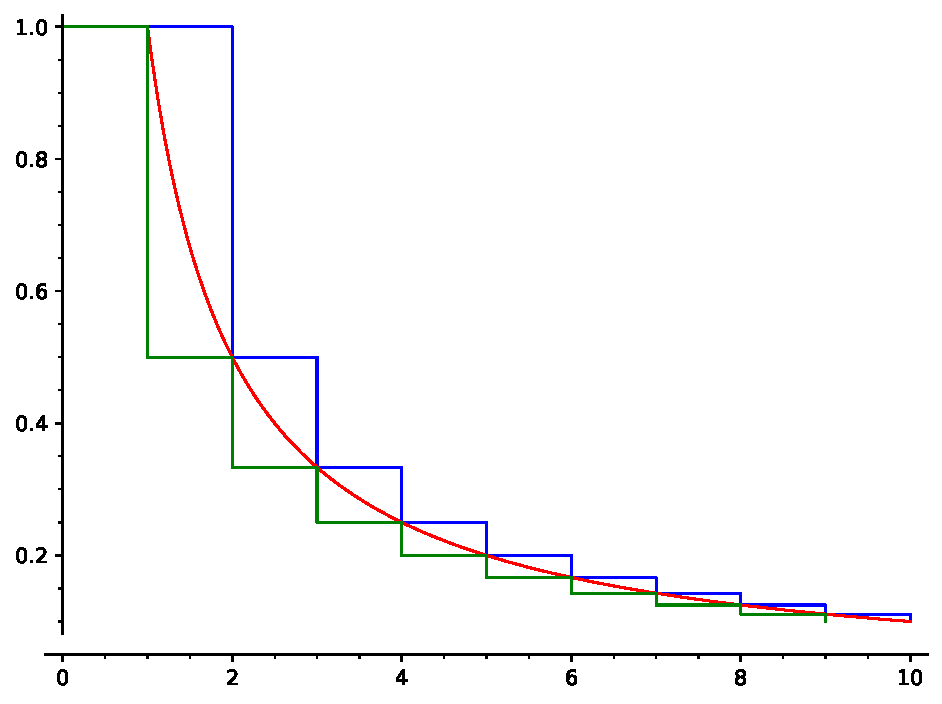
\includegraphics[height=50mm]{images/harmonic.pdf}
	\caption{Approximation der harmonischen Zahl durch den Logarithmus.}\label{fig_harmonic}
\end{figure}

Die Formel aus \Thm~\ref{thm_qs} ist recht genau, aber die Gr\"o\ss enordnung der Zahl der Vergleiche ist daraus nicht ganz leicht abzulesen.
Wir m\"ussen uns also mit dem asymptotischen Verhalten der harmonischen Zahl befassen.
Dazu erinnern wir uns an die Formel
\begin{align}\label{eqlog}
	\log x&=\int_1^x\frac1z\dd z&&(x>0).
\end{align}
Weil die Funktion $z\mapsto 1/z$ f\"ur $z>0$ monoton f\"allt, sehen wir (s.\ Abb.~\ref{fig_harmonic}), da\ss
\begin{align}\label{eqharm}
	\log n=\int_1^n\frac{\dd z}z\leq H_n&\leq1+\int_1^n\frac{\dd z}z=1+\log n.
\end{align}
Die Ungleichungen \eqref{eqharm} zeigen also, da\ss\ $H_n=O(1)+\log n$.
Aus \Thm~\ref{thm_qs} folgt also, da\ss\ Quicksort auf einer zuf\"alligen Permutation in Erwartung $O(n\log n)$ Vergleiche ausf\"uhrt.
Genauer zeigt der Beweis sogar, da\ss\ die erwartete Zahl der Vergleiche $(2+o(1))n\log n$ betr\"agt.
Die Folge der Differenzen
	\begin{align*}
		\lim_{n\to\infty}H_n-\log n
	\end{align*}
konvergiert \"ubrigens.
Der Grenzwert wird {\em Euler-Mascheroni-Konstante} genannt.

\subsection{Randomisiertes Quicksort}\label{sec_randomised_qs}
Die Analyse von Quicksort auf zuf\"alligen Permutationen f\"uhrt uns zu einer Modifikation des Algorithmus'.
Anstatt stets das erste Element als Pivot zu verwenden, zieht diese Modifikation ein zuf\"alliges Pivot-Element.

\begin{algorithm}\upshape {\tt RQuicksort}. {\em Eingabe:} eine Liste $L=(\ell_1,\ldots,\ell_n)$ vergleichbarer Elemente.\label{alg_rqs}
	{\em Ausgabe:} die Elemente in aufsteigender Reihenfolge.
	\begin{enumerate}
		\item Vertausche $\ell_1$ mit einem zuf\"alligen Element $\ell_i$, $i=1,\ldots,n$.
		\item F\"ur $i=1,\ldots,n$
		\item $\quad$falls $\ell_i<\ell_1$, f\"uge $\ell_i$ der Liste $K$ hinzu.
		\item $\quad$falls $\ell_i>\ell_1$, f\"uge $\ell_i$ der Liste $G$ hinzu.
		\item $\quad$falls $\ell_i=\ell_1$, f\"uge $\ell_i$ der Liste $M$ hinzu.
		\item Wende {\tt Quicksort} rekursiv an, um $K$ und $G$ zu sortieren.
		\item Gib $K,M,G$ aus.
	\end{enumerate}
\end{algorithm}

Bis auf den ersten Schritt ist also alles beim alten geblieben.
Ein Blick auf den Beweis von \Thm~\ref{thm_qs} zeigt, da\ss\ wir lediglich verwendet haben, da\ss\ das Pivotelement zuf\"allig ist.
Dies ist automatisch der Fall, wenn wir Algorithmus~\ref{alg_qs} auf eine zuf\"allige Permutationen anwenden, w\"ahrend Algorithmus~\ref{alg_rqs} die Zuf\"alligkeit des Pivots ausdr\"ucklich herstellt.
Dieselbe Analyse ist also auf beide Algorithmen anwendbar, so da\ss\ wir folgendes Ergebnis erhalten.

\begin{corollary}\label{cor_qs}
	F\"ur eine beliebige Liste $L$ ist die erwartete Zahl von Vergleichen, die RQuicksort durchf\"uhrt, von der Ordnung $O(n\log n)$.
\end{corollary}

Statt den Algorithmus auf einer zuf\"alligen Eingabe zu analysieren, haben wir also den Zufall in den Algorithmus selbst eingebaut.
Einen Algorithmus, der den Zufall als Hilfsmittel heranzieht, nennt man {\em randomisiert}.

Die wenigsten realen Computer verf\"ugen \"uber einen ``echten'' Zufallsgenerator, der gro\ss e Mengen von Zufallszahlen produzieren kann.
In der Praxis werden randomisierte Algorithmen daher in der Regel unter Verwendung eines Pseudozufallsgenerators implementiert.
Dabei sollte man sich der Begrenzungen eines solchen Pseudozufallsgenerators bewu\ss t sein.

\subsection{Die informationstheoretische Schranke}\label{sec_inf}
Au\ss er dem randomisierten Quicksort-Algorithmus gibt es verschiedene weitere (deterministische) Sortieralgorithmen, die f\"ur Listen beliebiger vergleichbarer Elemente eine Laufzeit (Zahl von Vergleichen) von $O(n\log n)$ erreichen.
Ein Beispiel, das Sie aus DAP1 kennen, ist Mergesort.
Jedoch gibt es keinen ``vergleichenden'' Algorithmus, der eine asymptotisch bessere Laufzeit, also $o(n\log n)$ Vergleiche, erzielt.
Es stellt sich heraus, da\ss\ das kein Zufall ist.
Denn es gibt eine informationstheoretische untere Schranke f\"ur vergleichsbasierte Algorithmen von $\Omega(n\log n)$.
In diesem Abschnitt leiten wir diese Schranke f\"ur deterministische Sortieralgorithmen her.
Sie gilt aber ebenso f\"ur randomisierte Algorithmen.

Genau gesagt ist ein {\em vergleichsbasierter Sortieralgorithmus} ein Sortieralgorithmus, der auf seine Eingabe nur durch Vergleichsanfragen $(\ell_i,\ell_j)$ zugreift.
Das Ergebnis einer solchen Vergleichsanfrage ist entweder ``kleiner'', ``gleich'' oder ``gr\"o\ss er''.
Wir repr\"asentieren diese drei Werte durch $-1,0,1$.
Aufgrund der Antworten auf diese Vergleichsanfragen entscheidet der Algorithmus dann \"uber die Reihenfolge der Elemente in der Ausgabe.
Wir analysieren solche Algorithmen jetzt bei Eingabe zuf\"alliger Permutationen und werden zeigen, da\ss\ die erwartete Zahl der Vergleichsanfragen mindestens von der Ordnung $\Omega(n\log n)$ ist.
Wir beginnen mit dem Beweis des folgenden Satzes.

\begin{theorem}\label{thm_inf}
	Angenommen $\cA$ ist ein deterministischer vergleichsbasierter Sortieralgorithmus.
	Sei $X_n(\cA)$ die erwartete Zahl von Vergleichen, die $\cA$ zum Sortieren einer zuf\"alligen $n$-Permutation $\vec\sigma$ durchf\"uhrt.
	Dann gilt $$X_n(\cA)=\Omega(\log(n!)).$$
\end{theorem}
\begin{proof}
	Sei $N(\sigma)$ die Zahl der Vergleiche, die der Algorithmus auf Eingabe $\sigma$ durchf\"uhrt.
	Wir wenden den Sortieralgorithmus an auf eine ``Tabelle'', deren erste Spalte aus der Permutation $\vec\sigma$ besteht und deren zweite Spalten einfach die geordneten Zahlen $1,\ldots,n$ enth\"alt:
	\begin{align*}
		\begin{array}{|c|c|}\hline\vec\sigma(1)&1\\\hline\vec\sigma(2)&2\\\hline\vdots&\vdots\\\hline\vec\sigma(n)&n\\\hline\end{array}
	\end{align*}
	Die Vergleichsoperation auf den Zeilen der Tabelle ist einfach dadurch definiert, da\ss\ die Zahlen in der ersten Spalte verglichen werden.
	Die zweite Spalte wird vom Algorithmus nur ``mitgef\"uhrt''.
	Die Ausgabe des Algorithmus' ist dann die sortierte Liste
	\begin{align}\label{eqthm_inf1}
		\begin{array}{|c|c|}\hline1&\vec\sigma^{-1}(1)\\\hline2&\vec\sigma^{-1}(2)\\\hline\vdots&\vdots\\\hline n&\vec\sigma^{-1}(n)\\\hline\end{array}
	\end{align}
	Die zweite Spalte der sortierten Tabelle enth\"alt also die inverse Permutation $\vec\sigma^{-1}$.
	Weil die Abbildung $\sigma\in\SS_n\mapsto\sigma^{-1}$ bijektiv ist, kann die Permutation $\vec\sigma$ aus der zweiten Spalte rekonstruiert werden.
(Dazu k\"onnten wir beispielsweise die beiden Spalten vertauschen und anschlie\ss end nochmal sortieren, denn $(\sigma^{-1})^{-1}=\sigma$.)
Beim Sortiervorgang geht also keine Information ``verloren''.

	Weil der Sortieralgorithmus deterministisch ist, sind seine Schritte vollst\"andig durch die Antworten auf die Vergleichsanfragen, die der Algorithmus stellt, bestimmt.
	Diese Antworten k\"onnen wir in einem Vektor $\va(\vec\sigma)=(a_1(\vec\sigma),\ldots,a_{N(\vec\sigma)}(\vec\sigma))\in\{0,\pm1\}^{N(\vec\sigma)}$ zusammenfassen.
	Weil bei dem Sortiervorgang keine Information verlorengeht (s.~\eqref{eqthm_inf1}), ist die Abbildung $\sigma\mapsto\va(\sigma)$ also eine Bijektion.

	Nehmen wir nun an, die erwartete Zahl $X_n(\cA)=\ex[N(\vec\sigma)]$ von Vergleichsanfragen, die der Algorithmus stellt, w\"are kleiner als $\eps n\log n$ f\"ur eine kleine Zahl $\eps>0$.
	Betrachte die Menge $S$ aller Permutationen $\sigma$, so da\ss\ $N(\vec\sigma)\leq\lceil 2\eps n\log n\rceil$.
	Dann erhalten wir%
	\footnote{Dieser Schritt ist auch als ``Markov-Ungleichung'' bekannt.}
	\begin{align*}
		\eps n\log(n)\geq X_n(\cA)&=\ex[N(\vec\sigma)]=\frac1{n!}\sum_{\sigma\in\SS_n}N(\sigma)\geq\frac1{n!}\sum_{\sigma\in\SS_n\setminus S}N(\sigma)\geq\frac{n!-|S|}{n!}\cdot2\eps n\log n,
	\end{align*}
	woraus wir schlie\ss en, da\ss\
	\begin{align}\label{eqthm_inf2}
		|S|\geq\frac{n!}2.
	\end{align}
	Ferner gibt es insgesamt nur 
	\begin{align*}
		\sum_{i=0}^h3^i\leq 3^{h+1}
	\end{align*}
	m\"ogliche Sequenzen $\va(\sigma)$ der L\"ange kleiner oder gleich $h$.
	Also schlie\ss en wir aus \eqref{eqthm_inf2}, da\ss
	\begin{align*}
		\frac{n!}2\leq|S|\leq 3^{h+1}.
	\end{align*}
	Umstellen nach $h$ liefert die Behauptung.
\end{proof}

\subsection{Die Stirling-Formel}\label{sec_stirling}
Wiederum ist es auf den ersten Blick nicht ganz offensichtlich, wie die Gr\"o\ss enordnung des Terms $\log(n!)$ aus \Thm~\ref{thm_inf} einzusch\"atzen ist.
Wir ben\"otigen dazu eine Absch\"atzung von $n!$.
Die Stirlingformel liefert diese Absch\"atzung.

\begin{theorem}\label{thm_stirling}
	Es gilt $n!\sim\sqrt{2\pi n}\bcfr n\eul^n$.
\end{theorem}

Zusammen mit \Thm~\ref{thm_inf} zeigt \Thm~\ref{thm_stirling}, da\ss\ vergleichsbasierte Sortieralgorithmen auf zuf\"alligen Permutation $\Omega(n\log n)$ Vergleiche ben\"otigen.
Quicksort ist also, zumindest was die Gr\"o\ss enordnung angeht, bestm\"oglich.

Wir fahren fort mit dem Beweis von \Thm~\ref{thm_stirling}, wobei wir~\cite{Lang} folgen.
Wir werden sogar die genauere Formel
\begin{align*}
	n!&=(1+O(1/n))\sqrt{2\pi n}\bcfr n\eul^n
\end{align*}
herleiten.
Dazu beginnen wir mit dem {\em Wallisschen Produkt}.

\begin{lemma}\label{lem_wallis}
	Es gilt
	\begin{align*}
		\frac{\pi}2&=\lim_{n\to\infty}\prod_{i=1}^n\frac{4i^2}{4i^2-1}.
	\end{align*}
\end{lemma}
\begin{proof}
	Partielle Integration zeigt, da\ss\ f\"ur $n\geq2$,
	\begin{align*}
		\int\sin^n(x)\dd x&=-\frac{\cos(x)\sin^{n-1}(x)}n+\frac{n-1}n\int\sin^{n-2}(x)\dd x.
	\end{align*}
	Weil $\sin(0)=\cos(\pi/2)=0$, folgt daraus mit Induktion nach $n$, da\ss
	\begin{align}\label{eqlem_wallis1}
		\int_0^{\pi/2}\sin^{2n}(x)\dd x&=\frac\pi2\prod_{i=1}^n\frac{2i-1}{2i},&
		\int_0^{\pi/2}\sin^{2n+1}(x)\dd x&=\prod_{i=1}^n\frac{2i}{2i+1}.
	\end{align}
	Ferner gilt f\"ur $n\geq1$, da\ss\
	\begin{align}\label{eqlem_wallis2}
		\frac{2n}{2n+1}\leq\frac{\int_0^{\pi/2}\sin^{2n+1}(x)\dd x}{\int_0^{\pi/2}\sin^{2n-1}(x)\dd x}\leq\frac{\int_0^{\pi/2}\sin^{2n+1}(x)\dd x}{\int_0^{\pi/2}\sin^{2n}(x)\dd x}\leq1;
	\end{align}
	erste Ungleichung folgt aus der rechten Formel aus \eqref{eqlem_wallis1}.
	Die zweite Ungleichung in \eqref{eqlem_wallis2} folgt daraus, da\ss\ $0\leq\sin^{2n}(x)\leq\sin^{2n-1}(x)$ f\"ur alle $x\in[0,\pi/2]$.
	Die dritte Ungleichung folgt analog aus $0\leq\sin^{2n+1}(x)\leq\sin^{2n}(x)$ f\"ur alle $x\in[0,\pi/2]$.
	Aus \eqref{eqlem_wallis2} folgt also, da\ss
	\begin{align}\label{eqlem_wallis3}
		\lim_{n\to\infty}\frac{\int_0^{\pi/2}\sin^{2n+1}(x)\dd x}{\int_0^{\pi/2}\sin^{2n}(x)\dd x}=1.
	\end{align}
	Indem wir nun \eqref{eqlem_wallis1} in \eqref{eqlem_wallis3} einsetzen, erhalten wir
	\begin{align*}
		\frac\pi2&=\lim_{n\to\infty}\prod_{i=1}^n\frac{(2i-1)(2i+1)}{(2i)^2}=\lim_{n\to\infty}\prod_{i=1}^n\frac{4i^2}{4i^2-1},
	\end{align*}
	wie behauptet.
\end{proof}

\begin{corollary}\label{cor_wallis}
Es gilt
\begin{align*}
	\frac{(n!)^22^{2n}}{(2n)!\sqrt n}\sim\sqrt\pi.
\end{align*}
\end{corollary}
\begin{proof}
	Wir schreiben das Wallissche Produkt als
	\begin{align*}
		\frac\pi2&\sim\prod_{i=1}^n\frac{(2i)^2}{(2i-1)(2i+1)}\sim\frac1{2n+1}\prod_{i=1}^n\frac{(2i)^2}{(2i-1)^2}\sim\frac1{2n}\prod_{i=1}^n\frac{(2i)^2}{(2i-1)^2};
	\end{align*}
	denn im Nenner des ersten Produkts tritt jede ungerade Zahl zweimal auf, mit Ausnahme von $2n+1$.
	Nun ziehen wir die Quadratwurzel:
	\begin{align}\label{eqcor_wallis1}
		\sqrt{\pi}&\sim\frac1{\sqrt{n}}\prod_{i=1}^n\frac{2i}{2i-1}.
	\end{align}
	Schlie\ss lich rechnen wir nach, da\ss\ $\prod_{i=1}^n\frac{2i}{2i-1}=\frac{(n!)^22^{2n}}{(2n)!}$.
	\begin{align}\label{eqcor_wallis2}
		\prod_{i=1}^n(2i)&=n!\cdot2^n,&\prod_{i=1}^n(2i-1)&=\frac{(2n)!}{n!\cdot2^n}.
	\end{align}
	Wir kombinieren \eqref{eqcor_wallis1} und \eqref{eqcor_wallis2} und erhalten
	\begin{align*}
		\frac{(n!)^22^{2n}}{(2n)!\sqrt n}&=\frac1{\sqrt{n}}\prod_{i=1}^n\frac{2i}{2i-1}\sim\sqrt\pi,
	\end{align*}
	wie behauptet.
\end{proof}

\begin{proof}[Beweis von \Thm~\ref{thm_stirling}]
	Wir betrachten die beiden Folgen
	\begin{align*}
		a_n&=\frac{n^{n+\frac12}}{n!}\exp(-n),&b_n&=a_n\exp\bcfr1{12n}=\frac{n^{n+\frac12}}{n!}\exp\bc{-n+\frac1{12n}}.
	\end{align*}
	Dann gilt
	\begin{align}\label{eqthm_stirling0}
		\lim_{n\to\infty}\frac{a_n}{b_n}&=\lim_{n\to\infty}\exp\bc{-\frac1{12n}}=1.
	\end{align}
	Ferner erhalten wir 
	\begin{align*}
		\log a_n&=-n+\frac12\log n+\sum_{i=1}^n\log\frac ni,&\log b_n&=\frac1{12n}-n+\frac12\log n+\sum_{i=1}^n\log\frac ni.
	\end{align*}
	Folglich gilt
	\begin{align}\label{eqthm_stirling7}
		\log\frac{a_{n+1}}{a_n}&=\bc{n+\frac12}\log\frac{n+1}n-1,&
		\log\frac{b_{n+1}}{b_n}&=\bc{n+\frac12}\log\frac{n+1}n-1-\frac1{12}\bc{\frac1n-\frac1{n+1}}.
	\end{align}

	Wir werden nun die beiden Ausdr\"ucke auf den rechten Seiten dieser Ungleichungen absch\"atzen.
	Dazu definieren wir die Funktionen
	\begin{align*}
		\varphi(x)&=\frac12\log\bcfr{1+x}{1-x}-x,&\psi(x)&=\varphi(x)-\frac{x^3}{3(1-x^2)}.
	\end{align*}
	Die Ableitungen dieser Funktionen, die wir mit Hilfe der Formel~\eqref{eqlog} berechnen, sind
	\begin{align}\label{eqthm_stirling1}
		\varphi'(x)&=\frac{x^2}{1-x^2}\geq0,&\psi'(x)&=-\frac{2x^4}{3(1-x^2)^2}\leq0.
	\end{align}
	Aus \eqref{eqthm_stirling1} und $\varphi(0)=0$ folgt $\varphi(x)\geq0$ f\"ur $0\leq x<1$.
	Entsprechend folgt aus $\psi(0)=0$, da\ss\ $\psi(x)\leq0$ f\"ur alle $0\leq x<1$.
	Daher erhalten wir die Ungleichungen
	\begin{align}\label{eqthm_stirling2}
		0\leq\frac12\log\bcfr{1+x}{1-x}-x&\leq\frac{x^3}{3(1-x^2)}&&(0\leq x<1).
	\end{align}
	Setze nun $x=1/(2n+1)$, so da\ss\
	\begin{align}\label{eqthm_stirling3}
		\frac{1+x}{1-x}&=\frac{n+1}n,&\frac{x^3}{3(1-x^2)}&=\frac1{12(2n+1)(n^2+n)}.
	\end{align}
	Zusammen mit \eqref{eqthm_stirling3} zeigt \eqref{eqthm_stirling2} dann
	\begin{align}%\label{eqthm_stirling4}
		0&\leq\frac12\log\bcfr{n+1}n-\frac1{2n+1}\leq\frac1{12(2n+1)(n^2+n)},\qquad\mbox{so da\ss}\nonumber\\
		0&\leq\bc{n+\frac12}\log\bcfr{n+1}n-1\leq\frac1{12}\bc{\frac1n-\frac1{n+1}}.\label{eqthm_stirling4}
	\end{align}

	In Kombination mit \eqref{eqthm_stirling7} zeigt \eqref{eqthm_stirling4} nun, da\ss\ $a_{n+1}\geq a_n$ und $b_{n+1}\leq b_n$ f\"ur alle $n$.
	Weil $a_1\leq b_1$, folgt aus \eqref{eqthm_stirling0} also, da\ss\ die Grenzwerte
	\begin{align}\label{eqthm_stirling6}
		c=\lim_{n\to\infty}a_n=\lim_{n\to\infty}b_n
	\end{align}
	existieren und \"ubereinstimmen, und da\ss\ $a_n\leq c\leq b_n$ f\"ur alle $n$.
	Umformen ergibt also, da\ss
	\begin{align}\label{eqthm_stirling5}
		n^{n+\frac12}\bcfr{n}\eul^n\leq c\cdot n!\leq\exp\bcfr1{12n}n^{n+\frac12}\bcfr{n}\eul^n.
	\end{align}

	Wir m\"ussen zuletzt noch $c$ berechnen.
	Dazu setzen wir in \eqref{eqthm_stirling6} gerade Werte von $n$ ein:
	\begin{align}\nonumber
	c&=\lim_{n\to\infty}a_{2n}=\lim_{n\to\infty}\frac{(2n)^{2n+\frac12}\exp(-2n)}{(2n)!}=\sqrt2\lim_{n\to\infty}\frac{(n!)^22^{2n}}{(2n)!\sqrt n}\bcfr{n^{n+\frac12}\exp(-n)}{n!}^2\\
	 &=\sqrt{2\pi}\lim_{n\to\infty}a_n^2=\sqrt{2\pi}c^2\qquad[\mbox{nach \Cor~\ref{cor_wallis}}].\label{eqthm_stirling8}
	\end{align}
	Weil $c>0$ folgt aus \eqref{eqthm_stirling8}, da\ss\ $c=1/\sqrt{2\pi}$.
	Einsetzen dieser Zahl in \eqref{eqthm_stirling5} beschlie\ss t den Beweis.
\end{proof}

\subsection{Binomialkoeffizienten}\label{sec_binom}
In der Analyse von Algorithmen begegnet oft der {\em Binomialkoeffizient}: f\"ur $0\leq k\leq n$ ist dieser definiert als
\begin{align*}
	\binom nk&=\frac{n!}{k!\cdot(n-k)!};
\end{align*}
Sprechweise: ``$n$ \"uber $k$''.
Falls $k>n\geq0$ definieren wir ferner $\binom nk=0$.

Aus der Schule wissen Sie vielleicht, da\ss\ Binomialkoeffizienten auf dem Weg \"uber das ``Pascalsche Dreieck'' berechnet werden k\"onnen.
Lassen Sie uns dies kurz herleiten.

\begin{lemma}\label{lem_pascal}
	F\"ur alle $0<k<n$ gilt
	\begin{align*}
		\binom nk&=\binom{n-1}{k-1}+\binom{n-1}k.
	\end{align*}
\end{lemma}
\begin{proof}
	Wir berechnen
	\begin{align*}
		\binom{n-1}{k-1}+\binom{n-1}k&=\frac{(n-1)!}{(k-1)!(n-k)!}+\frac{(n-1)!}{k!(n-k-1)!}=\frac{(n-1)!\cdot(k+(n-k))}{k!(n-k)!}=\binom nk,
	\end{align*}
	wie behauptet.
\end{proof}

Als unmittelbare Anwendung erhalten wir folgende kombinatorische Interpretation des Binomialkoeffizienten.

\begin{corollary}\label{cor_pascal}
	F\"ur $0\leq k\leq n$ z\"ahlt $\binom nk$ die $k$-elementigen Teilmengen von $[n]=\{1,\ldots,n\}$.
\end{corollary}
\begin{proof}
	Sei $T(n,k)$ die Zahl der $k$-elementigen Teilmengen von $[n]$.
	Dann gilt
	\begin{align*}
		T(n,k)&=T(n-1,k-1)+T(n-1,k).
	\end{align*}
	Denn eine $k$-elementige Teilmenge enth\"alt entweder das Element $n$, oder sie enth\"alt nicht das Element $n$.
	Die Zahl ersterer Teilmengen ist $T(n-1,k-1)$, die Zahl letzterer ist $T(n-1,k)$.
	Ferner gilt $T(n,0)=1$ f\"ur alle $n\geq1$ (leere Teilmenge).
	Weil $\binom n0=1$ f\"ur alle $n$, zeigt \Lem~\ref{lem_pascal}, da\ss\ $T(n,k)=\binom nk$ f\"ur alle $n,k$.
\end{proof}

\begin{corollary}[``binomischer Lehrsatz'']\label{cor_binom}
	F\"ur alle $a,b\in\RR$ und alle $n\in\NN$ gilt
	\begin{align*}
		(a+b)^n&=\sum_{k=0}^n\binom nka^kb^{n-k}.
	\end{align*}
\end{corollary}
\begin{proof}
	Wir f\"uhren Induktion nach $n$.
	F\"ur $n=1$ ist nichts zu zeigen.
	Ferner erhalten wir mittels \Lem~\ref{lem_pascal}
	\begin{align*}
		(a+b)^{n+1}&=(a+b)\cdot(a+b)^n=(a+b)\sum_{k=0}^n\binom nka^kb^{n-k}\\
				   &=\sum_{k=0}^n\binom{n}ka^{k+1}b^{n-k}+\sum_{k=0}^n\binom{n}ka^{k}b^{n-(k-1)}\\
				   &=a^{n+1}+\sum_{k=1}^n\binom{n}{k-1}a^kb^{n+1-k}+\sum_{k=1}^n\binom nka^kb^{n+1-k}+b^{n+1}\\
				   &=a^{n+1}+b^{n+1}+\sum_{k=1}^n\binom{n+1}ka^kb^{n+1-k}=\sum_{k=0}^{n+1}\binom {n+1}ka^kb^{n+1-k},
	\end{align*}
	was den Induktionsschritt zeigt.
\end{proof}

Eine direkte Konsequenz des binomischen Lehrsatzes ist die Aussage, da\ss\ die Menge $[n]$ insgesamt genau $2^n$ Teilmengen besitzt.
Denn
\begin{align*}
	2^n&=(1+1)^n=\sum_{k=0}\binom nk,
\end{align*}
und rechts steht nach \Cor~\ref{cor_pascal} die Zahl aller Teilmengen von $[n]$.

\section{Heapsort}\label{sec_heap}

Quicksort ist einfach und ``normalerweise'' schnell.
Aber die Laufzeit $O(n\log n)$ ist nicht {\em deterministisch} garantiert, sondern tritt nur mit hoher Wahrscheinlichkeit auf.
Au\ss erdem ben\"otigt der Algorithmus einen Zufallsgenerator.

Heapsort ist ein deterministischer Sortieralgorithmus, der die Vorteile von Quicksort teilt.
Im Gegensatz zu Mergesort ist Heapsort au\ss erdem speichereffizienter.
Heapsort ist ferner der erste Algorithmus, den wir kennenlernen, der als Kernelement eine clevere Datenstruktur benutzt.
Geeignete Datenstrukturen sind nicht selten ein wichtiges Hilfsmittel beim Algorithmenentwurf und k\"onnen zu wesentlichen Effizienzstigerungen f\"uhren.

Wir beginnen mit der Datenstruktur, die Heapsort verwendet.
Anschlie\ss end werden wir sehen, wie die Datenstruktur zum Sortieren verwendet wird.
Zum Schlu\ss\ sehen wir eine weitere Anwendung der Datenstruktur, n\"amlich ``priority queues''.

\subsection{Heaps}\label{sec_heaps}
Ein {\em Heap} ist eine Datenstruktur, die in einem Array abgespeichert werden kann.
Es ist hilfreich, sich diese Datenstruktur als einen Baum mit einer ausgezeichneten Wurzel vorzustellen.
In diesem Baum hat jeder Knoten h\"ochstens zwei Kinder.
Genauer gesagt entsteht der Baum aus einem vollst\"andigen Bin\"arbaum, in dem jeder Knoten in Blatt ist oder genau zwei Kinder hat, indem ggf.\ einige der Bl\"atter gel\"oscht werden.

Um dies zu pr\"azisieren, werden wir zu einem Array $\vA=(A_1,\ldots,A_n)$ mit $n$ Elementen einen gewurzelten Baum $B(\vA)$ konstruieren.
Der Baum hat Knoten $v_1,\ldots,v_n$.
Die Wurzel des Baumes ist ein Knoten $v_1$.
Das linke Kind eines Knoten $v_i$ ist der Knoten $v_{2i}$, falls $2i\leq n$.
Wenn $2i>n$, hat der Knoten $v_i$ keine Kinder.
Das rechte Kind von Knoten $v_i$ ist der Knoten $v_{2i+1}$, falls $2i+1\leq n$.
Andernfalls hat $v_i$ kein rechtes Kind.
Der Elternknoten eines Knoten $v_i$, $i\geq2$, ist der Knoten $v_{\lfloor i/2\rfloor}$.
Im Knoten $v_i$ wird das $i$-te Element $A_i$ des Arrays gespeichert.
Mit Hilfe dieses Schemas k\"onnen wir also die Knoten des Baumes bijektiv auf die Arrayeintr\"age abbilden.

Wir nehmen an, da\ss\ die Elemente $A_i$ des Arrays vergleichbar sind.
F\"ur je zwei Elemente $A_i,A_j$ gilt also entweder $A_i<A_j$, $A_i=A_j$ oder $A_i>A_j$.
Wie genau diese Relation definiert ist (z.B.\ ob es sich um Zahlen handelt oder Zeichenketten), ist nicht von Belang.

Wir nehmen weiterhin an, da\ss\ das Array $\vA$ einen Gr\"o\ss enparameter $\size(\vA)=n$ hat.
Dieser zeigt die Anzahl der Elemente des Heaps an.
(M\"oglicherweise ist f\"ur $\vA$ jedoch mehr Speicherplatz reserviert.)

Die wesentliche Eigenschaft der Datenstruktur ist, da\ss\ die Elemente $A_i$ entsprechend der Eltern-Kind-Struktur des Baumes angeordnet sind.
Es gibt zwei Varianten.
In einem {\em max-heap} werden die Elemente so angeordnet, da\ss\ das Element $A_i$, das im Elternknoten $v_i$ gespeichert ist, niemals kleiner ist als das Element $A_j$ in einem Kindknoten $v_j$.
In einem {\em min-heap} ist das Element im Elternknoten niemald gr\"o\ss er.
Wir werden uns hier ausschlie\ss lich mit max-heaps befassen.

Es stellt sich nat\"urlich die Frage, wie wir die zu sortierenden Eingabedaten in eine Heap-Struktur bringen.
Au\ss erdem erfordert der Sortiervorgang verschiedene Operationen auf der Datenstruktur.
Wir befassen uns daher mit zwei Hilfsoperationen: {\tt MaxHeapify} und {\tt BuildMaxHeap}.

\subsection{Die {\tt MaxHeapify}-Operation}\label{sec_maxheapify}
{\tt MaxHeapify} ist eine Hilfsfunktion, die wir zum Aufbau eines Heaps ben\"otigen.
Die Eingabe besteht aus einem Array $\vA$ und einem Index $i$.
Wir nehmen an, da\ss\ das Array so beschaffen ist, da\ss\ die Unterb\"aume ``unter'' den Kindern von $i$ bereits die max-heap-Eigenschaft haben.
Allerdings ist m\"oglicherweise das Element $A_i$ kleiner als eines seiner Kinderelemente.
Die Idee ist nun, das Element $A_i$ ``absinken'' zu lassen, bis die max-heap-Eigenschaft f\"ur den Unterbaum ``unter'' $i$ selbst erf\"ullt ist.

\begin{algorithm}\upshape {\tt MaxHeapify}$(\vA,i)$.\label{alg_maxheapify}
	\begin{enumerate}
		\item Wenn $A_i$ gr\"o\ss er ist als die Werte seiner Kinder oder $A_i$ kein Kind hat, halte. 
		\item Sonst bestimme gr\"o\ss te Kind $A_j$.
		\item Vertausche die Wert von $A_i$ und $A_j$.
		\item Rufe {\tt MaxHeapify}$(\vA,j)$ auf.
	\end{enumerate}
\end{algorithm}

Mit ``Laufzeit'' ist weiterhin die Zahl der durchgef\"uhren Vergleiche gemeint.
Die {\em H\"ohe} eines Knotens $i$ in $\vA$ ist der maximale direkte Abstand von $i$ von einem Blatt in dem Baum $B(\vA)$.
Wir beginnen mit folgender Beobachtung.

\begin{lemma}\label{lemma_highheap}
	Die H\"ohe der Wurzel in $B(\vA)$ ist $O(\log n)$.
\end{lemma}
\begin{proof}
	Indem wir den Baum ``auff\"ullen'', d\"urfen wir annehmen, da\ss\ $B(\vA)$ ein vollst\"andiger Bin\"arbaum ist.
	In diesem Fall sind die Pfade von der Wurzel zu allen Bl\"attern gleichlang.
	Ferner erf\"ullt die Zahl $N(h)$ der Knoten in einem solchen Baum der H\"ohe $h$ die Rekurrenz
	\begin{align*}
		N(h+1)&=1+2N(h),&N(0)&=1,
	\end{align*}
	weil die beiden Teilb\"aume ``unter'' den Kindern der Wurzel symmetrisch sind.
	
	Wir behaupten nun, da\ss\
	\begin{align}\label{eqlemma_highheap}
		N(h)=2^{h+1}-1.
	\end{align}
	Den Beweis f\"uhren wir per Induktion nach $h$.
	F\"ur $h=0$ ist die Behauptung offensichtlich.
	F\"ur den Induktionsschritt erhalten wir
	\begin{align*}
		N(h+1)&=1+2N(h)=1+2\cdot(2^{h+1}-1)=2^{h+2}-1,
	\end{align*}
	wie behauptet.
	Umstellen des Ausdrucks nach $h$ vervollst\"andigt den Beweis.
\end{proof}

\begin{proposition}\label{prop_maxheapify}
	Angenommen der Knoten $i$ has H\"ohe $h$.
	Die Laufzeit von {\tt MaxHeapify} betr\"agt $O(h)$.
\end{proposition}
\begin{proof}
	Sei $h$ die H\"ohe des Knotens $i$.
	Weil jeder Nachkomme von Knoten $i$ nur mit seinen direkten Kindern verglichen wird, ist die Zahl der Vergleichen wird, ist die Laufzeit $O(h)$.
\end{proof}

Als direkte Konsequenz aus \Lem~\ref{lemma_highheap} und \Prop~\ref{prop_maxheapify} erhalten wir folgendes.

\begin{corollary}\label{cor_maxheapify}
	{\tt MaxHeapify} hat Laufzeit $O(\log n)$. 
\end{corollary}

\subsection{Die {\tt BuildMaxHeap}-Operation}\label{sec_buildmaxheap}
Zweck von {\tt BuildMaxHeap} ist, aus einem beliebigen Array $\vA$ einen max-heap zu machen.
Dazu arbeiten wir uns von hinten nach vorn durch die Arrayeintr\"age und bauen den gew\"unschten Heap von unten nach oben auf.
Fur die zweite H\"alfte des Arrays ist zun\"achst nichts zu tun.
Diese Arrayeintr\"age bilden schlie\ss lich die Bl\"atter des Heaps und haben somit am Ende H\"ohe Null.
Auf die erste H\"alfte der Eintr\"age wenden wir nach und nach die {\tt MaxHeapify}-Operation an.

\begin{algorithm}\upshape {\tt BuildMaxHeap}$(\vA)$.\label{alg_buildmaxheap}
	\begin{enumerate}
		\item F\"ur $i=\lfloor n/2\rfloor,\ldots,1$
		\item $\quad${\tt MaxHeapify}$(\vA,i)$
	\end{enumerate}
\end{algorithm}

Die Analyse von {\tt MaxHeapify} stellt sicher, da\ss\ das Ergebnis von {\tt BuildMaxHeap} tats\"achlich ein max-heap ist.

\begin{proposition}\label{prop_buildmaxheap}
	{\tt BuildMaxHeap} hat Laufzeit $O(n)$.
\end{proposition}
\begin{proof}
	Wir wenden {\tt MaxHeapify} nacheinander auf alle Knoten an.
	Die H\"ohe $H$ der Wurzel ist nach \eqref{eqlemma_highheap} beschr\"ankt durch $\log_2n$.
	Die Zahl der Knoten mit Abstand $t$ von der Wurzel betr\"agt nach \eqref{eqlemma_highheap} h\"ochstens $2^{t+1}-1$.
	Nach \Prop~\ref{prop_maxheapify} ist die Laufzeit f\"ur eine {\tt MaxHeapify}-Operation beschr\"ankt durch $O(H-t)$.
	Weil die Funktion $x\mapsto x2^{-x}$ f\"ur $x\geq1/\log2$ monoton f\"allt, berechnet die Gesamtlaufzeit sich also zu
	\begin{align*}
		\sum_{t=1}^{H}(H-t)2^{t+1}\leq O(2^{H})\int_0^{\infty}x2^{-x}\dd x=
		-\frac{x\log(2)+1}{2^x\log(2)^2}\bigg|_0^\infty\cdot O(2^H)=O(2^H)=O(n),
	\end{align*}
	wie behauptet.
\end{proof}

\subsection{Der Heapsort-Algorithmus}\label{sec_hs}
Mit Hilfe der max-heap Datenstruktur ist es einfach, einen effizienten Sortieralgorithmus zu realisieren.
Die Eingabe des Algorithmus' ist ein Array $\vA$.

\begin{algorithm}\upshape {\tt Heapsort}$(\vA)$.\label{alg_heapsort}
	\begin{enumerate}
		\item {\tt BuildMaxHeap}$(\vA)$
		\item F\"ur $i=n,n-1,\ldots,2$
		\item $\quad$vertausche $A_1$ und $A_i$
		\item $\quad$wende {\tt MaxHeapify} an auf das Array $(A_1,\ldots,A_{i-1})$ und Element $1$ an
		\item gib $(A_1,\ldots,A_n)$ aus
	\end{enumerate}
\end{algorithm}

Der Algorithmus nutzt die Tatsache aus, da\ss\ $A_1$ stets das gr\"o\ss te Element des max-heaps ist.
Dieses wird stets genau mit dem letzten Element des max-heaps vertauscht und somit an die ``richtige'' Stelle verschoben.
Anschlie\ss end wird der max-heap um ein Element verk\"urzt.
Weil die Wurzel jetzt nicht mehr notwendigerweise das gr\"o\ss te Element ist (denn wir haben ja gerade das $i$-te Element an die erste Stelle getauscht), wird {\tt MaxHeapify} ausgef\"uhrt, um die max-heap Eigenschaft wiederherzustellen.

\begin{theorem}\label{thm_heapsort}
	{\tt Heapsort} sortiert ein gegebenes Array in Zeit $O(n\log n)$.
\end{theorem}
\begin{proof}
	Die Laufzeit f\"ur {\tt BuildMaxHeap} ist $O(n)$ nach \Prop~\ref{prop_buildmaxheap}.
	Ferner zeigt \Prop~\ref{prop_maxheapify}, da\ss\ jeder Aufruf von {\tt MaxHeapify} Zeit $O(\log n)$ beansprucht.
	Wir kommen somit auf eine Gesamtlaufzeit von $O(n\log n)$.
\end{proof}

\subsection{Priority queues}\label{sec_priority}
Die Datenstruktur max-heap hat weitere Anwendungen.
Dazu versehen wir die Datenstruktur mit einigen weiteren Funktionen.
Das resultierende Konstrukt wird als {\em priority queue} bezeichnet.
Entsprechend gibt es auch min-priority queues, die beispielsweise f\"ur die Berechnung k\"urzester Pfade verwendet werden k\"onnen.

In einer (max-)priority queue $\vA=(A_1,\ldots,A_n)$ ist es nat\"urlich leicht, das maximale Element zu finden: es ist einfach das Element $A_1$.
Eine weitere wichtige Operation ist die {\em Extraktion} des Maximums.
Hierbei wird das maximale Element aus der Datenstruktur entfernt.

\begin{algorithm}\upshape {\tt ExtractMax}$(\vA)$.\label{alg_extractmax}
	\begin{enumerate}
		\item falls $n=0$, abbrechen; falls $n=1$, gib $A_1$ aus und halte.
		\item vertausche $A_1$ und $A_n$
		\item wende {\tt MaxHeapify}$((A_1,\ldots,A_{n-1}),1)$ an
		\item gib $A_n$ und $(A_1,\ldots,A_{n-1})$ aus
	\end{enumerate}
\end{algorithm}

Die Vorgehensweise ist also \"ahnlich wie bei {\tt Heapsort}.
Wir vertauschen das letzte und das erste Element und bringen dann die Datenstruktur $(A_1,\ldots,A_{n-1})$ der L\"ange $n-1$ ``in Ordnung''.

Eine weitere Operation einer max-priority queue ist {\tt IncreaseKey}.
Diese Operation erh\"oht den Wert eines Elements auf einen gegebenen Wert $\alpha$.

\begin{algorithm}\upshape {\tt IncreaseKey}$(\vA,i,\alpha)$.\label{alg_increasekey}
	\begin{enumerate}
		\item falls $\alpha<A_i$, brich ab
		\item setzte $A_i=\alpha$
		\item solange $i>1$
		\item $\quad$setze $j=\lfloor i/2\rfloor$ \hfill\# $j=$Elternknoten von $A_i$
		\item $\quad$falls $A_j\geq\alpha$, halte
		\item $\quad$falls $A_j<\alpha$, vertausche $A_j$ und $\alpha$
		\item $\quad$setze $i=j$
	\end{enumerate}
\end{algorithm}

Der $i$-te Knoten steigt also in der Datenstruktur auf, bis die max-heap-Eigenschaft wiederhergestellt ist.

Schlie\ss lich ben\"otigen wir eine Operation, die neue Elemente in die Datenstruktur einf\"ugt.
Dazu f\"uge wir ein neues Element mit einem k\"unstlichen Wert $-\infty$, der als kleiner gilt als alle anderen Werte, in die Datenstruktur ein.
Anschlie\ss end wenden wir {\tt IncreaseKey} an.

\begin{algorithm}\upshape {\tt Insert}$(\vA,i,\alpha)$.\label{alg_insert}
	\begin{enumerate}
		\item f\"uge ein Element $\vA_{n+1}=-\infty$ zu $\vA$ hinzu
		\item wende {\tt IncreaseKey}$((A_1,\ldots,A_{n+1},n+1,\alpha)$ an
	\end{enumerate}
\end{algorithm}

Wenn wir annehmen, da\ss\ der Speicherplatz $A_{n+1}$ verf\"ugbar ist, dann l\"a\ss t sich der erste Schritt des Algorithmus' effizient implementieren.
Andernfalls mu\ss\ das Array ggf.\ umkopiert werden.
F\"ur die folgende Aussage verwenden wir ``Laufzeit'' wiederum gleichbedeutend mit ``Vergleichen''.

\begin{proposition}\label{prop_priority}
	Die Operationen {\tt ExtractMax}, {\tt IncreaseKey} und {\tt Insert} haben Laufzeit $O(\log n)$.
\end{proposition}
\begin{proof}
	Dies folgt unmittelbar aus \Lem~\ref{lemma_highheap}.
\end{proof}

\begin{remark}\label{rem_min}\upshape
	\Prop~\ref{prop_priority} l\"a\ss t sich entsprechend auf min-priority-queues \"ubertragen.
	In diesem Fall stehen die Operationen {\tt ExtractMin} und {\tt DecreaseKey} zur Verf\"ugung.
	Werden als Schl\"ussel Zahlen verwendet, besteht die einfachste Umsetzung darin, eine max-priority-queue auf die {\em negierten} Schl\"usselwerte anzuwenden.
\end{remark}

\section{Die Registermaschine}\label{sec_ram}
In diesem Abschnitt, der~\cite{Papadimitriou} folgt, befassen wir uns mit der Registermaschine (``random access machine'').
Diese erm\"oglicht eine exakte Definition von ``Laufzeit''.
Wir werden die Registermaschine nur (relativ) informell einf\"uhren.
Eine vollst\"andige formale Abhandlung ist in~\cite{Papadimitriou} zu finden.

\subsection{Definition}\label{sec_ram_def}
Es gibt verschiedene formale (d.h.\ mathematische) Modelle von realen Computern oder Computerprogrammen.
Ein bekanntes Modell, von dem Sie wom\"oglich schon geh\"ort haben, ist die Turingmaschine.
Allerdings ist die ``Hardware'' der Turingmaschine (im wesentlichen ein unendlich langes Speicherband) modernen Computern sehr un\"ahnlich.
Aus diesem Grund ist sie ungeeignet, um reale Laufzeit realistisch abzubilden.

Die {\em Registermaschine} ist besser geeignet.
Ihre ``Hardware'' besteht aus einer unendlichen Zahl von {\em Registern} $(r_i)_{i\geq0}$, von denen jedes eine ganze Zahl speichern kann.
Die Register \"ahneln also den RAM-Speicherzellen eines realen Computers, bis auf die Tatsache, da\ss\ die Wortgr\"o\ss e unbeschr\"ankt ist.
Das Register $r_0$ spielt eine besondere Rolle, n\"amlich die des ``Akkumulators''.
Das bedeutet, da\ss\ mit dem Wert dieses Registers Rechenoperationen durchgef\"uhrt werden k\"onnen.

Wie ein realer Computer auch, kann die Registermaschine programmiert werden.
Das Programm ist nicht ver\"anderbar, also sozusagen ``hart verdrahtet''.
Ein Registermaschinenprogramm besteht aus einer geordneten Abfolge von Befehlen, die in aufsteigend numerierten Zeilen daherkommen.
Die Registermaschine verf\"ugt \"uber einen Programmz\"ahler $z$, der die Zeilennummer der als n\"achstes auszuf\"uhrende Anweisung enth\"alt.
Anfangs hat der Z\"ahler den Wert $z=1$.

Das Programm der Registermaschine besteht aus folgenden Befehlen, wobei $j\in\NN_0$ und $x\in\ZZ$:

\begin{center}
\begin{tabular}{|l|l|}\hline
	{\tt read} $j$&schreibe den Wert von $r_j$ in $r_0$\\
	{\tt read} $*j$&wenn $h$ der Wert von $r_j$ ist, schreibe den Wert von $r_h$ in $r_0$\\
	{\tt store} $j$&schreibe den Wert von $r_0$ in $r_j$\\
	{\tt store} $*j$&wenn $h$ der Wert von $r_j$ ist, schreibe den Wert von $r_0$ in $r_h$\\
	{\tt load} $x$&schreibe die Zahl $x$ in $r_0$\\
	{\tt add} $x$&addiere $x$ zu der Zahl in $r_0$\\
	{\tt half}&wenn $y$ der Wert von $r_0$ ist, setze $r_0$ auf $\lfloor y/2\rfloor$\\
	{\tt jump} $j$&setze den Programmz\"ahler auf den Wert $j$\\
	{\tt jpos} $j$&wenn der Wert in $r_0$ positiv ist, f\"uhre {\tt jump} $j$ aus\\
	{\tt jneg} $j$&wenn der Wert in $r_0$ negativ ist, f\"uhre {\tt jump} $j$ aus\\
	{\tt jzero} $j$&wenn der Wert in $r_0$ gleich Null ist, f\"uhre {\tt jump} $j$ aus\\
	{\tt halt}&beende das Programm\\\hline
\end{tabular}
\end{center}

Bei Programmstart steht die Eingabe in Register $r_0$ und alle anderen Register haben den Wert $0$.
Entsprechend ist das Ergebnis der Berechnung ist der Inhalt von $r_0$.
Insbesondere sind also Eingabe und Ergebnis immer ganze Zahlen.
Die Semantik h\"angt von dem Programm ab.

Das Programm kann also verschiedene Codierungen der Eingabe vorsehen.
Beispielsweise kann eine Zeichenfolge mit dem ASCII-Code (oder einem anderen Code wie UTF8) in eine Zahl \"uberf\"uhrt werden.
Die Zeichenkette ``Hallo!'' w\"urde beispielsweise den ASCII-Codes 72, 97, 108, 108, 111, 33 entsprechen.
Im Hezadezimalsystem lauten diese Werte 48, 61, 6c, 6c, 6f, 21.
Um daraus die Eingabe zu codieren, bilden wir die Hexadezimalzahl 48616c6c6f21.
Der Dezimalwert dieser Zahl lautet
\begin{align*}
72\cdot256^5+97\cdot254^4+108\cdot256^3+108\cdot256^2+111\cdot256+33=79583268073249.
\end{align*}
Da wir prinzipiell jedes diskrete Objekt (Br\"uche, algebraische Ausdr\"ucke, Graphen, Grammatiken, logische Formeln, Matrizen, \ldots) als Zeichenketten darstellen k\"onnen, ist es m\"oglich, all diese Objekte mit einer Registermaschine zu verarbeiten.
Die Idee der Eingabecodierung als Zahlen ist offenbar der Codierung in einem realen Computer sehr \"ahnlich. 
Analog kann die Ausgabe interpretiert werden.
Beispielsweise kann ein Wert von $0$ oder $1$ ``Erfolg'' oder ``Mi\ss erfolg'' anzeigen.

Die Registermaschine hat ``nativ'' keine Operationen zur Addition, Multiplikation oder Division von Zahlen.
Jedoch k\"onnen diese Operationen mit den obigen Befehlen realisiert werden.
Dazu programmieren Sie im wesentlichen die Algorithmen, die Sie in der Grundschule kennengelernt haben.

Die M\"achtigkeit der Registermaschine w\"urde sich nicht wesentlich ver\"andern, wenn wir einen Befehl hinzuf\"ugen w\"urden, der den Inhalt eines gegebenen Registers zum Wert des Registers $r_0$ addiert.
Ein Multiplikationsbefehl hingegen w\"urde die Maschine wirklich m\"achtiger machen.
Denn wenn wir den Wert $2$ in Register $r_0$ einspeichern und dann $r_0$ mit sich selbst multiplizieren, so erhielten wir innerhalb von $n$ Operationen den Wert $2^{2^n}$.
Eine Registermaschine ohne Multiplikationsbefehl br\"auchte hingegen etwa $2^n$ Operationen, um denselben Wert zu erreichen.

\subsection{Effiziente Algorithmen}\label{sec_P}
Formal gesehen ist f\"ur uns ein Algorithmus also eine Registermaschine (ausgestattet mit einem Programm).
Die Registermaschine gibt uns daher ein Hilfsmittel zur Messung der Laufzeit eines Algorithmus' an die Hand.
Wir definieren also die Laufzeit $T_{\cM}(e)$ einer Registermaschine $\cM$ auf einer Eingabe $e\in\ZZ$ als die Zahl der Befehle, die die Maschine ausf\"uhrt bevor sie h\"alt.
Folglich gilt $T_\cM(e)\in\NN\cup\cbc\infty$.
Der Wert $\infty$ wird angenommen, wenn die Maschine gar nicht h\"alt.

Um den Begriff des {\em effizienten} Algorithmus zu definieren, fragen wir nach der Laufzeit von $\cM$ auf einer {\em gro\ss en} Eingabe.
Dazu definieren wir die {\em Eingabel\"ange} einer Zahl $e\in\ZZ$ als $\lceil\log_2(2+|e|)\rceil$.
Die Eingabel\"ange ist also die Anzahl Bits, die ben\"otigt werden, um $e$ in Bin\"ardarstellung zu schreiben.
Diese Begriffsbildung passt gut mit unserer obigen Codierung von Zeichenketten in Zahlendarstellungen zusammen.
Die Anzahl von Zeichen in einem festen Alphabet, die zur Eingabe einer Zeichenkette ben\"otigt werden, stimmt n\"amlich bis auf einen konstanten Faktor, also bis auf $\Theta(1)$, mit der Bitl\"ange \"uberein.

Wir nennen nun einen Algorithmus $\cM$ {\em effizient}, falls es eine Zahl $\ell\geq0$ gibt, so da\ss\ f\"ur die Funktion
\begin{align*}
	\cT_{\cM}(n)&=\max\cbc{T_\cM(e):\log_2(2+|e|)\leq n}
\end{align*}
gilt $\cT_{\cM}(n)=O(n^\ell)$.
Die Laufzeit von $\cM$ auf einer Eingabe der L\"ange $n$ skaliert also h\"ochstens als ein Polynom $n^\ell$ f\"ur $n\to\infty$.

\begin{definition}\label{def_P}
	Eine Funktion $f:\ZZ\to\ZZ$ hei\ss t {\em effizient berechenbar}, wenn es einen effizienten Algorithmus $\cM$ gibt, der f\"ur alle $e\in\ZZ$ bei Eingabe $e$ den Wert $f(e)$ ausgibt.
	Mit P wird ferner die Menge aller effizient berechenbaren Funktionen $f:\ZZ\to\{0,1\}$ bezeichnet.
\end{definition}

Interpretieren wir die Werte $0$ und $1$ als ``ja'' und ``nein'', so k\"onnen wir uns Funktionen $f:\ZZ\to\{0,1\}$ als Entscheidungsprobleme vorstellen.

Obiger Begriff der effizienten Berechenbarkeit ist nicht perfekt, hat sich aber in der Praxis bew\"ahrt.
Allerdings sind f\"ur viele wichtige Funktionen keine effizienten Algorithmen bekannt.
Stattdessen kennen wir h\"aufig nur Algorithmen, deren Laufzeit exponentiell in der Gr\"o\ss e der Eingabe skaliert. 
Diese Algorithmen sind in der Regel schon f\"ur moderat gro\ss e Eingaben nicht praktikabel.

Kommen wir zum Abschlu\ss\ noch einmal auf die Turingmaschine zur\"uck.
Die konkreten Laufzeitdefinition, wenn wir statt der Befehle einer Registermaschine die Schritte einer Turingmaschine z\"ahlen, \"andert sich ganz erheblich.
Was sich aber interessanterweise nicht \"andert, ist der Begriff der effizienten Berechenbarkeit.
Dieser ist gewisserma\ss en ``universell''.

In der GTI-Veranstaltung wird das Thema Laufzeiten weiter vertieft.
Dort wird auch die Klasse NP eingef\"uhrt, die die Klasse P enth\"alt.
Zus\"atzlich enth\"alt die Klasse NP viele Entscheidungsprobleme, f\"ur die wir bisher keine effizienten Algorithmen kennen.
Ob es solche Algorithmen gibt, ist die Essenz des br\"uhmten P$\neq$NP-Problems.

\section{Sortieren in linearer Zeit}\label{sec_radix}

\noindent
In Abschnitt~\ref{sec_inf} haben wir die informationstheoretische untere Schranke $\Omega(n\log n)$ f\"ur vergleichsbasierte Sortieralgorithmen kennengelernt.
In diesem Abschnitt lernen wir Sortieralgorithmen kennen, die eine lineare Laufzeit haben, sofern die Eingabedaten geeignet ``strukturiert'' sind.
Diese Algorithmen k\"onnen folglich nicht vergleichsbasiert sein.
Der Abschnitt folgt~\cite{Cormen}.

\subsection{Sortieren via Z\"ahlen}\label{sec_counting}
Wir nehmen an, da\ss\ die Elemente des zu sortierenden Arrays $\vA=(A_1,\ldots,A_n)$ jeweils mit einem \emph{Schl\"ussel} aus einer Menge $\cS=\{s_1,\ldots,s_k\}$ versehen sind.
Die Aufgabenstellung ist, die Elemente so zu sortieren, da\ss\ zuerste alle Elemente mit Schl\"ussel $s_1$, dann alle mit Schl\"uss el $s_2$ kommen, etc.
Dabei sollen Elemente $A_i$ mit {\em demselben} Schl\"ussel in derselben Reihenfolge ausgegeben werden, in der sie eingegeben wurden.
Man spricht in diesem Fall von einem \emph{stabilen} Sortieralgorithmus.

Der folgende Algorithmus l\"ost diese Aufgabe.

\begin{algorithm}{\tt CountingSort$(\vA,\cS)$}
	\begin{enumerate}
		\item Lege ein Hilfsarray $\vC=(C_1,\ldots,C_k)$ an, so da\ss\ $C_i$ die Zahl der Vorkommnisse von $s_i$ in $\vA$ enth\"ahlt.
		\item Verwende das Hilfsarray, um die Zahlen $C_i'$ der Elemente mit Schl\"usseln $s_1,\ldots,s_i$ zu bestimmen.
		\item Reserviere Speicherplatz $\vB=(B_1,\ldots,B_n)$ f\"ur das Ausgabearray
		\item F\"ur $j=n,\ldots,1$
		\item $\quad$ermittle den Schl\"ussel $\sigma$ von $A_j$
		\item $\quad$setze $B_{C'_\sigma}=A_j$
		\item $\quad$verringere $C'_\sigma$ um 1
	\end{enumerate}
\end{algorithm}

Die Stabilit\"at des Sortierverfahrens wird dadurch sichergestellt, da\ss\ wir in Schritt (4) die Elemente des Arrays von hinten nach vorn durchgehen.
Die Laufzeit des Verfahrens ist offenbar $O(n+k)$.

\subsection{Radixsort}\label{sec_radixsort}
Beim Radixsort-Verfahren nehmen wir an, da\ss\ die Elemente der Eingabeliste $\vA$ jeweils mit einer Folge von $d$ Schl\"usseln aus der Menge versehen sind.
Diese Folgen sind lexikographisch angeordnet.
Gewisserma\ss en ist also die Menge der Schl\"ussel nun $\cS^d$ mit der lexikographischen Ordnung.
Nat\"urlich k\"onnten wir das Array $\vA$ mit {\tt CountingSort} in Zeit $O(n+k^d)$ sortieren.
Es gibt aber eine bessere L\"osung: Radixsort.

\begin{algorithm}{\tt Radixsort$(\vA,\cS,d)$}
	\begin{enumerate}
		\item f\"ur $i=d,\ldots,1$
		\item $\quad$sortiere $\vA$ nach der $i$-ten Komponente des Schl\"ussels mit {\tt CountingSort}
	\end{enumerate}
\end{algorithm}

Wir verwenden also {\tt CountingSort} $d$ Mal mit der Schl\"usselmenge $\cS$, anstatt einmal mit $\cS^d$.
Wichtig ist, da\ss\ wir mit der $d$-ten, also der {\em geringwertigsten} Stelle des Gesamtschl\"ussels beginnen!
Unsere Analyse von {\tt CountingSort} liefert unmittelbar folgendes Ergebnis.

\begin{proposition}\label{prop_radix}
	{\tt Radixsort} hat Laufzeit $O(dn+dk)$.
\end{proposition}

Anstatt einer Laufzeit von $O(n+k^d)$ bekommen wir also lediglich eine Laufzeit $O(n+dk)$ heraus.
Schon f\"ur moderate Werte von $d,k$ ist das eine deutliche Verbesserung.
{\tt Radixsort} ist hervorragend geeignet, um nach alphanumerischen Schl\"usseln fester L\"ange oder nach Daten (``Tag--Monat--Jahr'') zu sortieren.

\section{Mediane und das Auswahlproblem}\label{sec_select}

\noindent
Gegeben ein Array $\vA=(A_1,\ldots,A_n)$ vergleichbarer Elemente, ist unser Ziel, das $\ell$-te Element (in aufsteigender Reihenfolge) auszuw\"ahlen.
Dazu k\"onnten wir selbstverst\"andlich einfach die Eingabe zun\"achst sortieren (z.B.\ mit Heapsort) und dann das $\ell$-te Element ausgeben.
Die Laufzeit w\"are $\Theta(n\log n)$.
In diesem Abschnitt lernen wir aber ein noch effizienteres Verfahren kennen, das das Problem in Zeit $O(n)$ l\"ost.
Der Abschnitt folgt~\cite{Cormen}.

Dieser Algorithmus verwendet den Begriff des Medians.

\begin{definition}\label{def_median}
Ein \emph{Median} eines Arrays $\vA$ aus $n$ Elementen ist ein Element $m$ von $\vA$, so da\ss\
\begin{align*}
	\abs{\cbc{i\in[n]:A_i<m}}\leq\frac n2\quad\mbox{und}\quad\abs{\cbc{i\in[n]:A_i>m}}\leq\frac n2.
\end{align*}
\end{definition}

Jedes Array besitzt einen Median.
Um diesen zu finden, k\"onnten wir das Array sortieren. 
Das Element an Position $\lfloor\frac{n+1}2\rfloor$ {\em oder} an Position $\lceil\frac{n+1}2\rceil$ ist dann ein Median.
Wenn also $n$ ungerade ist und alle Arrayelemente verschieden sind, ist also der Median eindeutig bestimmt.
Wenn andererseits $n$ gerade ist und alle Arrayelemente verschieden sind, gibt es stets zwei Mediane.

\begin{algorithm}
	{\tt Select}$(\vA,\ell)$
	\begin{enumerate}
		\item Falls $n=1$, gib $A_1$ aus.
		\item Unterteile $\vA$ in $k=\lfloor n/5\rfloor$ Teilarrays $T_1,\ldots,T_{\lfloor n/5\rfloor}$ zu je $5$ Elementen und, falls $n$ nicht durch 5 teilbar ist, ein weiteres Teilarray $T_{\lfloor n/5\rfloor+1}$ auf.
		\item Setze $N=\lfloor n/5\rfloor$, falls $n$ durch 5 teilbar ist, und $N=\lfloor n/5\rfloor+1$ sonst.
		\item Finde in jedem dieser Teilarray $T_i$ einen Median $m_i$.
		\item Wende {\tt Select} rekursiv an, um einen Median $m$ von $\vm=(m_1,\ldots,m_N)$ zu finden.
		\item Bestimme Arrays $\vK=(K_1,\ldots,K_{n'}),\vM=(M_1,\ldots,M_{n''}),\vG=(G_1,\ldots,G_{n'''})$, die die Elemente von $\vA$ kleiner, gleich oder gr\"o\ss er als $m$ enthalten.
		\item Falls $n'\geq\ell$, f\"uhre {\tt Select}$(\vK,\ell)$ aus;
		\item sonst, falls $n'+n''\geq\ell$, gib $m$ aus;
		\item sonst f\"uhre {\tt Select}$(\vG,\ell-n'-n'')$ aus.
	\end{enumerate}
\end{algorithm}

Es ist klar, da\ss\ dieser Algorithmus das $\ell$-te Element der Liste ausgibt.
Weniger offensichtlich ist m\"oglicherweise, da\ss\ der Algorithmus Laufzeit $O(n)$ hat.

\begin{theorem}\label{thm_select}
	{\tt Select}$(\vA,\ell)$ hat Laufzeit $O(n)$.
\end{theorem}
\begin{proof}
	Mit $\cT_L$ bezeichnen wir die maximale Laufzeit von {\tt Select} auf einem Array aus h\"ochstens $L$ Elementen.
	Sei $N'$ die Zahl der Mediane $m_i$, die kleiner als $m$ sind.
	Sei entsprechend $N'''$ die Zahl der Mediane $m_i$, die gr\"o\ss er als $m$ sind.
	Dann gilt die Schranke
	\begin{align}\label{eqthm_select1}
		n'&\leq5N'+2N'''.
	\end{align}
	Denn schlimmstenfalls sind die Elemente eines Arrays $T_i$ mit $m_i<m$ allesamt kleiner als $m$, w\"ahrend in einem Array $T_i$ mit $m_i>m$ h\"ochstens zwei Elemente kleiner als $m$ sein k\"onnen.
	Analog erhalten wir die Schranke
	\begin{align}\label{eqthm_select2}
		n'''&\leq5N'''+2N'.
	\end{align}
	Ferner gilt nach Definition~\ref{def_median}
	\begin{align}\label{eqthm_select3}
		N'&\leq N/2\leq\frac12\bc{\left\lfloor\frac n5\right\rfloor+1},&N'''&\leq N/2\leq\frac12\bc{\left\lfloor\frac n5\right\rfloor+1}.
	\end{align}
	Kombinieren wir \eqref{eqthm_select1}--\eqref{eqthm_select3}, so erhalten wir
	\begin{align}\label{eqthm_select4}
		n'&\leq\frac{7n}{10}+6,&n'''&\leq\frac{7n}{10}+6.
	\end{align}
	Die Laufzeiten $\cT_L$ erf\"ullen daher die Rekurrenz
	\begin{align}\label{eqthm_select5}
		\cT_n\leq\cT_{\lfloor\frac{7n}{10}+6\rfloor}+Cn
	\end{align}
	f\"ur eine Konstante $C>0$.

	Wir leiten schlie\ss lich aus \eqref{eqthm_select5} her, da\ss\ $\cT_n=O(n)$.
	Dazu zeigen wir per Induktion, da\ss\ f\"ur eine hinreichend gro\ss e Konstante $C'>0$ die Ungleichung
	\begin{align}\label{eqthm_select6}
		\cT_n\leq C'(n+1)
	\end{align}
	gilt.
	Die Ungleichung \eqref{eqthm_select6} gilt offenbar f\"ur $n\leq1000$, wenn wir $C'$ hinreichend gro\ss\ w\"ahlen.
	Wir nehmen also an, da\ss\ $n>1000$.
	Dann zeigt \eqref{eqthm_select4}, da\ss
	\begin{align*}
		\cT_n&\leq \cT_{\lfloor 7n/10+6\rfloor}+Cn\leq \frac7{10}C'n+6C'+Cn\leq\frac45C'n+Cn\leq C'n,
	\end{align*}
	sofern $C'$ hinreichend gro\ss\ gew\"ahlt ist.
\end{proof}

\section{Hashing}\label{sec_hash}

Das Ziel ist, eine Art ``W\"orterbuch'' zu implementieren.
W\"ahrend die Elemente eines gew\"ohnlichen Arrays $\vA$ durch ihre Indices adressiert werden, sollen in einem W\"orterbuch beliebige {\em Schl\"ussel} zur Adressierung verwendet werden k\"onnen.
Wir nehmen dabei an, da\ss\ verschiedene Elemente verschiedene Schl\"ussel haben.
Denken Sie beispielsweise an den Zugriff auf Pr\"ufungsleistungen anhand der Matrikelnummer.
Dieser Abschnitt folgt~\cite{Cormen}.

\subsection{Grundlegende Datenstrukturen}\label{sec_lists}
Bevor wir zum eigentlichen Hashing kommen, rufen wir uns einige elementare Datenstrukturen in Erinnerung.
In einer {\em einfach verketteten Liste} werden Datenelemente mit Hilfe von {\em Zeigern} gespeichert.
Zeiger sind Verweise auf die Speicherstelle, an der ein Datum zu finden ist.
Jedes Element einer einfach verketteten List enth\"alt neben dem eigentlichen Datenelement, der ``Nutzlast'' sozusagen, einen Zeiger auf das n\"achste Element der Liste.
Falls kein weiteres Element folgt, wird ein spezieller NULL-Zeiger gespeichert.
Dieser markiert also das Ende der Liste.

Neue Elemente k\"onnen leicht in eine einfach verkettete Liste eingef\"ugt werden (an den Anfang).
Ebenso leicht ist es, Elemente aus der Liste zu entfernen.
Beide Operationen erfordern Zeit $O(1)$.
Um allerdings ein bestimmtes Element in der Liste ausfindig zu machen, kann es schlimmstenfalls notwendig sein, die gesamte Liste von vorn bis hinten durchzugehen.

In einer {\em doppelt verkettete Liste} enthalten die Listeneintr\"age nicht nur einen Zeiger auf den nachfolgenden Listeneintrag, sondern auch auf den vorherigen Eintrag.
Der Vorg\"angerzeiger des ersten Listeneintrags ist NULL.
Wie im Fall der einfach verketteten Liste ist es leicht, Elemente einzuf\"ugen und wieder zu entfernen.
Das Auffinden eines bestimmten Elementes kann aber wiederum das Abklappern der gesamten Liste erfordern.
Wenn wir die Datenstruktur der doppelt verketteten List erg\"anzen um Zeiger auf das erste und letzte Listenelement, so ist in Zeit $O(1)$ m\"oglich, zwei solche Listen zu vereinigen.

Eine {\em Warteschlange} ist eine Datenstruktur, in die Elemente eingef\"ugt und aus der Elemente entnommen werden k\"onnen, so da\ss\ die Elemente in derselben Reihenfolge entnommen werden, in der sie eingef\"ugt wurden.
Eine Warteschlange kann offenbar mit Hilfe einer verketteten Liste implementiert werden.
Ein {\em Stapel} ist eine Datenstruktur, in die Elemente eingef\"ugt und aus der Elemente entnommen werden k\"onnen, so da\ss\ die Elemente in der {\em umkehrten} Reihenfolge entnommen werden.
Ein Stapel kann ebenfalls mit einer verketteten Liste implementiert werden.
Das Einf\"ugen und das Entfernen in Warteschlangen und Stapeln k\"onnen also in Zeit $O(1)$ implementiert werden.

\subsection{Direkte Adressierung}\label{sec_direct}
Sofern die Menge der {\em Schl\"ussel} in unserem W\"orterbuchproblem klein und im voraus bekannt ist, kann das Problem durch direkte Adressierung gel\"ost werden.
Dazu werden die Schl\"ussel $\cS=\{s_1,\ldots,s_k\}$ durchnumeriert.
Wir legen ein Array $\vA=(A_1,\ldots,A_m)$ der Gr\"o\ss e $m=k$ an, dessen Eintr\"age auf einen NULL-Dummywert initialisert werden.
Falls ein Element mit dem Schl\"ussel $s_i$ eingef\"ugt wird, speichern wir es im Eintrag $A_i$.
Um das Element mit dem Schl\"ussel $s_i$ abzurufen (falls eines vorhanden ist), lesen wir einfach die Speicherstelle $A_i$ aus.

Die Zugriffe k\"onnen also in Zeit $O(1)$ realisiert werden.
Der Speicherbedarf liegt bei $O(k)$.

\subsection{Hashtabellen}\label{sec_hashtable}
Die direkte Adressierung kommt nicht mehr in Frage, wenn die Menge $\cS=\{s_1,\ldots,s_k\}$ der m\"oglichen Schl\"ussel zu gro\ss\ wird.
Stattdessen wird {\em Hashing} verwendet.
Die Idee dabei ist, die Menge $\cS$ auf eine (kleinere) Menge $[m]$ von Indices abzubilden.
Wir ben\"otigen also eine {\em Hashfunktion}
\begin{align*}
	\cH:\cS\to[m].
\end{align*}
Wir nennen $\cH(s_i)$ den {\em Hash} des Schl\"ussels $s_i$.
Wenn $k>m$, kann diese Funktion nicht injektiv sein (``Schubfachprinzip'').
Es gibt also notwendigerweise Werte $w\in[m]$, so da\ss\ verschiedene Schl\"ussel $i,j$ mit $\cH(s_i)=\cH(s_j)$ existieren.
Solche Schl\"usselpaare nennt man {\em Kollisionen}.

Um mit Kollisionen umgehen zu k\"onnen, verwenden wir eine Datenstruktur $\vL=(L_1,\ldots,L_m)$, die aus $m$ einfach verketteten Listen besteht.
Die Liste $L_j$ speichert Elemente mit Hash $j$.
Diese Datenstruktur nennen wir eine {\em Hashtabelle}.

Die Hashtabelle unterst\"utzt drei Operationen: {\tt Insert}, {\tt Search} und {\tt Delete}.
{\tt Insert} f\"ugt neue Elemente ein, {\tt Search} sucht nach einem Element mit einem gegebenen Schl\"ussel, und {\tt Delete} entfernt ein bestimmtes Element aus der Hashtabelle.

\begin{description}
	\item[{\tt Insert}]
		Um ein neues Element $e$ mit Schl\"ussel $s$ in die Hashtabelle einzuf\"ugen, berechnen wir zun\"achst den Hash $\cH(s)$.
		Dann wird das Element in die Liste $L_{\cH(s)}$ eingef\"ugt.
		Diese Operationen kann in Laufzeit $O(1)$ durchgef\"uhrt werden (wenn wir die Berechnung der Hashfunktion als eine Operation z\"ahlen).
	\item[\tt Search]
		Um ein Element mit einem gegeben Schl\"ussel $s$ zu finden, bestimmen wir den Hash $\cH(s)$. 
		Anschlie\ss end durchsuchen wir die Liste $L_{\cH(s)}$ nach einem Element mit Schl\"ussel $s$.
		Die Laufzeit f\"ur diese Operation ist die L\"ange der Liste $L_{\cH(s)}$.
	\item[\tt Delete] Auch diese Operation kann in Zeit $L_{\cH(s)}$ ausgef\"uhrt werden, wenn $s$ der Schl\"ussel des zu l\"oschenden Elements ist.
\end{description}

Die Schwierigkeit beim Hashing besteht darin, eine gute Hashfunktion $\cH$ zu konstruieren.
Schlimmstenfalls ist es m\"oglich, da\ss\ alle gespeicherten Elemente denselben Hash haben.
In diesem Fall erzielt Hashing keinen Vorteil gegen\"uber dem simplen Abspeichern aller Elemente in einer verketteten Liste.
Im Idealfall verteilt die Hashfunktion die gespeicherten Elemente gleichm\"a\ss ig \"uber die $m$ Speicherpl\"atze.
Werden dann $n$ Elemente gespeichert, haben die Listen L\"ange $n/m$.
Typischerweise versuchen wir, die Hashtabelle so zu dimensionieren, da\ss\ $m>n$.

Wir lernen zwei Kontruktionen von Hashfunktionen kennen: eine einfache, heuristische Methode und eine etwas anspruchsvollere, aber beweisbar ``gute'' Methode.

\subsection{Die Multiplikationsmethode}\label{sec_hash_mult}
Wir nehmen an, da\ss\ die Schl\"ussel $s_i$ nat\"urliche Zahlen sind und w\"ahlen eine reelle Zahl $\alpha$ zwischen $0$ und $1$.
Die Hashfunktion lautet dann
	\begin{align*}
		\cH_\alpha(s)&=\lceil m \cdot (s\alpha-\lfloor s\alpha\rfloor)\rceil.
	\end{align*}
Wir multiplizieren also $s$ mit $\alpha$ und ``werfen die Stellen vor dem Komma'' weg.
Dabei kommt eine Zahl zwischen $0$ und $1$ heraus.
Diese multiplizieren wir mit $m$.
Eine gute Wahl von $\alpha$ scheint beispielsweise
\begin{align*}
	\alpha=\frac{\sqrt 5-1}2
\end{align*}
zu sein.

Die Multiplikationsmethode ist ``heuristisch'', d.h.\ sie ist nicht beweisbar gut.
Allerdings ist sie leicht zu implementieren.

\subsection{Universelle Hashfunktionen}\label{sec_universal}
Wie beim Quicksort-Algorithmus kann Randomisierung helfen, um gute Hashfunktionen zu konstruieren.
Beispielsweise w\"are eine Funktion $\cH$, die einfach jedem Schl\"ussel unabh\"angig einen rein zuf\"alligen Hash zuweist, mit hoher Wahrscheinlichkeit ``gut''.
Das Problem ist aber, da\ss\ wir die Hashfunktion selbst auch abspeichern m\"ussten.
Dieses Verfahren w\"are also genauso speicherintensiv wie die direkte Adressierung.

Wir ben\"otigen also eine Hashfunktion, die ``zuf\"allig aussieht'', aber nicht wirklich zuf\"allig ist; sozusagen eine pseudozuf\"allige Hashfunktion.
Die folgende Definition pr\"azisiert diesen Begriff.

\begin{definition}\label{def_hash}
	Eine Folge $\fH=(\cH_1,\ldots,\cH_\ell)$ von Hashfunktionen $\cH_i:\cS\to[m]$ hei\ss t {\em universell}, falls f\"ur je zwei Schl\"ussel $s,s'\in\cS$, $s\neq s'$, gilt
	\begin{align}\label{eqdef_hash}
		\abs{\cbc{i\in[\ell]:\cH_i(s)=\cH_i(s')}}\leq\frac\ell m.
	\end{align}
\end{definition}

In Worten: f\"ur eine zuf\"allige Hashfunktion $\cH_i$ ist die Wahrscheinlichkeit einer Kollision f\"ur je zwei verschiedene Schl\"ussel $s,s'$ nicht gr\"o\ss er als $1/m$.
Wir werden im Anschlu\ss\ sehen, wie universelle Hashfunktionen konstruiert werden k\"onnen.
Zuvor vergewissern wir uns, da\ss\ sie das Hashing-Problem zufriedenstellend l\"osen.

\begin{theorem}\label{thm_hash}
	Angenommen $\fH$ ist eine universelle Folge von Hashfunktionen und $\cH$ ist ein zuf\"alliges Element der Folge.
	Dann hat f\"ur jeden Schl\"ussel $k\in\cS$ die Liste $L_{h(k)}$ erwartete L\"ange $\frac nm+O(1)$.
\end{theorem}

\begin{remark}\label{rem_hash}
	Die Erwartung in \Thm~\ref{thm_hash} bezieht sich nur auf die Wahl von $\cH$.
\end{remark}

\begin{proof}[Beweis von \Thm~\ref{thm_hash}]
	F\"ur Schl\"ussel $s,s'$ definiere $\vX(s,s')=\vecone\{\cH(s)=\cH(s')\}$.
	Angenommen die Elemente $e_1,\ldots,e_n$ mit paarweise verschiedenen Schl\"usseln $\sigma_1,\ldots,\sigma_n$ werden in dem Heap gespeichert.
	Wir definieren
	\begin{align*}
		\vY(s)&=\sum_{i=1}^n\vX(s,\sigma_i)&&(s\in\cS)
	\end{align*}
	als die Zahl von Schl\"usseln $\sigma_i$, die mit $s$ kollidieren.
	Dann gilt aufgrund von \eqref{eqdef_hash}
	\begin{align*}
		\ex[\vY(s)]&=\sum_{i=1}^n\ex[\vX(s,\sigma_i)]\leq\sum_{i=1}^n\bc{\vecone\cbc{s=\sigma_i}+\frac1m}\leq1+\frac nm=\frac nm+O(1),
	\end{align*}
	wie behauptet.
\end{proof}

\subsection{Konstruktion universeller Hashfunktionen}\label{sec_uni_constr}
Die Konstruktion verwendet ein wenig elementare Zahlentheorie.
Wir erinnern uns an die {\em Division mit Rest}.
F\"ur je zwei ganze Zahlen $a,b\in\ZZ$, $b\neq0$, existieren $q\in\ZZ$ und $r\in\{0,1,2,\ldots,|b|-1\}$, so da\ss
	\begin{align*}
		a&=q\cdot b+r.
	\end{align*}
Wir nennen $r$ den {\em Rest} von $a$ bei Division durch $b$ und schreiben $r=a\mod b$ (``modulo'').
Ferner sagen wir, $b$ {\em teilt} $a$, falls $r=0$.
In diesem Fall schreiben wir $b|a$.

Der {\em gr\"o\ss te gemeinsame Teiler} von $a,b\in\NN$ ist die gr\"o\ss te Zahl $c\in\NN$, so da\ss\ $c\mid a$ und $c\mid b$.
Der folgende Algorithmus bestimmt den gr\"o\ss ten gemeinsamen Teiler zweier Zahlen $a,b$.

\begin{algorithm}
	{\tt Euclid}$(a,b)$
	\begin{enumerate}
		\item falls $a<b$, vertausche $a$ und $b$
		\item setze $a_0=a$, $a_1=b$, $i=1$.
		\item solange $a_i>0$
		\item $\quad$berechne $q_i\in\ZZ$, $a_{i+1}\in\{0,1,\ldots,a_i\}$, so da\ss\ $a_{i-1}=q_ia_i+a_{i+1}$.
		\item $\quad$erh\"ohe $i$ um $1$
		\item gib $a_{i-1}$ aus
	\end{enumerate}
\end{algorithm}

\begin{proposition}\label{prop_euclid}
	{\tt Euclid} gibt $\ggt(a,b)$ aus und hat Laufzeit $O(\log(|a|+|b|))$.
\end{proposition}
\begin{proof}
	Wir beweisen mit Induktion, da\ss\ $\ggt(a_{i-1},a_{i})=ggt(a_{i},a_{i+1})$ f\"ur alle $i\geq1$.
	Denn angenomen $c=\ggt(a_{i-1},a_i)$.
	Dann teilt $c$ auch
		$$a_{i+1}=a_{i-1}-q_ia_i.$$
	Also $\ggt(a_i,a_{i-1})|\ggt(a_i,a_{i+1})$.
	Wenn umgekehrt $d=\ggt(a_i,a_{i+1})$, dann teilt $d$ auch $a_{i-1}=q_ia_i+a_{i+1}$; somit $\ggt(a_i,a_{i+1})|\ggt(a_i,a_{i-1})$ und somit $\ggt(a_i,a_{i+1})=\ggt(a_i,a_{i-1})$.
	Weil f\"ur den letzten Index $i$, mit dem die ``solange''-Schleife abbricht, gilt $a_i=0$, folgt schlie\ss lich $\ggt(a_i,a_{i-1})=a_{i-1}$.

	In Bezug auf die Laufzeit behaupten wir, da\ss\
	\begin{align}\label{eqprop_euclid}
		a_{i+1}\leq a_{i-1}/2.
	\end{align}
	Denn wenn $a_i<a_{i-1}/2$, dann folgt \eqref{eqprop_euclid} aus $a_{i+1}<a_i$.
	Wenn andererseits $a_i\geq a_{i-1}/2$, dann folgt \eqref{eqprop_euclid} aus $a_{i-1}=q_ia_i+a_{i+1}$ und $a_{i+1}<a_i$.
\end{proof}

Der Euklidische Algorithmus berechnet also effizient den gr\"o\ss ten gemeinsamen Teiler von $a,b$.
Durch R\"uckverfolgen der Schritte des Algorithmus' erhalten wir folgende Aussage.

\begin{corollary}\label{cor_euclid}
	F\"ur je zwei Zahlen $a,b\in\NN$ gibt es Zahlen $u,v\in\ZZ$, so da\ss\ $\ggt(a,b)=au+bv$.
\end{corollary}
\begin{proof}
	Wir verfolgen die Schritte des Algorithmus' zur\"uck.
	Wenn $a_{i+1}=0$, dann gilt $\ggt(a_i,a_{i+1})=a_{i}=1\cdot a_{i}+0\cdot a_{i+1}$.
	Nehmen wir nun an, da\ss\
	\begin{align*}
		\ggt(a_i,a_{i+1})&=ua_i+va_{i+1}.
	\end{align*}
	Dann gilt
	\begin{align*}
		\ggt(a_{i-1},a_i)&=\ggt(a_i,a_{i+1})=ua_i+va_{i+1}=ua_i+v(a_{i-1}-q_ia_i)=(u-vq_i)a_i+va_{i-1},
	\end{align*}
	wie behauptet.
\end{proof}

Der Beweis des Korollars ist ``algorithmisch''; d.h.\ der Beweis beschreibt einen Algorithmus, wie die Zahlen $u,v$ effizient berechnet werden k\"onnen.

Wir verwenden die ``Modulo''-Rechnung, um eine universelle Menge von Hashfunktionen zu erzeugen.
Sei dazu $m>1$ eine nat\"urliche Zahl und $p>m$ eine Primzahl.
F\"ur ganze Zahlen $1\leq a<p$ und $0\leq b<p$ definieren wir
	\begin{align*}
		\cH_{a,b}&:\{0,\ldots,p-1\}\to\{0,\ldots,m-1\},&k&\mapsto((a\cdot k+b)\mod p)\mod m.
	\end{align*}
Sei $\fH_{p,m}=(\cH_{a,b})_{a,b}$.

\begin{theorem}\label{thm_Hpm}
	Die Menge $\fH_{p,m}$ von Hashfunktionen $\{0,1,\ldots,p-1\}\to\{0,1,\ldots,m-1\}$ ist universell.
\end{theorem}
\begin{proof}
	Sei $\cV=\cbc{(s,s')\in\{0,1,\ldots,p-1\}^2:s'\neq s}$.
	Wir behaupten, da\ss\ f\"ur alle $(s,s')\in\cV$ die Abbildung
	\begin{align}\label{eqthm_Hpm0}
		(a,b)\in\{1,\ldots,p-1\}\times\{0,\ldots,p\}\to\cV,\qquad(a,b)\mapsto(as+b\mod p,as'+b\mod p)
	\end{align}
eine Bijektion ist.
Weil $|\cV|=p(p-1)$, gen\"ugt es zu zeigen, da\ss\ diese Abbildung surjektiv ist.
Indem wir ggf.\ $s,s'$ vertauschen, d\"urfen wir annehmen, da\ss\ $s>s'$.
Weil $s\neq s'$ und $0\leq s,s'<p$, gilt $\ggt(p,s-s')=1$.
Es gibt daher nach \Cor~\ref{cor_euclid} Zahlen $u,v\in\ZZ$, so da\ss
	\begin{align}\label{eqthm_Hpm1}
		pu+(s-s')v=1.
	\end{align}
W\"ahle nun $(r,r')\in\cV$ und definiere
\begin{align*}
	a&=v\cdot(r-r')\mod p,&b=r-as\mod p.
\end{align*}
Dann gilt aufgrund von \eqref{eqthm_Hpm1}
\begin{align*}
	as+b\mod p&=r\mod p=r,\\
	as'+b\mod p&=a(s'-s)+r\mod p=v(s'-s)(r-r')+r\mod p\\
			   &=-(r-r')+r\mod p=r'\mod p=r'.
\end{align*}
Dies zeigt, da\ss\ \eqref{eqthm_Hpm0} surjektiv ist.

Wir zeigen ferner, da\ss\
\begin{align}\label{eqthm_Hpm2}
	\abs{\cbc{(r,r')\in\cV:r\mod m=r'\mod m}}&\leq\frac{p(p-1)}m.
\end{align}
Fixiere dazu $0\leq r<p$.
Dann ist die Anzahl m\"oglicher $0\leq r'<p$, $r\neq r'$, die denselben Rest bei Division durch $m$ lassen wir $r$, beschr\"ankt durch $\lceil p/m\rceil-1\leq(p-1)/m$.
Aufsummierein \"uber $r$ gibt \eqref{eqthm_Hpm2}.
Weil die Abbildung \eqref{eqthm_Hpm0} bijektiv ist, folgt die Behauptung aus \eqref{eqthm_Hpm2}.
\end{proof}

Die Folge $\fH_{p,m}$ ist also universell.

\section{Graphen}

\noindent
Dieser Teil der Vorlesung orientiert sich an~\cite{Cormen,Diestel}.

\subsection{Grundbegriffe}
In diesem Abschnitt behandeln wir einige Grundbegriffe der Graphentheorie.
Graphen spielen in der Informatik aufgrund ihrer vielseitigen Einsatzm\"oglichkeiten eine zentrale Rolle.

\begin{definition}\label{def_graph}
Ein \emph{Graph} ist ein Paar $G=(V,E)$ aus einer Menge $V$ von Knoten und einer Menge $E$ von Kanten ist.
Jede Kante ist eine zweielementige Teilmenge von $V$.
\end{definition}

\begin{remark}\label{rem_graph}
	Definition~\ref{def_graph} beschreibt genaugenommen {\em einfache, ungerichtete} Graphen.
	{\bf\em Wir nehmen in der Vorlesung stets an, da\ss\ die Knotenmenge $V$ endlich ist.}
\end{remark}

F\"ur einen Knoten $v$ bezeichnet $\partial_Gv$ die Menge der Nachbarn von $v$, d.h.\ 
	$$\partial_Gv=\{w\in V:\exists e\in E:v,w\in e\}.$$
Mit $d_G(v)=|\partial_Gv|$ bezeichnen wir ferner den {\em Grad} von $v$.
Wir nennen $v$ {\em isoliert in $G$}, falls $d_G(v)=0$.
Wenn $d_G(v)=1$, nennen wir $v$ ein {\em Blatt}.
Den minimalen und maximalen Grad bezeichnen wir durch
	$$\delta(G)=\min\cbc{d_G(v):v\in V},\qquad\Delta(G)=\max\cbc{d_G(v):v\in V}.$$
Der Graph $G$ hei\ss t {\em $k$-regul\"ar}, falls $\delta(G)=\Delta(G)=k$.

Der Graph $G$ hei\ss t {\em vollst\"andig}, falls f\"ur je zwei Knoten $v\neq w$ gilt $\{v,w\}\in E$.
Der vollst\"andige Graph auf der Knotenmenge $[n]=\{1,\ldots,n\}$ wird mit $K_n$ bezeichnet.
Er hat $ n\choose 2$ Kanten.
Das {\em Komplement} eines Graphen $G=(V,E)$ ist der Graph $\bar G=(V,\bar E)$, wobei f\"ur $v,w\in V$, $v\neq w$ gilt $\{v,w\}\in\bar E$ genau dann, wenn
$\{v,w\}\not\in E$.
Falls $\bar G$ vollst\"andig ist, hei\ss t $G$ {\em leer}.

Ein Graph $H=(V_H,E_H)$ hei\ss t {\em Untergraph} von $G=(V_G,E_G)$, falls $V_H\subset V_G$ und $E_H\subset E_G$.
Der Untergraph $H$ hei\ss t {\em spannend}, falls $V_H=V_G$.
Wir nennen $H$ einen {\em induzierten Untergraphen} von $G$, falls
	$H$ ein Untergraph von $G$ ist und f\"ur alle $v,w\in V_H$ genau dann $\{v,w\}\in E_H$ gilt, wenn $\{v,w\}\in E_G$.
F\"ur eine Menge $S\subset V_G$ bezeichnet $G[S]=(S,\{e\in E_G:e\subset S\})$ den auf $S$ induzierten Untergraphen.

Sind $G=(V_G,E_G)$ und $H=(V_H,E_H)$ zwei Graphen, so nennen wir eine Abbildung $\phi:G\to H$ einen {\em Homomorphismus}, falls
f\"ur alle $\{v,w\}\in E_G$ gilt, da\ss\ $\{\phi(v),\phi(w)\}\in E_H$.
Falls es einen Homomorphismus $\psi:H\to G$ mit $\phi\circ\psi=\id$, $\psi\circ\phi=\id$ gibt, so nennen wir $\phi$ einen {\em Isomorphismus}.
Falls $\phi$ ein Isomorphismus ist und $G=H$, so hei\ss t $\phi$ ein {\em Automorphismus}.

Eine {\em stabile Menge} in $G=(V,E)$ ist eine Menge $S\subset V$, so da\ss\ $\{v,w\}\not\in E$ f\"ur alle $v,w\in S$.
Falls $S$ eine stabile Menge in $\bar G$ ist, nennen wir $S$ eine {\em Clique} von $G$.
Die maximale Gr\"o\ss e einer stabilen Menge bzw.\ Clique wird durch
	$$\alpha(G)=\max\{|S|:S\subset V\mbox{ ist stabil in }G\},\qquad
		\omega(G)=\max\{|S|:S\subset V\mbox{ ist Clique in }G\}$$
bezeichnet.

Ein {\em Weg} in einem Graphen $G=(V,E)$ ist eine alternierende Folge $w=(v_1,e_1,v_2,e_2,\ldots,e_\ell,v_{\ell+1})$ von Knoten $v_1,\ldots,v_{\ell+1}$
und Kanten $e_1,\ldots,e_\ell$, so da\ss\ $e_{i}=\{v_i,v_{i+1}\}$ f\"ur alle $i\in[\ell]$.
Wir nennen $l$ die {\em L\"ange} des Weges und sagen, $w$ {\em verbindet} $v_1$ und $v_{\ell+1}$.
Falls $v_1,\ldots,v_{\ell+1}$ paarweise verschieden sind, nennen wir $w$ einen {\em Pfad}.
Falls $w$ ein Weg ist, in dem $v_1=v_{\ell+1}$, w\"ahrend $v_1,\ldots,v_\ell$ paarweise verschieden sind, nennen wir $w$ einen {\em Kreis}.
Mit $P_\ell$ wird ein Pfad der L\"ange $\ell$ und mit $C_\ell$ ein Kreis der L\"ange $\ell$ bezeichnet.

Ein Graph $G=(V,E)$ hei\ss t {\em zusammenh\"angend}, falls es zu je zwei Knoten $v,w\in V$, $v\neq w$, einen Weg gibt, der $v$ und $w$ verbindet. 
Die Relation ``$v$ und $w$ sind durch einen Weg verbunden'' ist eine \"Aquivalenzrelation (mit der Konvention, da\ss\ $(v)$ ein Weg der L\"ange $0$ ist).
Ihre \"Aquivalenzklassen hei\ss en die {\em Zusammenhangskomponenten} von $G$.

Eine {\em $k$-F\"arbung} eines Graph $G=(V,E)$ ist eine Abbildung $f:V\to[k]$, so da\ss\ $f(v)\neq f(w)$ falls $\{v,w\}\in E$.
Falls $G$ eine $k$-F\"arbung besitzt, nennen wir $G$ {\em $k$-f\"arbbar}.
Mit $\chi(G)$ bezeichnen wir die kleinste Zahl $k\in\NN$, so da\ss\ $G$ $k$-f\"arbbar ist, die {\em chromatische Zahl} von $G$.
Ein Graph hei\ss t {\em bipartit}, falls $\chi(G)\leq2$.

\subsection{B\"aume}
Die einfachste wichtige Klasse von Graphen sind B\"aume und W\"alder.

\begin{definition}\label{def_baum}
Ein {\em Wald} ist ein Graph, der keinen Kreis enth\"alt.
Ein {\em Baum} ist ein zusammenh\"angender Wald.
\end{definition}

Wir leiten einige wichtige Eigenschaften von B\"aumen her.

\begin{lemma}\label{Lemma_Blatt}
Jeder Baum auf mindestens zwei Knoten hat mindestens zwei Bl\"atter.
\end{lemma}
\begin{proof}
Sei $G=(V,E)$ ein Baum mit $|V|\geq2$.
Sei $(v_1,e_1,\ldots,e_l,v_{l+1})$ ein l\"angster Pfad in $G$.
Dann gilt $\partial_Gv_1\cup \partial_Gv_{l+1}\subset\{v_1,\ldots,v_{l+1}\}$, weil wir andernfalls den Pfad verl\"angern k\"onnten.
Aber $v_1,v_{l+1}$ k\"onnen h\"ochstens einen Nachbarn auf dem Pfad haben, weil $G$ kreisfrei ist.
\end{proof}

\begin{proposition}\label{Lemma_Baum}
Sei $G=(V,E)$ ein Graph.
Die folgenden Aussagen sind \"aquivalent.
\begin{enumerate}
\item $G$ ist ein Baum.
\item $G$ ist zusammenh\"angend und $|E|=|V|-1$.
\item $G$ ist zusammenh\"angend und f\"ur jede Kante $e\in E$ ist $(V,E\setminus\{e\})$ unzusammenh\"angend.
\item $G$ ist kreisfrei aber f\"ur jedes Paar $v,w\in V$, $v\neq w$, $\{v,w\}\not\in E$ enth\"alt $(V,E\cup\{\{v,w\}\})$ einen Kreis.
\end{enumerate}
\end{proposition}
\begin{proof}
Wir f\"uhren Induktion \"uber $|V|$.
Im Fall $|V|=1$ ist nichts zu zeigen.
\begin{description}
\item[(1)$\Rightarrow$(2)] nach \Lem~\ref{Lemma_Blatt} enth\"alt $G$ ein Blatt $v$.
	Sei $G'=(V',E')$ der Graph, der durch Entfernen von $v$ und der Kante, die $v$ enth\"alt, entsteht.
	Nach Induktion gilt $|E'|=|V'|-1$ und folglich $|E|=|V|-1$.
\item[(2)$\Rightarrow$(1)] Da $|E|<|V|$, gibt es ein Blatt $v\in V$.
	Sei $G'=(V',E')$ der Graph, der durch Entfernen von $v$ und der Kante, die $v$ enth\"alt, entsteht.
	Nach Induktion in $G'$ ein Baum.
	Also trifft dasselbe auf $G$ zu.
\item[(1)$\Rightarrow$(3)]
	Sei $v$ ein Blatt und $f$ die inzidente Kante.
	Entfernen wir $e=f$, so ist der resultierende Graph unzusammen\"angend.
	Ist andererseits $e\neq f$, so ist nach Induktion der Graph, der aus $G$ durch entfernen von $v,e,f$ entsteht, unzusammenh\"angt.
	Folglich ist auch der Graph, der aus $G$ durch entfernen von $e$ entsteht, unzusammenh\"angend.
\item[(3)$\Rightarrow$(4)] Enthielte $G$ einen Kreis, so k\"onnten wir eine beliebige Kante auf dem Kreis entfernen, ohne den
	Zusammenhang zu zerst\"oren.
	Da ferner $G$ zusammenh\"angend ist, schlie\ss t f\"ur je zwei Knoten $v\neq w$ mit $\{v,w\}\not\in E$ das Hinzuf\"ugen von $\{v,w\}$ einen Kreis.
\item[(4)$\Rightarrow$(1)]
	Angenommen $G$ w\"are unzusammenh\"angend.
	Seien $v\neq w$ Knoten, die nicht durch einen Pfad verbunden sind.
	Dann schlie\ss t sich durch Hinzuf\"ugen der Kanten $\{v,w\}$ kein Kreis, Widerspruch.
\end{description}
\end{proof}

\begin{corollary}
In einem Baum existiert zu je zwei Knoten $v,w\in V$, $v\neq w$, genau ein Pfad, der $v$ und $w$ verbindet.
\end{corollary}
\begin{proof}
Angenommen es g\"abe zwei verschiedene Pfade.
Dann k\"onnten wir auf einem der beiden eine Kante l\"oschen, ohne den Zusammenhang zu zerst\"oren.
\end{proof}

\begin{corollary}\label{Cor_spannend}
Jeder zusammenh\"angende Graph hat einen spannenden Baum.
\end{corollary}
\begin{proof}
Sei $G=(V,E)$.
Wir f\"uhren Induktion nach $|E|$.
Falls $E=\emptyset$ ist nichts zu zeigen.
Sonst unterscheiden wir zwei F\"alle.
\begin{description}
\item[1.\ Fall: $G$ ist ein Baum] Dann ist nichts zu zeigen.
\item[2.\ Fall: $G$ ist kein Baum] Dann gibt es nach \Prop~\ref{Lemma_Baum} eine Kante $e$, die entfernt werden kann,
	ohne den Zusammenhang zu zerst\"oren.
	Die Behauptung folgt also aus der Induktion.
\end{description}
\end{proof}

Als Anwendung von \Cor~\ref{Cor_spannend} leiten wir folgende Aussage her.

\begin{proposition}\label{Prop_bipartit}
Ein Graph $G=(V,E)$ ist genau dann bipartit, wenn er keinen Kreis ungerader L\"ange enth\"alt.
\end{proposition}
\begin{proof}
Es ist leicht einzusehen, da\ss\ ein Graph, der einen Kreis ungerader L\"ange enth\"alt, nicht bipartit ist.
Allein zum F\"arben des Kreises werden n\"amlich drei Farben ben\"otigt.

Nehmen wir also an, da\ss\ $G$ keinen Kreis ungerader L\"ange enth\"alt.
Indem wir gegebenenfalls jede Komponente einzeln f\"arben, d\"urfen wir annehmen, da\ss\ $G$ zusammenh\"angend ist.
Nach \Cor~\ref{Cor_spannend} hat $G$ also einen spannenden Baum $T=(V,E_T)$.
Wir w\"ahlen einen beliebigen Knoten $r\in V$ aus.
Dann gibt es zu jedem Knoten $v\in V$ einen eindeutig bestimmten Pfad $p_v$ in $T$, der $v$ mit $r$ verbindet.
Sei $\ell_v$ die L\"ange des Pfades.
Definiere
	$$f(v)=\begin{cases}
		0&\mbox{ falls $\ell_v$ gerade ist},\\
		1&\mbox{ sonst.}
		\end{cases}$$
Wir behaupten, da\ss\ $f$ eine $2$-F\"arbung von $G$ ist, d.h.\ $f(v)\neq f(w)$ falls $\{v,w\}\in E$.

Denn angenommen $\{v,w\}\in E$ und $f(v)=f(w)$.
Sei $u$ der erste Knoten, der sowohl auf dem Pfad von $v$ nach $r$ als auch auf dem Pfad von $w$ nach $r$ in $T$ auftritt.
Dann liegt $r$ auf dem Pfad $q$ von $v$ nach $w$ in $T$ und dieser hat gerade L\"ange.
Da $\{v,w\}\in E$, schlie\ss t $q$ zusammen mit $\{v,w\}$ also einen Kreis ungerader L\"ange in $G$, Widerspruch.
\end{proof}

\subsection{Datenstrukturen f\"ur Graphen}\label{sec_adj}
Es gibt zwei g\"angige Datenstrukturen zur Darstellung von Graphen: die Adjazenzliste oder die Adjazenzmatrix.
Sofern nicht ausdr\"ucklich anders angegeben, nehmen wir immer an, da\ss\ ein Graphn als Adjazenzliste gegeben ist.
Der Speicherbedarf f\"ur die Adjazenzliste betr\"agt $O(|V|)+O(|E|)$.

\begin{definition}\label{def_adj}
	Sei $G=(V,E)$ ein Graph mit Knotenmenge $V=\{v_1,\ldots,v_n\}$.
	Eine {\em Adjazenzliste} f\"ur $G$ besteht aus $n$ verketteten Listen $L_1,\ldots,L_n$, so da\ss\ $L_i$ die Nachbarn von $v_i$ enth\"ahlt.
\end{definition}

Die Listen $L_i$ k\"onnen sind doppelt verkettet.
In manchen Anwendungen gen\"ugen allerdings einfach verkettete Listen.
Die Nachbarn von $v_i$ k\"onnen in beliebiger Reihenfolge in der entsprechenden Liste auftreten.
Es kann $\Omega(\min\{d_G(v_i),d_G(v_j)\})$ Zeit in Anspruch nehmen, herauszufinden, ob $v_i$ und $v_j$ benachbart sind.

\begin{definition}\label{def_adjm}
	Sei $G=(V,E)$ ein Graph mit Knotenmenge $V=\{v_1,\ldots,v_n\}$.
	Die {\em Adjazenzmatrix} $A(G)$ ist die $n\times n$-Matrix $(A_{v_iv_j}(G))_{i,j=1,\ldots,n}$ mit Eintr\"agen
	\begin{align*}
		A_{v_iv_j}(G)=\vecone\{v_j\in\partial v_i\}.
	\end{align*}
\end{definition}

Die Adjazenzmatrix ben\"otigt $\Omega(n^2)$ Speicherplatz; das ist ihr gro\ss er Nachteil.
Ein weiterer Nachteil gegen\"uber der Adjazenzliste ist, da\ss\ wir Zeit $\Omega(n)$ ben\"otigen, um die Nachbarn eines gegebenen Knotens zu ermitteln.
Positiv schl\"agt hingegen zu Buche, da\ss\ wir in Zeit $O(1)$ pr\"ufen k\"onnen, ob zwei Knoten $v_i,v_j$ benachbart sind.

\section{Breiten- und Tiefensuche}\label{sec_connected}

\noindent
Breiten- und Tiefensuche sind fundamentale Algorithmen, mit denen ein Graph durchsucht werden kann.
Beide Algorithmen k\"onnen insbesondere verwendet werden, um die Zusammenhangskomponenten eines Graphen zu bestimmen.
Breitensuche bestimmt ferner ungewichteten Abst\"ande.
Dieser Abschnitt folgt~\cite{Cormen}.
Wie \"ublich nehmen wir an, da\ss\ die Graphen als Adjazenzlisten gegeben sind.

\subsection{Breitensuche}\label{sec_bfs}
Ausgehend von einem Startknoten $s$ findet Breitensuche alle Knoten in der Zusammehangskomponente von $s$ im gegebenen Graphen $G$.
Dabei durchk\"ammt Breitensuche den Graphen ``zuerste in die Breite''.
D.h.\ die Reihenfolge, in der die Knoten besucht werden, entspricht ihrem Abstand von $s$.
W\"ahrnd Breitensuche l\"auft, ist jeder der Knoten entweder rot ($\mathtt r$), gelb ($\mathtt y$) oder gr\"un ($\mathtt g$) gef\"arbt.
%Die Farbe eines Knotens wird in einem Array $c(\nix)$ gespeichert.
Breitensuche (``breadth-first search'', BFS) verwendet eine Warteschlange als Datenstruktur.

\begin{algorithm}{\tt BFS}$(G,s)$
	\begin{enumerate}
		\item F\"arbe alle Knoten $v\in V(G)\setminus\cbc s$ gr\"un und f\"arbe $s$ gelb.
		\item Setze $d(v)=\infty$ f\"ur alle $v\in V(G)\setminus\cbc s$ und setze $d(s)=0$.
		\item Setze $p(v)=\emptyset$ f\"ur alle $v\in V$.
		\item Lege eine Warteschlange $Q$ an und f\"uge $s$ in $W$ ein.
		\item Solange $Q$ nicht leer ist,
		\item $\quad$entnehme $v$ aus $Q$
		\item $\quad$f\"arbe $v$ rot
		\item $\quad$f\"ur alle $u\in\partial v$ mit Farbe gr\"un
		\item $\quad\quad$f\"arbe $u$ gelb
		\item $\quad\quad$setze $p(u)=v$
		\item $\quad\quad$setze $d(u)=d(v)+1$
		\item $\quad\quad$f\"uge $u$ in $Q$ ein
	\end{enumerate}
\end{algorithm}

F\"ur zwei Knoten $v,w\in G$ definiere $\dist_G(v,w)$ als die k\"urzeste L\"ange (d.h.\ minimale Anzahl Kanten) eines $v$-$w$-Pfades.
Falls $v,w$ in verschiedenen Komponenten von $G$ liegen, definieren wir $\dist_G(v,w)=\infty$.

\begin{theorem}\label{Thm_BFS}
	{\tt BFS} hat Laufzeit $O(|V(G)|+|E(G)|)$.
	Bei Beendigung des Algorithmus' gilt folgendes.
	\begin{enumerate}[(i)]
		\item Die Zusammehangskomponente des Startknotens $s$ besteht aus genau den Knoten $v$, f\"ur die $d(v)<\infty$.
		\item F\"ur alle $v\in V(G)$ gilt $d(v)=\dist_G(s,v)$.
		\item Der Untergraph $(\{v\in V(G):d(v)<\infty\},\{\{v,p(v)\}:v\in V(G),\,p(v)\neq\emptyset\})$ ist ein spannender Baum der Zusammehangskomponente von $s$ in $G$.
	\end{enumerate}
\end{theorem}

Wir beginnen mit der Analyse der Laufzeit.
Der Beweis beruht auf dem sog.\ {\em Handschlaglemma}: f\"ur jeden Graphen $G$ gilt
\begin{align}\label{eqhandshaking}
	\sum_{v\in V(G)}d_v(G)=2|E(G)|
\end{align}
Der Beweis dieser Aussage kann z.B.\ per Induktion nach der Zahl der Kanten gef\"uhrt werden.

\begin{lemma}\label{lem_bfs0}
	{\tt BFS} hat Laufzeit $O(|V(G)|+|E(G)|)$.
\end{lemma}
\begin{proof}
	Die Laufzeit der Schritte (1)--(4) betr\"agt $O(|V(G|)$.
	Jeder Knoten wechselt h\"ochstens zweimal seine Farbe, und zwar von gr\"un auf gelb auf rot.
	Deshalb wird kein Knoten mehrmals in $Q$ eingef\"ugt, und folglich auch nicht wieder entnommen.
	Aus diesem Grund ist die Laufzeit der Hauptschleife (5)--(12) beschr\"ankt durch
	\begin{align*}
		O(|V(G)|)+\sum_{v\in V(G)}d_G(v)=O(|V(G)|)+O(|E(G)|)&&[\mbox{nach \eqref{eqhandshaking}}],
	\end{align*}
	woraus die Behauptung unmittelbar folgt.
\end{proof}

\Lem~\ref{lem_bfs0} zeigt insbesondere, da\ss\ {\tt BFS} stets nach einer endlichen Zahl von Schritten h\"alt.

\begin{lemma}\label{lem_bfs1}
	W\"ahrend der gesamten Ausf\"uhrung von {\tt BFS} gilt 
	\begin{align}\label{eqlem_bfs1_1}
	d(v)\geq\dist_G(s,v)\qquad\mbox{f\"ur alle Knoten $v$}.
	\end{align}
\end{lemma}
\begin{proof}
	Wir f\"uhren Induktion nach der Zahl der Iterationen der Hauptschleife (5)--(12).
	Anfangs gilt $d(v)=\infty$ f\"ur alle $v\in V(G)\setminus\cbc s$, weshalb \eqref{eqlem_bfs1_1} trivial erf\"ullt ist.
	Betrachte nun den n\"achsten Knoten $v$, der aus $Q$ entnommen wird, sowie einen Nachbarn $u$ von $v$
	Dann gilt $d(v)=d(u)+1$.
	Andererseits gilt offensichtlich $\dist_G(s,u)\leq\dist_G(s,v)+1$, weil ein Pfad von $s$ nach $v$ um eine Kante nach $u$ verl\"angert werden kann.
	Weil $d(v)\geq\dist_G(s,v)$ nach Induktionsvoraussetzung, schlie\ss en wir, da\ss\ $d(u)\geq\dist_G(s,u)$ f\"ur alle gr\"unen $u\in\partial_Gv$.
\end{proof}

\begin{lemma}\label{lem_bfs2}
	Angenommen die Warteschlange $Q$ enth\"alt die Knoten $q_1,\ldots,q_\ell$ (in dieser Reihenfolge).
	Dann gilt 
	\begin{align}\label{eqlem_bfs2_1}
	d(q_1)\leq\cdots\leq d(q_\ell)\leq d(q_1)+1.
	\end{align}
	Wird ferner ein Knoten $u$ vor einem anderen Knoten $u'$ in $Q$ eingef\"ugt, so gilt $d(u)\leq d(u')$.
\end{lemma}
\begin{proof}
	Wir f\"uhren Induktion nach der Zahl der Iterationen der Hauptschleife.
	Zu Beginn enth\"alt $Q$ nur den Knoten $s$, so da\ss\ nichts zu zeigen ist.

	Es ist klar, da\ss\ \eqref{eqlem_bfs2_1} nach einer Ausf\"uhrung von Schritt (6) erhalten bleibt.
	Betrachte ferner eine Ausf\"uhrung von Schritt (12).
	Dann gilt nach Induktionsvoraussetzung f\"ur den neu eingef\"ugten Knoten $v$, da\ss\ $d(v)=d(v_1)+1\geq d(v_2)$.
	Also bleibt \eqref{eqlem_bfs2_1} erhalten.

	Die zweite Behauptung folgt unmittelbar aus \eqref{eqlem_bfs2_1}.
\end{proof}

\begin{proof}[Beweis von \Thm~\ref{Thm_BFS}]
	Die behauptete Laufzeit ergibt sich unmittelbar aus \Lem~\ref{lem_bfs0}.

	Wir beweisen nun Aussage (ii), aus der Aussage (i) unmittelbar folgt.
Nach \Lem~\ref{lem_bfs1} gen\"ugt es zu zeigen, da\ss\ bei Beendigung von {\tt BFF} $d(u)\leq\dist_G(s,u)$ f\"ur alle $u$.
	Wir nehmen daher zum Widerspruch an, es g\"abe einen Knoten $u$ mit $d(u)>\dist_G(s,u)$.
	Unter all diesen Knoten w\"ahle $u\neq s$ so, da\ss\ $\dist_G(s,u)$ kleinstm\"oglich ist.

	Wenn $d(u)>\dist_G(s,u)$, wissen wir, da\ss\ $\dist_G(s,u)<\infty$.
	Also gibt es einen Pfad von $s$ nach $u$.
	Sei $v$ der letzte Knoten vor $u$ auf einem k\"urzesten Pfad von $s$ nach $u$.
	Dann folgt $\dist_G(s,v)<\dist_G(s,u)$.
	Nach Wahl von $u$ wissen wir also, da\ss\ $d(v)=\dist_G(s,v)$.
	Bei der Ausf\"uhrung der Schritte (8)--(12) f\"ur diesen Knoten $v$ mu\ss\ also $u$ bereits gelb oder rot gef\"arbt gewesen sein, weil sonst $d(u)=d(v)+1=\dist_G(s,u)$.
	Also wurde $u$ in $Q$ eingef\"ugt, bevor $v$ aus $Q$ entnommen wird.
	Der zweite Teil von \Lem~\ref{lem_bfs2} zeigt also, da\ss\ $d(u)\leq d(v)+1=\dist_G(s,u)$, Widerspruch.

	Wir kommen zur dritten Behauptung.
	Nach (i) enth\"alt $C=\{v\in V(G):d(v)<\infty\}$ genau die Knoten der Komponente von $s$ in $G$.
	Ferner ist der Untergraph mit Knotenmenge $C$ und Kantenmenge $\{\{v,p(v)\}:v\in V(G),p(v)\neq\emptyset\}$ zusammenh\"angend.
	Weil dieser Untergraph genau $|C|-1$ Knoten enth\"alt, zeigt \Prop~\ref{Lemma_Baum}, da\ss\ es sich um einen Baum handelt.
\end{proof}

\subsection{Tiefensuche}\label{sec_dfs}
Der folgende Algorithmus {\tt DFS} durchl\"auft den Graphen in einer anderen Reihenfolge als {\tt BFS}.
Die hier vorgestellte Version des Algorithmus' identifiziert alle Zusammehangskomponenten des Eingabegraphen $G$.

\begin{algorithm}{\tt DFS}$(G)$
	\begin{enumerate}
		\item F\"arbe alle Knoten $v\in V(G)$ gr\"un.
		\item Setze $c(v)=0$ und $p(v)=\emptyset$ f\"ur alle $v\in V$.
		\item Setze $j=1$
		\item F\"ur alle $v\in V(G)$
		\item $\quad$falls $v$ gr\"un gef\"arbt ist
		\item $\quad\quad$f\"uhre {\tt DFSLoop}$(G,v,j)$ aus.
		\item $\quad\quad$Erh\"ohe $j$ um $1$.
	\end{enumerate}
\end{algorithm}

\begin{algorithm}{\tt DFSLoop}$(G,v,j)$
	\begin{enumerate}
		\item F\"arbe $v$ gelb und setze $c(v)=j$.
		\item F\"ur alle $u\in\partial_Gv$
		\item $\quad$Falls $u$ gr\"un ist
		\item $\quad\quad$Setze $p(u)=v$.
		\item $\quad\quad$F\"uhre {\tt DFSLoop}$(G,u,j)$ aus.
		\item F\"arbe $v$ rot.
	\end{enumerate}
\end{algorithm}

\begin{theorem}\label{thm_dfs}
	{\tt DFS} hat Laufzeit $O(|V(G)|+|E(G)|)$.
	Die Mengen $c^{-1}(j)$ f\"ur $j\geq1$ bilden genau die Zusammehangskomponenten von $G$.
\end{theorem}

Der Beweis von \Thm~\ref{thm_dfs} verwendet \"ahnliche Argumente wie der Beweis von \Thm~\ref{Thm_BFS}.
Wir verzichten daher auf eine detaillierte Analyse.
Die Kanten $\{v,p(v)\}$ bilden einen spannenden Wald auf der Knotenmenge $V(G)$.
Diesen Wald nennen wir einen {\em Tiefensuchensuchwald} von $G$.
Er ist nicht eindeutig bestimmt, weil die Werte $p(v)$ von der Reihenfolge abh\"angen, in der die Nachbarn von $v$ in {\tt DFSLoop} durchlaufen werden.

\section{K\"urzeste Pfade und TSP}\label{sec_shortest_path}

\noindent
Ein Problem von offensichtlichem Interesse ist das Auffinden k\"urzester Pfade in Netzwerken.
W\"ahrend {\tt BFS} dieses Problem f\"ur uns in Graphen, deren Kanten alle ``gleichlang'' sind, bereits l\"ost, l\"asst dieses Modell zu w\"unschen \"ubrig.
Denn beispielsweise ein reales Verkehrsnetz kann besser durch einen {\em gewichteten} Graphen beschrieben werden, in dem Verbindungen verschiedene L\"angen haben k\"onnen.
Wir befassen uns also kurz mit diesem Modell gewichteter Graphen und lernen dann einen effizienten Algorithmus kennen, der in gewichteten Graphen k\"urzeste Pfade berechnet.

\subsection{Kantengewichtete Graphen}\label{sec_weighted}
Wir betrachten Graphen, deren Kanten nicht-negative rationale Gewichte haben.

\begin{definition}\label{deg_weighted}
	Ein Graph $G=(V,E)$ zusammen mit einer Gewichtsfunktion $w:E\to[0,\infty)$ hei\ss t ein {\em gewichteter Graph}.
\end{definition}

\noindent
Genauer kann man auch von einem {\em Kantengewichteten} Graphen sprechen.

Sofern wir vorhaben, einen gewichteten Graphen als Eingabe an einen Algorithmus zu \"ubergeben, stellt sich die Frage, in welcher Form die Gewichte eingegeben werden.
Wir nehmen dabei grunds\"atzlich an, da\ss\ die Gewichte {\em rationale} Zahlen sind.
Diese werden als Br\"uche, also mit anderen Worten als Paare ganzer Zahlen $(z,n)$ aus Z\"ahler und Nenner eingebegen.

Die gew\"ohnlichen Rechenoperationen auf rationalen Zahlen k\"onnen mit den ``Schulmethoden'' effizient durchgef\"uhrt werden.
Da wir auch den gr\"o\ss ten gemeinsamen Teiler zweier Zahlen effizient berechnen k\"onnen, ist es effizient m\"oglich, Br\"uche nach jeder Operation zu k\"urzen.
Dadurch wird vermieden, da\ss\ die Zahlen, mit denen wir operieren, unn\"otig gro\ss\ werden.

\subsection{Der Dijkstra-Algorithmus f\"ur k\"urzeste Pfade}\label{sec_dijkstra}

Sei $G=(V,E,w)$ ein Graph mit Gewichtsfunktion $w:E\to[0,\infty)$.
Die \emph{L\"ange} eines Weges $v_1,e_1,\ldots,e_\ell,v_{\ell+1}$ in $G$ ist naheliegenderweise definiert als
\begin{align*}
	\sum_{i=1}^\ell w(e_i).
\end{align*}
Der {\em Abstand} $\dist_{G,w}(s,t)$ von zwei Knoten $s,t$ eines gewichteten Grpahen $(G,w)$ ist definiert als die minimale L\"ange eines Pfades von $s$ nach $t$.
Falls $s,t$ verschiedenen Komponenten von $G$ angeh\"oren, definieren wir $\dist_{G,w}(s,t)=\infty$.

Angenommen $v_1,e_1,\ldots,e_\ell,v_{\ell+1}$ ist ein k\"urzester Pfad von $v_1$ nach $v_{\ell+1}$.
Dann ist f\"ur jeden Knoten $v_i$ mit $1\leq i\leq\ell$ auch das Teilst\"uck
\begin{align*}
	v_1,e_1,\ldots,e_{i-1},v_i
\end{align*}
ein k\"urzester Pfad von $v_1$ nach $v_i$.
Eine optimale L\"osung des ``Gesamtproblems'' setzt sich also zusammen aus optimalen L\"osungen kleinerer Teilprobleme.

Das Pradigma der {\em dynamischen Programmierung} besteht darin, ausgehend von kleineren Teilproblemen die L\"osungen immer gr\"osserer Teilprobleme aufzubauen, bis das Gesamtproblem gel\"ost ist.
Der folgende Algorithmus wendet diesen Ansatz auf das k\"urzeste-Pfade-Problem an.
Wir nehmen der Einfachheit halber an, da\ss\ der Eingabegraph zusammenh\"angend ist.
Neben dem Graphen ist auch ein Startknoten $s$ gegeben.
Der Algorithmus bestimmt die k\"urztesten Pfade von $s$ zu {\em allen} Knoten von $G$.

\begin{algorithm}{\tt Dijkstra}$(G,w,s)$
	\begin{enumerate}
		\item Setze $D(s)=0$ und $D(u)=\infty$ f\"ur alle $u\in V\setminus\{s\}$.
		\item Setze $Q=V$.
		\item Solange $Q\neq\emptyset$
		\item $\quad$finde einen Knoten $u\in Q$ mit minimalem Wert $D(u)$.
		\item $\quad$setze $Q\leftarrow Q\setminus\{u\}$.
		\item $\quad$f\"ur alle $v\in\partial_G u$ setze $D(v)=\min\{D(v),D(u)+w(\{u,v\})\}$.
		\item Gib $D(\nix)$ aus.
	\end{enumerate}
\end{algorithm}

In obigem Algorithmus ist $Q$ einfach eine verkettete Liste.
Die Berechnung des Minimums in Schritt (4) erfolgt einfach, indem $Q$ komplett durchlaufen wird.

\begin{theorem}
	Sei $G,w$ ein zusammenh\"angender gewichteter Graph.
	Der Dijkstra-Algorithmus bestimmt die Abst\"ande $D(v)$ aller Knoten $v\in V(G)$ von $s$ in Zeit $O(|V(G)|^2)$.
\end{theorem}
\begin{proof}
	Die Schleife (3)--(5) wird h\"ochstens $n$ mal durchlaufen, Schritt (4) ben\"otigt Zeit $O(n)$ und die Gesamtlaufzeit von Schritt (6) ist beschr\"ankt durch $\sum_{v\in V}d_G(v)=O(|E(G)|)=O(|V(G)|^2)$ nach dem Handschlaglemma.
	Die Gesamtlaufzeit betr\"agt also $O(|V(G)|^2)$.

	Zum Beweis der Korrektheit zeigen wir per Induktion, da\ss\ stets $D(v)$ die L\"ange eines k\"urzesten $s$-$v$-Pfades ist, dessen interne Knoten nur aus Knoten in $V\setminus Q$ bestehen.
	Der Induktionsanfang ist klar, weil $s$ Abstand $0$ von sich selbst hat.
	Zum Induktionsschritt betrachte einen Knoten $v\in\partial_G u$.
	Entweder der k\"urzeste $s$-$v$-Pfad vermeidet $u$; dann hat $D(v)$ nach Induktion bereits diesen Wert.
	Oder es gibt einen k\"urzeren Pfad via $u$, in diesem Fall ist der korrekte Abstand $D(u)+w(\{u,v\})$.
\end{proof}

\subsection{K\"urzeste Pfade mit priority queues}\label{sec_dijkstra_priority}
In Anwendungen treten in der Regel {\em d\"unne} Graphen mit deutlich weniger als $|V(G)|^2$ Kanten auf.
Nicht selten scheint der Ansatz $|E(G)|=O(|V(G)|)$ vern\"unftig. 
F\"ur d\"unne Graphen scheint der Dijkstra-Algorithmus relativ langsam, insbesondere wenn wir den Vergleich mit {\tt BFS} ziehen.
Es stellt sich daher die Frage, ob die Laufzeit verbessert werden kann.

Die Verwendung einer geeigneten Datenstruktur, n\"amlich der min-priority-queue, f\"uhrt bereits zu einer deutlichen Verbesserung.
Wir haben diese Datenstruktur bereits in Abschnitt~\ref{sec_heap} kennengelernt.
Anstatt einer Liste verwenden wir f\"ur $Q$ also eine min-priority-queue.
Der Schl\"u\ss el eines Knotens $u$ ist der Wert $D(u)$.

In Schritt (2) werden also zun\"achst alle Knoten in die min-priority-queue eingef\"ugt.
Die Laufzeit daf\"ur ist $O(|V(G)|)$.
In Schritten (4)--(5) wird das minimale Element entnommen. 
Nach \Prop~\ref{prop_priority} ist dies in  Laufzeit $O(\log|V(G)|)$ m\"oglich.
Entsprechend wird in Schritt (6) eine {\tt DecreaseKey}-Operation f\"ur jeden Knoten $v$ durchgef\"uhrt.
Nach \Prop~\ref{prop_priority} und dem Handschlaglemma ist dies Gesamtlaufzeit daf\"ur also $O(|E(G)|\log|V(G)|)$.
Wir erhalten also folgendes Ergebnis.

\begin{corollary}\label{cor_dijkstra}
	Unter Verwendung einer min-priority-queue hat {\tt Dijkstra} eine Laufzeit von $$O(|E(G)|\log|V(G)|).$$
\end{corollary}

\noindent
F\"ur d\"unne Graphen ist dies eine {\em erhebliche} Beschleunigung.

\begin{remark}\label{rem_fibonacci}\upshape
Eine noch bessere Laufzeit kann mit einer ausgefeilten Datenstruktur, den {\em Fibonacci-Heaps}, erzielt werden.
Man kommt dann auf $O(|V(G)|\log|V(G)|+|E(G)|)$.
\end{remark}

\subsection{Travelling salesman}\label{sec_tsp}
Im \emph{travelling salesman}-Problem (`TSP') ist ein gewichteter vollsta\"andiger Graph $G,w$ auf $n$ Knoten gegeben.
Die Zielsetzung ist, die L\"ange einer k\"urzesten Tour zu bestimmen, die alle Knoten von $G$ genau einmal besucht.
Eine {\em Tour} ist dabei eine bijektive Abbildung $\sigma:[n]\to V(G)$.
Die Knoten werden also in der Reihenfolge $\sigma(1),\sigma(2),\ldots,\sigma(n),\sigma(1)$ besucht.
Die {\em L\"ange} einer solchen Tour ist definiert als
	\begin{align*}
		w(\sigma)&=w(\{\sigma(1),\sigma(n)\})+\sum_{i=1}^{n-1}w(\{\sigma(i),\sigma(\{i+1\}).
	\end{align*}
Wir interpretieren also das Gewicht der Kante $\{u,v\}$ als den Abstand der Knoten $u,v$.
Allerdings stellen wir keine weiteren Bedingungen an diese Abst\"ande (z.B.\ Dreiecksungleichung).

Derzeit ist kein effizienter Algorithmus f\"ur das TSP bekannt.
Der {\em naive} Algorithmus, der alle Permutationen durchprobiert, hat offenbar Laufzeit $\Omega(n!)$.
Nach Satz~\ref{thm_stirling} ist die Laufzeit also mindestens
\begin{align}\label{eqtsp_naiv}
	\Omega(n!)=\Omega((n/\eul)^n)=\Omega(n^{n+o(n)}).
\end{align}
Unser Ziel ist es, mit der Methode der dynamischen Programmierung einen schnelleren Algorithmus zu entwickeln.
Dieser Algorithmus ist als {\em Bellmann-Held-Karp-Algorithmus} bekannt.

Viele Algorithmen, die auf dynamischer Programmierung beruhen, bauen eine Art Tabelle auf.
Diese Tabelle enth\"alt die L\"osungen von Teilproblemen und wird nach und nach bef\"ullt, beginnend mit den kleinsten Teilproblemen.
Dabei wird zur Bestimmung eines neuen Tabelleneintrags auf die bereits ausgef\"ullten Eintr\"age zur\"uckgegriffen.

Der Bellmann-Held-Karp-Algorithmus folgt diesem Muster.
Wir w\"ahlen einen beliebigen Knoten $s\in V(G)$ als Startknoten aus.
Die Tabelle enth\"alt nun f\"ur jede Teilmenge $U\subseteq V(G)\setminus\cbc s$ und jeden Knoten $u\neq s$, $u\not\in U$ einen Eintrag $T(u,U)$.
Dieser Eintrag soll schlie\ss lich die L\"ange eines k\"urzesten Pfades enthalten, der im Knoten $s$ startet, alle Knoten aus $U$ besucht und in $u$ endet.
Wir werden sehen wie die L\"ange einer optimalen TSP-Tour leicht bestimmt werden kann, wenn alle Eintr\"age $T(u,U)$ bekannt sind.

\begin{lemma}\label{lemma_tsp}
	F\"ur alle $s\in V(G)$, $\emptyset\neq U\subseteq V(G)\setminus\cbc s$, $u\in V(G)\setminus\cbc s\cup U$ gilt
	\begin{align*}
		T(u,U)&=\min_{v\in U}T(v,U\setminus\cbc v)+w(\{u,v\}),&T(u,\emptyset)&=w(\{s,u\}).
	\end{align*}
\end{lemma}
\begin{proof}
	Sei $v$ der letzte Knoten aus $U$, der auf einem k\"urzesten Pfad von $s$ durch alle Knoten aus $U$ nach $u$ liegt.
	Dann ist die L\"ange dieses Pfades genau $w(\{u,v\})+T(v,U\setminus\cbc v)$.
\end{proof}

\Lem~\ref{lemma_tsp} verr\"at, wie wir die Tabelle aufbauen k\"onnen.
Dies f\"uhrt auf den folgenden Algorithmus.

\begin{algorithm}{\tt BHK}$(G,w)$
	\begin{enumerate}
		\item W\"ahle einen Startknoten $s$.
		\item F\"ur alle $u\in V(G)\setminus\cbc s$ setze $T(u,\emptyset)=w(\{s,u\})$.
		\item F\"ur $N=1,\ldots,n-2$
		\item $\quad$f\"ur alle $u\in V(G)\setminus\{s\}$
		\item $\quad\quad$f\"ur alle Teilmengen $U\subseteq V(G)\setminus\{u,s\}$ mit $|U|=N$
		\item $\quad\quad\quad$setze
\begin{align*}
		T(u,U)&=\min_{v\in U}T(v,U\setminus\cbc v)+w(\{u,v\}).
	\end{align*}
\item Gib $\min_{u\in V(G)}T(u,V(G)\setminus\{u,s\})+w(\{u,s\})$ aus.
	\end{enumerate}
\end{algorithm}

\begin{theorem}\label{thm_bhk}
	Der Algorithmus {\tt BHK} berechnet in Zeit $O(2^{n+o(n)})$ die L\"ange einer optimalen TSP-Tour.
\end{theorem}
\begin{proof}
	Die Korrektheit des Ausgabewertes folgt aus \Lem~\ref{lemma_tsp}.
	Die Laufzeit wird dominiert durch die verschachtelten Schleifen (3)--(6).
	Dort wird \"uber alle Teilmengen $U\subset V(G)\setminus\cbc s$ iteriert.
	Die Zahl dieser Teilmengen ist $O(2^n)$.
	F\"ur jede Teilmenge wird wiederum \"uber $O(n^2)$ Knoten $u,v$ iteriert.
	Insgesamt erhalten wir also die behauptete Laufzeit.
\end{proof}

Um wirklich die in Satz~\ref{thm_bhk} angegebene Laufzeit zu erzielen, m\"ussen die Teilmengen $U$ in Schritt (4) des Algorithmus' effizient aufgez\"ahlt werden.
Die Zahl dieser Teilmengen ist nach \Cor~\ref{cor_pascal} gerade $\binom{n-2}N$, und diese Teilmengen m\"ussten also entsprechend in Zeit $O(2^{o(n)}\binom{n-2}N)$ bestimmt werden.
Dazu verwenden wir die Rekurrenz aus \Lem~\ref{lem_pascal} (``Pascalsches Dreieck'').

Die Laufzeit des {\tt BHK}-Algorithmus ist offenbar {\em deutlich} besser als die des naiven Algorithmus' \eqref{eqtsp_naiv}.
Jedoch ben\"otigt der {\tt BHK}-Algorithmus nicht nur exponentiell viel Zeit, sondern auch exponentiellen Speicherplatz f\"ur die Tabelle $T(\nix,\nix)$.

\section{Minimal spannende B\"aume}\label{sec_mst}

\noindent
Gegeben ist ein zusammenh\"angender gewichteter Graph $G,w$.
Die Aufgabenstellung ist, einen spannenden Baum zu finden (welche nach \Cor~\ref{Cor_spannend} existiert), der minimales Gewicht hat.
Das {\em Gewicht} eines spannenden Baums $T$ von $G$ ist dabei definiert als
\begin{align}\label{eqmst}
	w(T)&=\sum_{e\in E(T)}w(e).
\end{align}
Motiviert ist dieses Problem z.B.\ durch den Entwurf elektrischer Schaltkreise.

Wir werden sehen, da\ss\ eine einfacher algorithmischer Ansatz, die sog.\ {\em greedy-Strategie}, das Problem des minimal spannenden Baums optimal l\"ost.
Greedy-Algorithmen f\"uhren in jedem Schritt eine lokale Optimierung durch.
W\"ahrend sich Greedy-Algorithmen f\"ur viele kombinatorische Probleme relativ einfach entwerfen lassen, finden sie nur in Ausnahmef\"allen optimale L\"osungen.
Das Problem des minimalen Spannbaums ist ein solcher Ausnahmefall.

\subsection{Der Prim-Algorithmus}\label{sec_prim}
Ausgehend von einem Startknoten $s$ ``z\"uchtet'' der Prim-Algorithmus einen Baum, der am Ende alle Knoten des Graphen enth\"alt.
In jedem Schritt wird dabei der Knoten hinzugef\"ugt, der dem bereits konstruierten Baum mit kleinstem Gewicht hinzugef\"ugt werden kann.
In dieser Wahl manifestiert sich die greedy-Strategie.
Wir nehmen an, da\ss\ der Eingabegraph $G$ zusammenh\"angend ist.

\begin{algorithm}{\tt Prim}$(G,c,s)$
	\begin{enumerate}
		\item F\"ur alle $u\in V(G)$ setze $c(u)=\infty$, $p(u)=\emptyset$.
		\item Setze $c(s)=0$ und $Q=V(G)$.
		\item Solange $Q\neq\emptyset$
		\item $\quad$finde $v\in Q$ mit minimalem $p(v)$ und entferne $v$ aus $Q$
		\item $\quad$f\"ur alle $u\in Q\cap\partial_Gv$
		\item $\quad\quad$falls $c(\{u,v\})<c(u)$, setze $c(u)=c(\{u,v\})$ und $p(u)=v$
		\item Gib die Kantenmenge $\cbc{\{v,p(v)\}:p(v)\neq\emptyset}$ aus.
	\end{enumerate}
\end{algorithm}

Wir beweisen zun\"achst, da\ss\ {\tt Prim} einen minimalen Spannbaum ausgibt.

\begin{proposition}\label{prop_prim}
	Angenommen $G,c$ ist ein zusammenh\"angender gewichteter Graph.
	Dann gibt {\tt Prim}$(G,c)$ die Kantenmenge eines minimalen Spannbaums von $G$ aus.
\end{proposition}
\begin{proof}
	Weil in jedem Schleifendurchlauf ein Knoten aus $Q$ entfernt wird, h\"alt der Algorithmus nach $|V(G)|$ Iterationen.
	Wir zeigen, da\ss\ in jedem Schleifendurchlauf mit Ausnahme des ersten Durchlaufs der Menge $\cE$ eine weitere Kante hinzugef\"ugt wird.
	Wir zeigen ferner, da\ss\ nach jeder Iteration der Schleife (3)--(6) ein minimaler Spannbaum existiert, der die Kantenmenge
	\begin{align*}
		\cE&=\cbc{\{v,p(v)\}:p(v)\neq\emptyset}
	\end{align*}
	enth\"alt.
	Aus \Prop~\ref{Lemma_Baum} folgt dann die Behauptung.

	Die Konstruktion in Schritt (6) stellt sicher, da\ss\ es keine zwei Knoten $x,y\in Q$ mit $p(x)=y$ gibt.
	Daher w\"achst die Menge $\cE$ tats\"achlich in jedem Schleifendurchlauf um eine Kante, mit Ausnahme des ersten Schleifendurchlaufs.

	Ferner gilt nach der ersten Iteration offenbar $Q=V(G)\setminus\cbc s$ und $\cE=\emptyset$.
	Jeder minimale Spannbaum von $G$ enth\"alt also die Menge $\cE$.
	
	Wir nehmen nun an, da\ss\ es einen minimalen Spannbaum $T'$ gibt, der die Kanten $\cE'$ aus der vorherigen Iteration der Hauptschleife enth\"alt, und zeigen, da\ss\ dies auch f\"ur die Menge $\cE$ nach einer weiteren Iteration der Fall ist.
	Sei $\cV'$ die Menge Knoten, die in den Kanten $\cE'$ enthalten sind, und sei $\cV=\cV'\cup\cbc v$ die Menge der Knoten, die in den Kanten $\cE$ enthalten sind.
	Wir f\"uhren einen Widerspruchsbeweis und nehmen also an, es g\"abe keinen minimalen Spannbaum, der $\cE$ enth\"alt.
	Sei $e=\{v,p(v)\}$ die Kante, die gerade hinzugef\"ugt wurde, also $\cE=\cE'\cup\cbc e$.
	Weil $T'$ ein spannender Baum von $G$ ist, der die Kante $e$ nicht enth\"alt, besitzt nach \Prop~\ref{Lemma_Baum} der Graph $(V(T'),E(T')\cup\cbc e)$ einen Kreis.

	Auf diesem Kreis gibt es eine Kante $f\neq e$, die einen Knoten aus $\cV'$ mit einem Knoten $z\in V(G)\setminus\cV$ verbindet.
	Nach Wahl des Knotens $u$ gilt $c(f)\geq c(e)$.
	Folglich ist der Baum $T$, der aus $T'$ durch Entfernen von $f$ und Hinzuf\"ugen von $e$ entsteht, ein minimaler Spannbaum von $G$.
	Dieser Baum $T$ enth\"alt $\cE$.
\end{proof}


\subsection{Verwendung von priority queues}\label{sec_prim_priority}
Wir befassen uns nun mit der Laufzeit von {\tt Prim}.
Die Menge $Q$ kann mit Hilfe einer min priority queue implementiert werden.
Diese Datenstruktur haben wir in Abschnitt~\ref{sec_priority} kennengelernt.
Schritt (2) f\"ugt die Knoten in die min priority queue ein; alle bis auf den Startknoten haben dasselbe Gewicht.
In Schritt (4) wird jeweils das Minimum aus der queue entfernt.
Schlie\ss\ lich reduziert Schritt (6) das Gewicht einiger Nachbarn von $v$.

\begin{theorem}\label{thm_prim}
	Unter Verwendung von min priority queues bestimmt {\tt Prim} einen minimal spannenden Baum seines zusammenh\"angenden gewichteten Eingabegraphen $G$ in Zeit $O(|E(G)|\log|V(G)|)$.
\end{theorem}
\begin{proof}
	Dies folgt aus \Prop~\ref{prop_priority} und \Prop~\ref{prop_prim}.
\end{proof}

\subsection{Der Kruskal-Algorithmus}\label{sec_kruskal}
\"Ahnlich wie der Prim-Algorithmus ist auch der Kruskal-Algorithmus f\"ur die Bestimmung eines minimal spannender Baumes ist ein {\em greedy}-Algorithmus.
Das bedeutet, da\ss\ der Algorithmus in jedem Schritt die lokal optimale Auswahl trifft.
Im allgemeinen kann man sich nicht darauf verlassen, da\ss\ Greedy-Algorihmen optimale L\"osungen von Optimierungsproblemen finden.
Das minimale Spannbaumproblem ist die Ausnahme, die diese Regel best\"atigt.

\begin{algorithm}{\tt Kruskal}$(G,c,s)$
	\begin{enumerate}
		\item pr\"ufe, ob $G$ zusammenh\"angend ist; wenn nicht, gib eine Fehlermeldung aus
		\item sortiere die Kanten von $G$ aufsteigend nach Gewichten:
			\begin{align*}
				c(e_1)\leq c(e_2)\leq\cdots \leq c(e_m)
			\end{align*}
		\item initialisiere $T=(V,\emptyset)$
		\item f\"ur $i=1,\ldots,m$
		\item $\quad$ wenn $e_i$ verschiedenene Komponenten von $T$ verbindet
		\item $\quad\quad$ f\"uge $e_i$ zu $T$ hinzu
		\item gib $T$ aus
	\end{enumerate}
\end{algorithm}

Einige Anmerkungen zur Implementation von Kruskal:
	\begin{itemize}
		\item Schritt 1 kann mit Tiefensuche in Zeit $O(|E|+|V|)$ durchgef\"uhrt werden
		\item f\"ur Schritt 2 verwenden wir {\tt Heapsort}; Laufzeit $O(|E|\log|E|)$
		\item f\"ur Schritte 5 und 6 f\"uhren wir Buch \"uber die Komponenten von $T$
		\item dabei f\"uhren wir die Komponentengr\"o\ss en mit
		\item jedesmal, wenn eine Kante eingef\"ugt wird, wird die \emph{kleinere} Komponente zur gr\"o\ss eren hinzugef\"ugt
	\end{itemize}

	\begin{theorem}\label{thm_kruskal}
			Sei $G,c$ ein zusammenh\"angender gewichteter Graph (mit rationalen Gewichten).
			\begin{itemize}
				\item Kruskal hat Laufzeit $O(|E|\log|E|)$
				\item der Algorithmus gibt einen minimal spannenden Baum aus
			\end{itemize}
	\end{theorem}
\begin{proof}
	Zur Laufzeit ist nur zu kl\"aren, wie Schritte 5 und 6 implementiert werden.
	Da jeweils die kleinere Komponente der gr\"o\ss eren hinzugef\"ugt wird, verdoppelt sich die Komponentengr\"o\ss e aus Sicht der kleineren Komponente mindestens.
	Jeder Knoten wird also h\"ochstens $O(\log|V|)$ mal einer anderen Komponente zugeordnet.
	Die Laufzeit ist also $O(|V|\log|V|)=O(|E|\log|E|)$

	Weil Kruskal nur dann eine Kante hinzuf\"ugt, wenn sie verschiedenene Komponenten von $T$ verbindet, ist die Ausgabe kreisfrei.
	Ferner ist der Ausgabegraph zusammenh\"angend.
	Denn angenommen nicht; dann g\"abe es zwei Komponenten $K_1,K_2$.
	Weil $G$ zusammenh\"angend ist, gibt es eine Kante in $G$, die $K_1,K_2$ verbindet.
	Kruskal h\"atte also die erste solche Kante einf\"ugen m\"ussen, Widerspruch

	Zu zeigen bleibt, da\ss\ die Ausgabe minimales Gewicht hat.
	Angenommen dies w\"are nicht der Fall; dann bezeichne die in $T$ enthaltenen Kanten mit
	\begin{align*}
		e_{i_1},\ldots,e_{i_{n-1}}&&(n=|V|)\\
		i_1\leq\cdots\leq i_{n-1}
	\end{align*}
	Sei $0\leq k<n-1$ der maximale Index, so da\ss\ ein minimal spannender Baum von $G$ existiert, der die Kanten $e_{i_1},\ldots,e_{i_k}$ enth\"alt; sei $B$ so ein minimal spannender Baum.
	Dann enth\"alt $B$ die Kante $f=e_{i_{k+1}}$ nicht.
	Folglich enth\"alt $(V,E(B)\cup\{f\})$ einen Kreis $C$.
	Dieser Kreis enth\"alt eine Kante $f'\in E(B)\setminus E(T)$.
	Somit ist $B'=(V,(E(B)\cup\{f\})\setminus\{f'\}$ ist ein spannender Baum.
	Nach Wahl von $k$ gilt $c(B')>c(B)$, weshalb daraus folgt, da\ss\ $c(f')<c(f)$.
	Also h\"atte Kruskal $f'$ anstelle von $f$ zu $T$ hinzuf\"ugen m\"ussen, Widerspruch.
\end{proof}

\subsection{Metrisches TSP}\label{sec_metric_tsp}
Wir befassen uns mit einem Spezialfall des TSP-Problems aus Abschnitt~\ref{sec_tsp}.
Sei also $G,w$ ein vollst\"andiger gewichteter Graph.
Wir nehmen zus\"atzlich an, da\ss\ die Gewichte die {\em Dreiecksungleichung} erf\"ullen, d.h.\
\begin{align}\label{eqtriang}
	w(\{x,z\})&\leq w(\{x,y\})+w(\{y,z\})&\mbox{f\"ur alle }x,y,z\in V(G).
\end{align}
Wenn \eqref{eqtriang} erf\"ullt ist, spricht man vom {\em metrischen TSP}.

\begin{proposition}\label{prop_metric_tsp}
	Angenommen $G,w$ erf\"ullt \eqref{eqtriang}.
	Die L\"ange einer optimalen TSP-Tour ist
	\begin{itemize}
		\item mindestens so hoch wie das Gewicht eines optimalen Spannbaums von $G,w$ und
		\item nicht mehr als doppelt so hoch wie das Gewicht eines optimalen Spannbaums von $G,w$.
	\end{itemize}
\end{proposition}
\begin{proof}
	Sei $\sigma$ eine optimale TSP-Tour und sei $T$ ein minimaler Spannbaum von $G,w$.
	Die Tour $\sigma$ durchl\"auft die Knoten genau einmal in der Reihenfolge
		$$\sigma(1),\ldots,\sigma(n),\sigma(1).$$
	Insbesondere ist der Pfad
		$$\sigma(1),\{\sigma(1),\sigma(2)\},\sigma(2),\ldots,\{\sigma(n-1),\sigma(n)\},\sigma(n)$$
	ein minimaler Spannbaum.
	Weil $T$ ein minimaler Spannbaum ist, hat die TSP-Tour $\sigma$ folglich L\"ange mindestens $w(T)$.

	Umgekehrt k\"onnen wir aus dem Spannbaum $T$ eine TSP-Tour konstruieren.
	Dazu f\"uhren wir Tiefensuche auf $T$ aus.
	Sei $u_1,\ldots,u_n$ die Reihenfolge, in der Tiefensuche die Knoten von $T$ (und somit von $G$) zum ersten Mal besucht.
	Aufgrund der Dreiecksungleichung \eqref{eqtriang} gilt dann
	\begin{align*}
		w(\{u_1,u_n\})+\sum_{i=1}^{n-1}w(\{u_i,u_{i+1}\})\leq 2w(T).
	\end{align*}
	Weil $\sigma$ eine optimale TSP-Tour ist, schlie\ss en wir also, da\ss\ $w(\sigma)\leq2 w(T)$.
\end{proof}

\Prop~\ref{prop_metric_tsp} zeigt, da\ss\ wir die L\"ange einer optimalen metrischen TSP-Tour bis auf einen Faktor zwei approximieren k\"onnen, indem wir das TSP-Problem l\"osen.
Der Beweis zeigt ferner, da\ss\ {\tt Prim} zusammen mit {\tt DFS} eine Tour liefert, die h\"ochstens doppelt so gro\ss\ ist wie die optimale Tour.

\section{Fl\"usse}\label{sec_flow}

\subsection{Netzwerke}\label{sec_network}

Ein Netzwerk ist ein gerichteter Graph mit Kantenkapazit\"aten.
Wir befassen uns mit der Aufgabe, durch das Netzwerk eine Ladung von einer Quelle zu einer Senke zu transportieren.
Was ist die maximale Ladung, die unter Einhaltung der Kapazit\"aten transportiert werden kann?
Als Anwendung werden wir uns mit dem Matchingproblem in bipartiten Graphen befassen.
Wir beginnen mit den notwendigen Definitionen.
Zun\"achst ben\"otigen wir gerichtete Graphen, in denen die Kanten gew\"ohnlich als Pfeile dargestellt werden.

\begin{definition}
	Ein (endlicher) \alert{gerichteter Graph} $G$ besteht aus
	\begin{itemize}
		\item einer endlichen Menge $V(G)$ von \alert{Knoten} und
		\item einer Menge $E(G)\subseteq V(G)\times V(G)$ von \alert{gerichteten Kanten}.
	\end{itemize}
	Eine Kante der Form $(v,v)$ nennt man \alert{Schleife}.
\end{definition}

In einem gerichteten Graphen unterscheiden wir f\"ur einen Knoten $v$ zwischen ``eingehenden'' und ``ausgehenden'' Kanten.
Entsprechend bezeichnen wir mit
	\begin{align*}
			\partial^+v&=\partial_G^+v=\{w\in V:(w,v)\in E(G)\},&\partial^-v&=\partial_G^-v=\{w\in V:(v,w)\in E(G)\}
	\end{align*}
die eingehende bzw.\ die ausgehende Nachbarschaft von $v$.
Ferner definieren wir
		\begin{align*}
			d^+_G(v)&=|\partial^+_Gv|,&d^-_G(v)&=|\partial^-_Gv|
		\end{align*}
als den eingehenden und den ausgehenden Grad von $v$.

\"Ahnlich wie auf ungerichteten Graphen kann man auch auf gerichteten Grphen Breitensuche durchf\"uhren.
Dazu ver\"andern wir den Algorithmus aus Abschnitt~\ref{sec_bfs} lediglich so, da\ss\ in Schritt (8) alle Knoten $u\in\partial^-v$ durchlaufen werden.
Der so modifizierten Algorithmus {\tt BFS} findet dann k\"urzeste {\em gerichtete} Pfade (vgl.\ \Thm~\ref{Thm_BFS}).

Netzwerke sind gerichtete Graphen mit Kantenkapazit\"aten sowie einer ausgezeichneten Quelle und Senke.
Die genau Definition lautet folgenderma\ss en.

\begin{definition}
	Ein \alert{Netzwerk} $N=(G,c,s,t)$ besteht aus
	\begin{itemize}
		\item einem gerichteten Graphen $G$,
		\item einer Kapazit\"atsfunktion $c:V\times V\to\RRpos$, so da\ss $c(v,w)=0\quad\mbox{falls }(v,w)\not\in E(G),$
		\item einer Quelle $s\in V(G)$,
		\item einer Senke $t\in V(G)\setminus\{s\}$.
	\end{itemize}
\end{definition}

Als n\"achstes ben\"otigen wir die Definition von Fl\"ussen.
Ein Flu\ss\ beschreibt, wie kapazit\"atskonform Ladung durch das Netzwerk transportiert werden kann.

\begin{definition}{Definition}
	Ein \alert{Flu\ss} in einem Netzwerk $N$ ist eine Funktion $f:V\times V\to\RR$, so da\ss
	\begin{itemize}
		\item $f(v,w)\leq c(v,w)$ f\"ur alle $v,w\in V(G)$.\hfill[Kapazit\"atsbedingung]
		\item $f(v,w)+f(w,v)=0$ f\"ur alle $v,w\in V(G)$.\hfill[Schiefsymmetrie]
		\item $\sum_{w\in V(G)}f(v,w)=0$ f\"ur alle $v\in V(G)\setminus\{s,t\}$.\hfill[Flu\ss erhaltung]
	\end{itemize}
	Der \alert{Wert} von $f$ ist definiert als
	\begin{align*}
		|f|&=\sum_{w\in V(G)}f(s,w)
	\end{align*}
\end{definition}

Im max flow-Problem geht es darum, in einem Netzwerk $N$ einen Flu\ss\ maximalen Wertes (einen ``maximalen Flu\ss'') zu bestimmen.
Die Idee ist, ausgehend vom Nullflu\ss\ den aktuellen Flu\ss\ immer weiter zu ``augmentieren''.
Zu diesem Zweck stellen wir einige weitere Definitionen und Beobachtungen bereit.
Wir beginnen mit einigen unmittelbaren Konsequenzen aus den obigen Definitionen.

F\"ur eine Funktion $f:V\times V\to \RR$, $v\in V$ und $A,B\subset V$ definieren wir
\begin{align*}
	f(v,A)&=\sum_{w\in A}f(v,w)\\
	f(A,v)&=\sum_{w\in A}f(w,v)\\
	f(A,B)&=\sum_{v\in A}\sum_{w\in B}f(v,w)
\end{align*}

\begin{fact}\label{lem_flow}
	Sei $N$ ein Netzwerk und $f$ ein Flu\ss.
	F\"ur alle $A,B,W\subseteq V$ gilt
	\begin{align*}
		f(A,A)&=0\\
		f(A,B)+f(B,A)&=0\\
		f(A\cup B,C)&=f(A,C)+f(B,C)&&\mbox{sofern }A\cap B=\emptyset\\
		f(C,A\cup B)&=f(C,A)+f(C,B)&&\mbox{sofern }A\cap B=\emptyset
	\end{align*}
\end{fact}

\noindent
Fakt~\ref{lem_flow} ist eine direkte Folgerung aus der Flu\ss erhaltung und der Schiefsymmetrie.

Um den oben angesprochenen Augmentierungsprozess durchzuf\"uhren, m\"ussen wir die ``Restkapazit\"aten'' in einem Netzwerk bestimmen, wenn ein gegebener Flu\ss\ schon einige der Kapazit\"aten in Anspruch nimmt.

\begin{definition}\label{def_remflow}
	Sei $N$ ein Netzwerk und $f$ ein Flu\ss.
	\begin{itemize}
		\item Die \alert{Restkapazit\"at} von $f$ in $N$ ist definiert als
			$$c_f(v,w)=c(v,w)-f(v,w)\qquad(v,w\in V(G)).$$
		\item Das \alert{Restnetzwerk} $N_f$ von $f$ in $N$ ist das Netzwerk mit Kantenkapazit\"atsfunktion $c_f$ und Kantenmenge
			$$E_f=\cbc{(v,w)\in V(G):c_f(v,w)>0}.$$
	\end{itemize}
\end{definition}

Wir bemerken, da\ss\ das Restnetzwerk $N_f$ Kanten enthalten kann, die in $N$ nicht vorhanden sind.
Wiederum als unmittelbare Konsequenz aus der Definition ergibt sich folgendes.

\begin{fact}\label{lem_remflow}
	Angenommen $N$ ist ein Netzwerk, $f$ ist ein Flu\ss\ in $N$ und $g$ ist ein Flu\ss\ in $N_f$.
	Dann ist $f+g$ ein Flu\ss\ in $N$ mit Wert $|f+g|=|f|+|g|$.
\end{fact}

Die folgende Definition erkl\"art, wie ein Flu\ss\ augmentiert werden kann.

\begin{definition}\label{def_aug}
	Sei $N$ ein Netzwerk und $f$ ein Flu\ss\ in $N$.
	\begin{itemize}
		\item ein \alert{$f$-augmentierender Pfad} in $N$ ist ein $s$-$t$-Pfad in $N_f$
		\item die \alert{Kapazit\"at} eines solchen Pfades $p$ ist
			\begin{align*}
				c_f(p)&=\min\{c_f(u,v):(u,v)\mbox{ ist eine Kante auf }p\}>0
			\end{align*}
	\end{itemize}
\end{definition}

Folgende Beobachtungen ergeben sich unmittelbar aus den obigen Definitionen.

\begin{fact}\label{lem_aug}
	Angenommen $N$ ist ein Netzwerk, $f$ ein Flu\ss\ und $p$ ein augmentierender Pfad.
	Dann ist $f_p:V\times V\to\RR$ mit
	\begin{align*}
		f_p(v,w)=\bc{\vecone\{(v,w)\mbox{ ist Kante von }p\}-\vecone\{(w,v)\mbox{ ist Kante von }p\}}c_f(p)
	\end{align*}
	ein Flu\ss\ mit Wert $c_f(p)$ in $N_f$.
\end{fact}

\begin{fact}\label{cor_aug}
	Angenommen $N$ ist ein Netzwerk, $f$ ein Flu\ss\ und $p$ ein augmentierender Pfad.
	Dann ist $f+f_p$ ein Flu\ss\ in $N$ mit Wert $|f|+c_f(p)>|f|$.
\end{fact}

\subsection{Ford-Fulkerson und max flow min cut}\label{sec_ff}
Beginnend vom Nullflu\ss, augmentiert der Ford-Fulkerson-Algorithmus den Flu\ss\ bis kein augmentierender Pfad mehr existiert.

\begin{algorithm}\upshape {\tt FordFulkerson}. {\em Eingabe:} ein Netzwerk $N$. \label{alg_ff}
	{\em Ausgabe:} ein Flu\ss\ $f$
	\begin{enumerate}
		\item setze $f(v,w)=0$ f\"ur alle $v,w\in V$
		\item solange es einen augmentierenden Pfad $p$ in $N_f$ gibt
		\item $\qquad$setze $f=f+f_p$
		\item gib $f$ aus
	\end{enumerate}
\end{algorithm}

Der obige Algorithmus spezifiziert nicht, wie der Pfad $p$ gefunden wird, noch welcher augmentierende Pfad auszuw\"ahlen ist, wenn es derer mehrere gibt.
Es ist ferner nicht klar, da\ss\ der Algorithmus \"uberhaupt nach endlich vielen Schritten h\"alt (mehr dazu in den \"Ubungen)!
Sofern alle Kapazit\"aten ganz sind, ist es aber offensichtlich, da\ss\ der Algorithmus nach h\"ochstens $\sum_{(v,w)\in E(G)}c(v,w)$ Schritten anh\"alt.
Bemerken Sie jedoch, da\ss\ diese Laufzeitschranke \emph{exponentiell} in der Gr\"o\ss e der Eingabe ist.

\begin{definition}\label{def_cut}
	Angenommen $N$ ist ein Netzwerk
	\begin{itemize}
		\item ein \alert{Schnitt} in $N$ ist eine Menge $S\subseteq V(G)$ mit $s\in S$ und $t\not\in S$.
		\item die \alert{Kapazit\"at} eines Schnittes $S$ ist
			\begin{align*}
				c(S)&=\sum_{(v,w)\in S\times (V\setminus S)}\vecone\{(v,w)\in E(G)\}c(v,w).
			\end{align*}
	\end{itemize}
\end{definition}

Das folgende einfache Lemma zeigt, da\ss\ die Kapazit\"at eines Schnittes immer eine obere Schranke f\"ur den maximalen Wert eines Flusses ist.

\begin{lemma}\label{lem_cut}
	Angenommen $N$ ist ein Netzwerk und $f$ ist ein Flu\ss\
	F\"ur jeden Schnitt $S$ gilt
	\begin{align*}
		|f|=f(S,V\setminus S).
	\end{align*}
\end{lemma}
\begin{proof}
	Es gilt
	\begin{align*}
		|f|&=f(s,V)\\
		   &=f(s,V)+f(S\setminus\{s\},V)&\mbox{[Flu\ss erhaltung]}\\
		   &=f(S,V)=f(S,V\setminus S)+f(S,S)\\
		   &=f(S,V\setminus S)&\mbox{[weil $f(S,S)=0$]},
	\end{align*}
	woraus die Behauptung unmittelbar folgt.
\end{proof}

\begin{corollary}\label{cor_cut}
	Wenn $N$ ein Netzwerk, $f$ ein Flu\ss\ und $S$ ein Schnitt ist, gilt $|f|\leq c(S)$
\end{corollary}

Der folgende wichtige Satz ist als ``Max Flow Min Cut Theorem'' bekannt.

\begin{theorem}\label{thm_mfmc}
	F\"ur jedes Netzwerk $N$ gilt
	\begin{align*}
		\max\{|f|:f\mbox{ ist ein Flu\ss\ in $N$}\}&=\min\{c(S):S\mbox{ ist ein Schnitt in }N\}
	\end{align*}
\end{theorem}
\begin{proof}
	Wir suchen einen Flu\ss\ $f$ und einen Schnitt $S$ mit $|f|=c(S)$.
	Sei $f$ ist ein maximaler Flu\ss, d.h.\ $$|f|=\max\{|\varphi|:\varphi\mbox{ ist ein Flu\ss\ in $N$}\}.$$
	Angenommen es g\"abe einen augmentierenden Pfad $p$.
	Dann w\"are $|f+f_p|>|f|$; Widerspruch.
	Also gibt es keinen Pfad von $s$ nach $t$ in $N_f$.
	Betrachte daher die Menge
	\begin{align*}
		S&=\cbc{v\in V(G):\mbox{es gibt einen Pfad von $s$ nach $v$ in $N_f$}}.
	\end{align*}
	Dann ist $S$ ein Schnitt.
	Ferner gibt es keine Kante $(v,w)\in S\times (V\setminus S)$ in $N_f$.
	Folglich $f(v,w)=c(v,w)$ f\"ur alle $(v,w)\in S\times (V\setminus S)$ mit $(v,w)\in E(G)$, also $c(S)=|f|$ nach \Cor~\ref{cor_cut}.
\end{proof}

\begin{corollary}\label{cor_mfmc}
	Wenn {\tt FordFulkerson} terminiert, ist die Ausgabe ein maximaler Flu\ss.
\end{corollary}
\begin{proof}
	Wenn es keinen augmentierenden Pfad mehr gibt, ist $f$ ein maximaler Flu\ss.
\end{proof}

\subsection{Edmonds-Karp}\label{sec_ek}
Der Edmonds-Karp-Algorithmus ist eine Verbesserung des Ford-Fulkerson-Algorithmus.
Dabei wird stets ein {\em k\"urzester} augmentierender Pfad verwendet.

\begin{algorithm}\upshape {\tt EdmondsKarp}. {\em Eingabe:} ein Netzwerk $N$. \label{alg_ek}
	{\em Ausgabe:} ein Flu\ss\ $f$
	\begin{itemize}
		\item verwende in {\tt FordFulkerson} Breitensuche, um den augmentierenden Pfad zu finden
		\item mit anderen Worten: finde jeweils einen \emph{k\"urzesten} augmentierenden Pfad
	\end{itemize}
\end{algorithm}

Das folgende Monotonielemma zeigt, da\ss\ die L\"ange der augmentierenden Pfade, die {\tt EdmondsKarp}  verwendet, monoton w\"achst.

\begin{lemma}\label{lem_mon}
	Seien $f_1,f_2,\ldots$ die Fl\"usse, die {\tt EdmondsKarp} konstruiert.
	Sei ferner $\dist_{N_{f_i}}(s,v)$ der Abstand von $s,v$ im Restnetzwerk $N_{f_i}$.
	Dann gilt 
	\begin{align*}
		\dist_{N_{f_i}}(s,v)&\leq\dist_{N_{f_j}}(s,v)\qquad\mbox{f\"ur alle }i\leq j,\ v\in V(G).
	\end{align*}
\end{lemma}
\begin{proof}
	Angenommen nicht.
	W\"ahle $i$ minimal mit $\dist_{N_{f_i}}(s,v)>\dist_{N_{f_{i+1}}}(s,v)$.
	W\"ahle au\ss erdem $v$ so, da\ss\ $\dist_{N_{f_{i+1}}}(s,v)$ minimal ist.
	Sei ferner $p$ ein k\"urzester Pfad von $s$ nach $v$ in $N_{f_{i+1}}$.
	Sei $u$ der letzte Knoten vor $v$ in $p$.
	Dann gilt $(u,v)\in N_{f_{i+1}}$ und $\dist_{N_{f_{i+1}}}(s,u)+1=\dist_{N_{f_{i+1}}}(s,v)$.
	Ferner gilt $\dist_{N_{f_{i+1}}}(s,u)\geq\dist_{N_{f_{i}}}(s,u)$ nach Wahl von $v$.
	Angenommen $(u,v)\in N_{f_i}$; dann gilt
	\begin{align*}
		\dist_{N_{f_{i}}}(s,v)&\leq\dist_{N_{f_{i}}}(s,u)+1\leq\dist_{N_{f_{i+1}}}(s,u)+1=\dist_{N_{f_{i+1}}}(s,v),
	\end{align*}
	im Widerspruch zur Wahl von $v$.
	Weil $(u,v)\in N_{f_{i+1}}$ aber $(u,v)\not\in N_{f_i}$, mu\ss\ beim Augmentieren der Flu\ss\ von $v$ nach $u$ erh\"oht worden sein.
	Weil {\tt EdmondsKarp} entlang k\"urzester Pfade augmentiert, enth\"alt der k\"urzeste Pfad von $s$ nach $u$ in $N_{f_i}$ daher die Kante $(v,u)$.
	Daraus folgt aber
	\begin{align*}
		\dist_{N_{f_{i}}}(s,v)&=\dist_{N_{f_{i}}}(s,u)-1\leq\dist_{N_{f_{i+1}}}(s,u)-1=\dist_{N_{f_{i+1}}}(s,v)-2,
	\end{align*}
	im Widerspruch zur Wahl von $v$.
\end{proof}

Aufgrund von \Lem~\ref{lem_mon} k\"onnen wir beweisen, da\ss\ {\tt EdmondsKarp} effizient ist.

\begin{theorem}\label{thm_ek}
	{\tt EdmondsKarp} hat Laufzeit $O(|V(G)|\cdot|E(G)|^2)$
\end{theorem}
\begin{proof}
	Wir zeigen, da\ss\ {\tt EdmondsKarp} nach h\"ochstens $O(|V(G)|\cdot|E(G)|)$ Augmentierungen terminiert.
	Weil Breitensuche jeweils Zeit $O(|E(G)|)$ ben\"otigt, folgt daraus der Satz.
	Eine Kante $(v,w)$ auf einem augmentierenden Pfad $p$ ist \alert{kritisch} f\"ur einen Flu\ss\ $f$, falls $c_f(v,w)=c_f(p)$.
	Dann ist $(v,w)$ nicht in $N_{f+f_p}$ enthalten.
	Wir zeigen, da\ss\ keine Kante mehr als $|V(G)|/2$ mal kritisch werden kann.
	Angenommen $(v,w)$ wird kritisch f\"ur eine Flu\ss\ $f$ f\"ur den Pfad $p$, den {\tt EdmondsKarp} ausw\"ahlt.
	Weil $p$ ein k\"urzester Pfad ist, gilt f\"ur die Abst\"ande in dem Netzwerk $N_f$:.
	\begin{align*}
		\dist_{N_f}(s,w)>\dist_{N_f}(s,v).
	\end{align*}
	Angenommen $(v,w)$ wird sp\"ater noch einmal kritisch.
	Dann mu\ss\ die Kante $(v,w)$ zun\"achst wieder in das Restnetzwerk eingef\"ugt worden sein.
	Dies ist nur m\"oglich, wenn die Kante $(w,v)$ auf dem augmentierenden Pfad f\"ur einen Flu\ss\ $f'$ gelegen hat.
	F\"ur den Flu\ss\ $f'$ gilt dann $\dist_{N_{f'}}(s,v)>\dist_{N_{f'}}(s,w)$.
	Das Monotonielemma zeigt also
	\begin{align*}
		\dist_{N_{f'}}(s,v)\geq\dist_{N_f}(s,v)+2
	\end{align*}
	Das Monotonielemma zeigt also.
	\begin{align*}
		\dist_{N_{f'}}(s,v)\geq\dist_{N_f}(s,v)+2.
	\end{align*}
	Weil $\dist_{N_{f'}}(s,v)\leq|V(G)|$, kann $(v,w)$ also nur $|V(G)|/2$ mal kritisch werden.
\end{proof}

{\tt EdmondsKarp} ist nicht das letzte Wort in Bezug auf die effiziente Berechnung maximaler Fl\"usse.
Es gibt eine Vielzahl weiterer, besserer Algorithmen.
Einige davon k\"onnen Sie ggf.\ in weiterf\"uhrenden Vorlesungen kennenlernen.

\subsection{Matchings in bipartiten Graphen}\label{sec_matching}
Im Matchingproblem geht es darum, eine Zuordnung zwischen zwei verschiedenen Arten von Objekten herzustellen.
Welche der Objekte zueinander ``passen'', ist dabei durch einen bipartiten Graphen beschrieben.

\begin{definition}\label{def_match}
Sei $G=(V,E)$ ein ungerichteter Graph.
	\begin{itemize}
		\item Ein \alert{Matching} in $G$ ist eine Menge $M\subseteq E$ von Kanten, so da\ss
			\begin{align*}
				e\cap f&=\emptyset\qquad\mbox{f\"ur alle }e,f\in M,\,e\neq f.
			\end{align*}
		\item Mit $\nu(G)$ wird die maximale Gr\"o\ss e eines Matchings in $G$ bezeichnet (``Matchingzahl von $G$'').
		\item $G$ hei\ss t \alert{bipartit}, falls $\chi(G)=2$
		\item Eine \alert{Bipartition} von $G$ ist ein Paar $(S,T)$ von stabilen Mengen, so da\ss\ $S\cup T=V(G)$ und $S\cap T=\emptyset$.
	\end{itemize}
\end{definition}

	Wir erinnern, da\ss\ f\"ur eine Menge $U$ von Knoten mit $\partial U=\{v\in V(G):\exists u\in U:v\in\partial u\}$ die Menge aller Nachbarn von Knoten aus $U$ bezeichnet wird.
	Der folgende Satz, bekannt als ``Satz von Hall'' oder auch ``Heiratssatz'', gibt eine n\"utzliche Bedingung f\"ur die Existenz gr\"o\ss tm\"oglicher Matchings.

\begin{theorem}\label{thm_hall}
	Sei $G$ ein bipartiter Graph mit Bipartition $(S,T)$.
	Es gilt $\nu(G)=|S|$ genau dann, wenn
	\begin{align*}
		|\partial U|\geq|U|\qquad\mbox{f\"ur alle }U\subseteq S.
	\end{align*}
\end{theorem}
\begin{proof}
	Wenn $\nu(G)=|S|$, dann gilt $|\partial U|\geq|U|$ f\"ur alle $U\subseteq S$.
	Nehme nun umgekehrt an, da\ss\ $|\partial U|\geq|U|$ f\"ur alle $U\subseteq S$.
	Konstruiere ein Netzwerk $N=(\Gamma,c,s,t)$, so da\ss\
	\begin{align*}
		V(\Gamma)&=V(G)\cup\{s,t\}\qquad\mbox{mit}\qquad s,t\not\in V(G),\\
		E(\Gamma)&=\{(v,w)\in S\times T:vw\in E(G)\}\cup\{s\}\times S\cup T\times\{t\}.
	\end{align*}
	Ferner ist $c(v,w)=1$ f\"ur alle $(v,w)\in E(\Gamma)$.
	Sei nun $f:V(\Gamma)\times V(\Gamma)\to\{0,1\}$ ein maximaler Flu\ss.
	Dann ist
	\begin{align*}
		M&=\{vw\in E(G):f(v,w)=1\}
	\end{align*}
	ein Matching von $G$.
	Zu zeigen ist also, da\ss\ $|f|=|S|$.
	Nach dem max flow min cut theorem gen\"ugt es zu zeigen, da\ss\ f\"ur jeden Schnitt $Y$ von $N$ gilt
		$$c(Y)\geq|S|$$
	Definiere daher $A=Y\cap S$ und $B=Y\cap T$.
	Nach Konstruktion von $N$ gilt dann
	\begin{align*}
		c(Y)\geq|S\setminus A|+|\partial A|.
	\end{align*}
	Weil ferner $|\partial A|\geq|A|$, folgt $c(Y)\geq|S|$.
\end{proof}

Mit der Konstruktion eines Netzwerkes aus dem Beweis erhalten wir ein effizientes Verfahren, um die Matchingzahl bipartiter Graphen zu berechnen.
Wir wenden auf dieses Netzwerk einfach {\tt FordFulkerson} an.
Da alle Kapazit\"aten $\{0,1\}$ sind, ist der optimale Flu\ss\ auch $\{0,1\}$-wertig.
Wiederum gibt es effizientere Algorithmen f\"ur dieses Problem; mehr dazu z.B.\ in der VL Effiziente Algorithmen.

\section{Bin\"are Suchb\"aume}\label{sec_binary}

\subsection{Sinn und Zweck}\label{sec_binary_purpose}
Ein bin\"arer Suchbaum dient der Speicherung von Daten anhand vergleichbarer Schl\"ussel.
Im Gegensatz zu einer Hashfunktion nehmen wir also an, da\ss\ f\"ur je zwei Schl\"usselwerte $\sigma,\tau$ entweder gilt $\sigma<\tau$ oder $\sigma=\tau$ oder $\sigma>\tau$.
Unser Ziel ist, Daten anhand dieser Schl\"usselwerte zu speiechern, um hinterher schnell darauf zugreifen zu k\"onnen.
Dabei nehmen wir an, da\ss\ die zu speiechernden Schl\"ussel eindeutig bestimmt sind; d.h.\ zu jedem m\"oglichen Schl\"usselwert gibt es h\"ochstens ein Objekt in unserer Datenstruktur.

Wir werden die Operationen {\tt Insert}, {\tt Delete}, {\tt Search}, {\tt Minimum}, {\tt Maximum}, {\tt Predecessor}, {\tt Successor} kennenlernen.
Diese dienen dem Einf\"ugen, Entfernen und Aufsuchen von Elementen, dem Auffinden der Elemente mit dem minimalen und maximalen Schl\"ussel sowie dem Bestimmen des Vorg\"angers und Nachfolgers anhand des Schl\"usselwertes eines gegebenen Elementes.
Diese Operationen lie\ss en sich nat\"urlich auch problemlos mittels einer verketteten Liste implementieren.
Jedoch ist dabei z.B.\ zum Auffinden eines Elementes mit einem gegebenen Schl\"usselwerte eine lineare Suche \"uber die gesamte Liste erforderlich.
Wir werden sehen, da\ss\ bin\"are Suchb\"aume drastisch bessere Laufzeiten erm\"oglichen.
Bestenfalls kann jede der vorgenannten Operationen l\"a\ss t in Zeit $O(\log n)$ ausgef\"uhrt werden, wobei $n$ die Zahl der Elemente ist.

\subsection{Bin\"arb\"aume}\label{sec_binary_trees}

Bin\"arb\"aume bilden den Ausgangspunkt f\"ur die Konstruktion bin\"arer Suchb\"aume.

\begin{definition}\label{def_binary_tree}
	Ein \emph{Bin\"arbaum} ist ein Baum $T$ mit einer ausgezeichneten \emph{Wurzel} $r\in V(T)$, der folgende Bedingungen erf\"ullt.
\begin{itemize}
			\item die Wurzel hat Grad $d_T(r)\leq2$.
			\item jeder Knoten $v\in V(T)\setminus\{r\}$ hat Grad $\leq3$.
		\end{itemize}
\end{definition}

Die \alert{Kinder} eines Knotens $v$ sind die Nachbarn $w\in\partial v$, die nicht auf dem k\"urzsten Pfad von $v$ nach $r$ liegen. 
Alle Nachbarn der Wurzel $r$ sind Kinder von $r$.
Jeder Knoten hat also h\"ochstens zwei Kinder.

Der \alert{Elternknoten} eines Knotens $v\in V(T)\setminus\{r\}$ ist der unmittelbare Nachbar von $v$ auf dem k\"urzesten Pfad zu $r$.
Die Wurzel $r$ hat keinen Elternknoten.
Da ein nicht vorhandener Knoten durch das Symbol $\emptyset$ gekennzeichnet wird, kann man aber auch formal sagen, da\ss\ $\emptyset$ der Elternknoten von $r$ ist.
Umgekehrt nennen wir einen Knoten $w$ einen \emph{Nachkommen} eines Knotens $v$, falls $v$ auf dem k\"urzesten Pfad von $w$ zur Wurzel $r$ liegt.
Insbesondere ist $w=v$ ein Nachkomme von $v$.

Die \emph{H\"ohe} $H(T)$ eines Bin\"arbaums $T$ ist der maximale Abstand von der Wurzel zu einem Blatt.
Nat\"urlich gilt allgemein $H(T)\leq n$.
Andererseits zeigt eine einfache Induktion, da\ss\ $H(T)=\Omega(\log n)$.

\subsection{Suchb\"aume}\label{sec_search_trees}

Sei $\Sigma$ eine Menge paarweise vergleichbarer Schl\"ussel $\sigma$.

\begin{definition}\label{def_binary_tree}
	Ein \emph{bin\"arer Suchbaum} ist ein Bin\"arbaum $T$ mit einer ausgezeichneten \emph{Wurzel} $r\in V(T)$, der folgende Bedingungen erf\"ullt.
	\begin{itemize}
		\item jeder Knoten $v$ hat einen ausgezeichneten Schl\"ussel $s(v)\in\Sigma$.
		\item die Schl\"ussel $(s(v))_{v\in V(T)}$ sind paarweise verschieden.
		\item jeder Knoten $v$ hat h\"ochstens ein Kind $x$ mit $s(x)<s(v)$ und h\"ochstens ein Kind $y$ mit $s(y)>s(v)$; wir nennen $x$ das \emph{linke Kind} von $v$ und $y$ das \emph{rechte Kind}.
		\item wenn ein Knoten $v\in V(T)$ ein linkes Kind $x$ besitzt und $z$ ein Nachkomme von $x$ ist, dann gilt $s(z)<s(v)$.
		\item wenn ein Knoten $v\in V(T)$ ein rechtes Kind $y$ besitzt und $z$ ein Nachkomme von $y$ ist, dann gilt $s(z)>s(v)$.
	\end{itemize}
\end{definition}

Wir bezeichnen den Elternknoten eines Knotens $v$ mit $\pi(v)$.
Das linke Kind von $v$ wird durch $\lambda(v)$ bezeichnet, das rechte Kind durch $\rho(v)$.

F\"ur einen Knoten $v$ eines bin\"aren Suchbaums, der ein linkes Kind $\lambda(v)\neq\emptyset$ besitzt, nennen wir den auf der Menge der Nachkommen von $\lambda(v)$ induzierten Unterbaum den \emph{linken Unterbaum}.
Falls $v$ ein rechtes Kind $\rho(v)\neq\emptyset$ besitzt, nennen wir entsprechend den auf der Menge der Nachkommen von $\rho(v)$ induzierten Unterbaum den \emph{rechten Unterbaum}.
Aus \Def~\ref{def_binary_tree} folgt, da\ss\ die Schl\"ussel der Knoten im linken Unterbaum von $v$ stets kleiner sind als der Schl\"ussel von $v$.
Entsprechend sind die Schl\"ussel der Knoten im rechten Unterbaum von $v$ stets gr\"o\ss er als der Schl\"ussel von $v$ (``Suchbaumeigenschaft'').

Wir k\"onnen bin\"are Suchb\"aume durch eine Datenstruktur implementieren, die f\"ur jeden Knoten neben dem Schl\"usselwert drei Zeiger enth\"alt: einen Zeiger auf den Elternknoten, einen auf das linke sowie einen auf das rechte Kind.
Falls die entsprechenden Knoten nicht existieren, wird der Zeiger auf einen Dummywert $\emptyset$ gesetzt.

Die Suchbaumeigenschaft erm\"oglicht unmittelbar einige wichtige Opterationen.
Zun\"achst k\"onnen wir die Schl\"usselwerte geordnet ausgeben.

\begin{algorithm}\upshape {\tt PrintOrdered}. {\em Eingabe:} ein bin\"arer Suchbaum $(T,r)$.\label{alg_print}
	{\em Ausgabe:} die Elemente in aufsteigender Reihenfolge.
	\begin{enumerate}
		\item falls $r\neq\emptyset$
		\item $\quad$wende {\tt PrintOrdered} auf den linken Unterbaum von $r$ an
		\item $\quad$gib $s(r)$ aus
		\item $\quad$wende {\tt PrintOrdered} auf den rechten Unterbaum von $r$ an
	\end{enumerate}
\end{algorithm}

Obiges Verfahren durchl\"auft den Baum in \"ahnlicher Weise wie Tiefensuche, beginnend mit jeweils dem linken Kind.
Der Schl\"ussel von $r$ wird dabei zwischen den Schl\"usseln der Kinder ausgegeben.
Die Suchbaumeigenschaft stellt sich, da\ss\ so genau die geordnete Liste der Schl\"ussel ausgegeben wird.

Ebenso einfach ist es, das Element mit minimalem oder maximalem Schl\"usselwert zu finden.
Um ersteres zu finden, folgen wir den Zeigern auf das linke Kind, bis einer dieser Zeiger $\emptyset$ ist.
Der erste Knoten mit dieser Eigenschaft tr\"agt den minimalen Schl\"usselwert.
F\"ur das Maximum gehen wir analog vor.

Ein \"ahnliches Verfahren findet ein Element mit einem gegebenen Schl\"ussel in dem Baum, falls eines existiert.

\begin{algorithm}\upshape {\tt Search}. {\em Eingabe:} ein bin\"arer Suchbaum $(T,r)$ und ein Schl\"ussel $\sigma$.\label{alg_print}
	{\em Ausgabe:} ein Knoten $v\in V(T)$ mit $s(v)=\sigma$, falls einer existiert
	\begin{enumerate}
		\item falls $s(r)=\sigma$, gib $r$ aus und halte.
		\item falls $s(r)>\sigma$
		\item \quad falls $r$ ein linkes Kind $\lambda(r)\neq\emptyset$ hat
		\item \qquad f\"uhre {\tt Search} rekursiv auf dem linken Teilbaum von $r$ aus
		\item \quad sonst gib $\emptyset$ aus
		\item falls $s(r)<\sigma$
		\item \quad falls $r$ ein rechtes Kind $\rho(r)$ hat
		\item \qquad f\"uhre {\tt Search} rekursiv auf dem rechten Teilbaum von $r$ aus
		\item \quad sonst gib $\emptyset$ aus
	\end{enumerate}
\end{algorithm}

Wir durchlaufen also den Baum von der Wurzel aus und biegen jeweils nach links ab, wenn $\sigma$ kleiner ist als der aktuelle Schl\"usselwert, und andernfalls nach rechts.
Wenn es nicht mehr weitergeht und wir $\sigma$ nicht gefunden haben, ist kein Knoten mit Schl\"usselwert $\sigma$ vorhanden und wir geben $\emptyset$ aus.

Eine weitere Aufgabe besteht darin, den \emph{Nachfolger} eines Knotens $v$ in $T$ zu finden.
Der Nachfolger ist der Knoten $w$, so da\ss\  $s(w)>s(v)$ und $s(w)\leq s(z)$ f\"ur alle $z\in V(T)$ mit $s(z)>s(v)$.
In Worten: $w$ ist der Knoten mit dem kleinsten Schl\"usselwert, der gr\"o\ss er ist als der Schl\"usselwert von $v$.
Falls $v$ den maximalen Schl\"usselwert in $T$ besitzt, definieren wir $w=\emptyset$.
Der \emph{Vorg\"anger} eines Knotens $v$ ist entsprechend definiert als der Knoten $u$ mit dem gr\"o\ss ten Schl\"usselwert, der kleiner ist als der Schl\"usselwert von $v$, bzw.\ $\emptyset$, falls kein solcher Knoten existiert.

\begin{algorithm}\upshape {\tt Successor}. {\em Eingabe:} ein bin\"arer Suchbaum $(T,r)$ und ein Knoten $v$.\label{alg_print}
	{\em Ausgabe:} der Nachfolger von $v$.
	\begin{enumerate}
		\item falls $v$ ein rechtes Kind $\rho(v)$ hat.
		\item $\quad$finde das Minimum im rechten Teilbaum von $v$ und halte.
		\item solange $\pi(v)\neq\emptyset$ und $v$ das rechte Kind von $\pi(v)$ ist, setze $v=\pi(v)$.
		\item gib $\pi(v)$ aus.
	\end{enumerate}
\end{algorithm}

Falls $v$ ein rechtes Kind hat, ist der Nachfolger von $v$ nach der Suchbaumeigenschaft im rechten Teilbaum zu finden.
Andernfalls steigen wir von $v$ aus zur Wurzel hin auf, bis wir dabei den Elternknoten $\pi(v)$ ``von links'' betreten.
Der Elternknoten $\pi(v)$ ist dann der Nachfolger von $v$.
Falls wir keinen solchen Elternknoten finden, ist  $v$ das Maximum und hat somit keinen Nachfolger.
Analog finden wir den Vorg\"anger eines Knotens:

\begin{algorithm}\upshape {\tt Predecessor}. {\em Eingabe:} ein bin\"arer Suchbaum $(T,r)$ und ein Knoten $v$.\label{alg_print}
	{\em Ausgabe:} der Vorg\"anger von $v$.
	\begin{enumerate}
		\item falls $v$ ein linkes Kind $\rho(v)$ hat.
		\item $\quad$finde das Maximum im linken Teilbaum von $v$ und halte.
		\item solange $\pi(v)\neq\emptyset$ und $v$ das linke Kind von $\pi(v)$ ist, setze $v=\pi(v)$.
		\item gib $\pi(v)$ aus.
	\end{enumerate}
\end{algorithm}

Die Laufzeit von {\tt PrintOrdered} ist $O(|V(T)|)$, weil jeder Knoten genau einmal besucht wird.
Die anderen Operationen {\tt Search}, {\tt Minimum}, {\tt Maximum}, {\tt Successor}, {\tt Predecessor} haben Laufzeit $O(H(T))$.

\subsection{Einf\"ugen und Entfernen}\label{sec_binary_insert}

Die Operationen, die neue Elemente einf\"ugen oder existierende Elemente l\"oschen, sind ein wenig aufwendiger.
Zum Einf\"ugen eines neuen Schl\"ussels $\sigma$ gehen wir im Prinzip genauso vor, als w\"urden wir $\sigma$ suchen.
An der Stelle im Baum, wo wir beim Suchen auf einen $\emptyset$-Zeiger sto\ss en w\"urden, f\"ugen wir den neuen Knoten ein.

\begin{algorithm}\upshape {\tt Insert}. {\em Eingabe:} ein bin\"arer Suchbaum $(T,r)$ und ein Schl\"ussel $\sigma\in\Sigma$.\label{alg_insert}
	\begin{enumerate}
		\item lege einen neuen Knoten $z$ an mit $s(z)=\sigma$
		\item setze $x=r$ und $y=\emptyset$.
		\item solange $x\neq\emptyset$
		\item $\quad$setze $y=x$
		\item $\quad$falls $\sigma<s(x)$ setze $x=\lambda(x)$, sonst $x=\rho(x)$
		\item f\"uge Knoten $z$ als Kind von $y$ ein, falls $y\neq\emptyset$, bzw.\ mache $z$ zur Wurzel, falls $y=\emptyset$
	\end{enumerate}
\end{algorithm}

Noch etwas komplizierter ist das L\"oschen eines gegebenen Knotens $v$.
Dabei m\"ussen wir nach der Zahl der Kinder von $v$ unterscheiden.
Falls $v$ gar keine Kinder hat, k\"onnen wir $v$ einfach l\"oschen (und nat\"urlich den entsprechenden Kind-Zeiger seines Elternknotens $\pi(v)$ auf $\emptyset$ setzen).
Falls $v$ genau ein Kind hat, tritt einfach dieses Kind an die Stelle von $v$.
Falls schlie\ss lich $v$ zwei Kinder hat, tritt der Nachfolger von $v$ an die Stelle von $v$.
Der Nachfolger $y$ ist im rechten Unterbaum von $v$ zu finden (weil $v$ zwei Kinder hat) und hat selbst kein linkes Kind (aufgrud der Suchbaumeigenschaft).
Also nimmt $y$ die Stelle von $v$ ein, und das (rechte) Kind von $y$ tritt an die Position, an der vormals $y$ stand.

\begin{algorithm}\upshape {\tt Delete}. {\em Eingabe:} ein bin\"arer Suchbaum $(T,r)$ und ein zu l\"oschender Knoten $v$.\label{alg_del}
	\begin{enumerate}
		\item falls $\lambda(v)=\emptyset$ oder $\rho(v)=\emptyset$ setze $y=v$; sonst setze $y=\mbox{\tt Successor}(T,r,v)$
		\item falls $\lambda(y)\neq\emptyset$ setze $x=\lambda(y)$ sonst $x=\rho(y)$
		\item falls $x\neq\emptyset$ setze $p(x)=p(y)$
		\item falls $p(y)=\emptyset$ setze $r=x$ als die neue Wurzel
		\item falls $p(y)\neq\emptyset$ und $y$ ein linkes Kind ist, setze $\lambda(p(y))=x$
		\item falls $p(y)\neq\emptyset$ und $y$ ein rechtes Kind ist, setze $\rho(p(y))=x$
		\item setze $s(v)=s(y)$ und l\"osche $y$
	\end{enumerate}
\end{algorithm}

Zur Implementation beachte man, da\ss\ der Speicherplatz f\"ur den Knoten $y$ freizugeben ist, {\em nicht} der des Knotens $v$, der eigentlich gel\"oscht werden sollte (es sei denn, $v=y$, was der Fall ist, wenn $v$ weniger als zwei Kinder hatte).
Dies liegt daran, da\ss\ wir in dem Schl\"usselwert des Knotens $v$ den Wert von $y$ speichern (Zeile 6) und somit $v$ in die Rolle von $y$ schl\"upft.
{\tt Insert} und {\tt Delete} haben Laufzeit $O(H(T))$.

Die in diesem Abschnitt vorgestellte Konstruktion bin\"arer Suchb\"aume stellt {\em nicht} sicher, da\ss\ $H(T)=O(\log |V(T)|)$.
Betrachte beispielsweise den Fall $\Sigma=\NN$.
Wenn wir die Zahlen $1,\ldots,n\in\NN$ in dieser Reihenfolge mittels {\tt Insert} einf\"ugen, degeneriert $T$ zu einem Pfad auf $n$ Knoten und hat somit H\"ohe $n-1$.

\section{Rot-Schwarz-B\"aume}\label{sec_redblack}

\noindent
Bin\"are Suchb\"aume sind im allegemeinen nicht von optimaler H\"ohe $H(T)=O(\log|V(T)|)$, vgl.\ das Beispiel am Ende von Abschitt~\ref{sec_binary}.
Rot-schwarz-B\"aume hingegen stellen durch modifizierte {\tt Insert} und {\tt Delete}-Operationen sicher, da\ss\ $H(T)=O(\log|V(T)|)$.
Zu diesem Zweck erh\"alt jeder Knoten als weiteres Attribut eine Farbe (rot oder schwarz).
Wir stellen weiterhin gewisse Bedingungen an die erlaubten F\"arbungen.
Dieser Abschnitt ist angelehnt an \cite{Cormen}.

\subsection{Rot-Schwarz-Bedingungen}\label{sec_rb_cond}

Wir beginnen mit der Definition eines rot-schwarz-Baums (``red black tree'').

\begin{definition}\label{def_rb}
	Ein rot-schwarz-Baum ist ein bin\"arer Suchbaum $T$, dessen Knoten $v\in V(T)$ als zust\"atzliches Attribut eine Farbe $c(v)$ haben, so da\ss\ die Farben die folgenden Bedingungen erf\"ullen.
	\begin{description}
		\item[RB1] jeder Knoten ist entweder rot oder schwarz gef\"arbt: $c(v)\in\{\red,\black\}$ f\"ur alle $v\in V(G)$.
		\item[RB2] die Wurzel ist schwarz: $c(r)=\black$
		\item[RB3] jeder $\emptyset$-Zeiger auf ein Kind z\"ahlt als schwarzer Knoten (Blatt)
		\item[RB4] rote Knoten haben nur schwarze Kinder
		\item[RB5] jeder Pfad von der Wurzel zu einem Blatt enth\"ahlt dieselbe Zahl schwarzer Knoten
	\end{description}
\end{definition}

Wir k\"onnen rot-schwarz-B\"aume implementieren, indem jeder Knoten ein Bit f\"ur die Farbe mitf\"uhrt.
Au\ss erdem speichern wir {\em einen} zus\"atzlichen Knoten, um $\emptyset$-Zeiger zu repr\"asentieren.
Dieser Knoten dient als Repr\"asentant der Bl\"atter f\"ur {\bf RB3}.
Nat\"urlich k\"onnte man prinzipiell f\"ur jeden $\emptyset$-Zeiger des eigentlichen bin\"aren Suchbaums einen eigenen Hilfsknoten einf\"uhren; dies w\"urde jedoch den Speicherbedarf erheblich steigern.
Zu beachten ist, da\ss\ der Elternzeiger des $\emptyset$-Knotens im allgemeinen nicht korrekt gesetzt ist.

\begin{figure}
	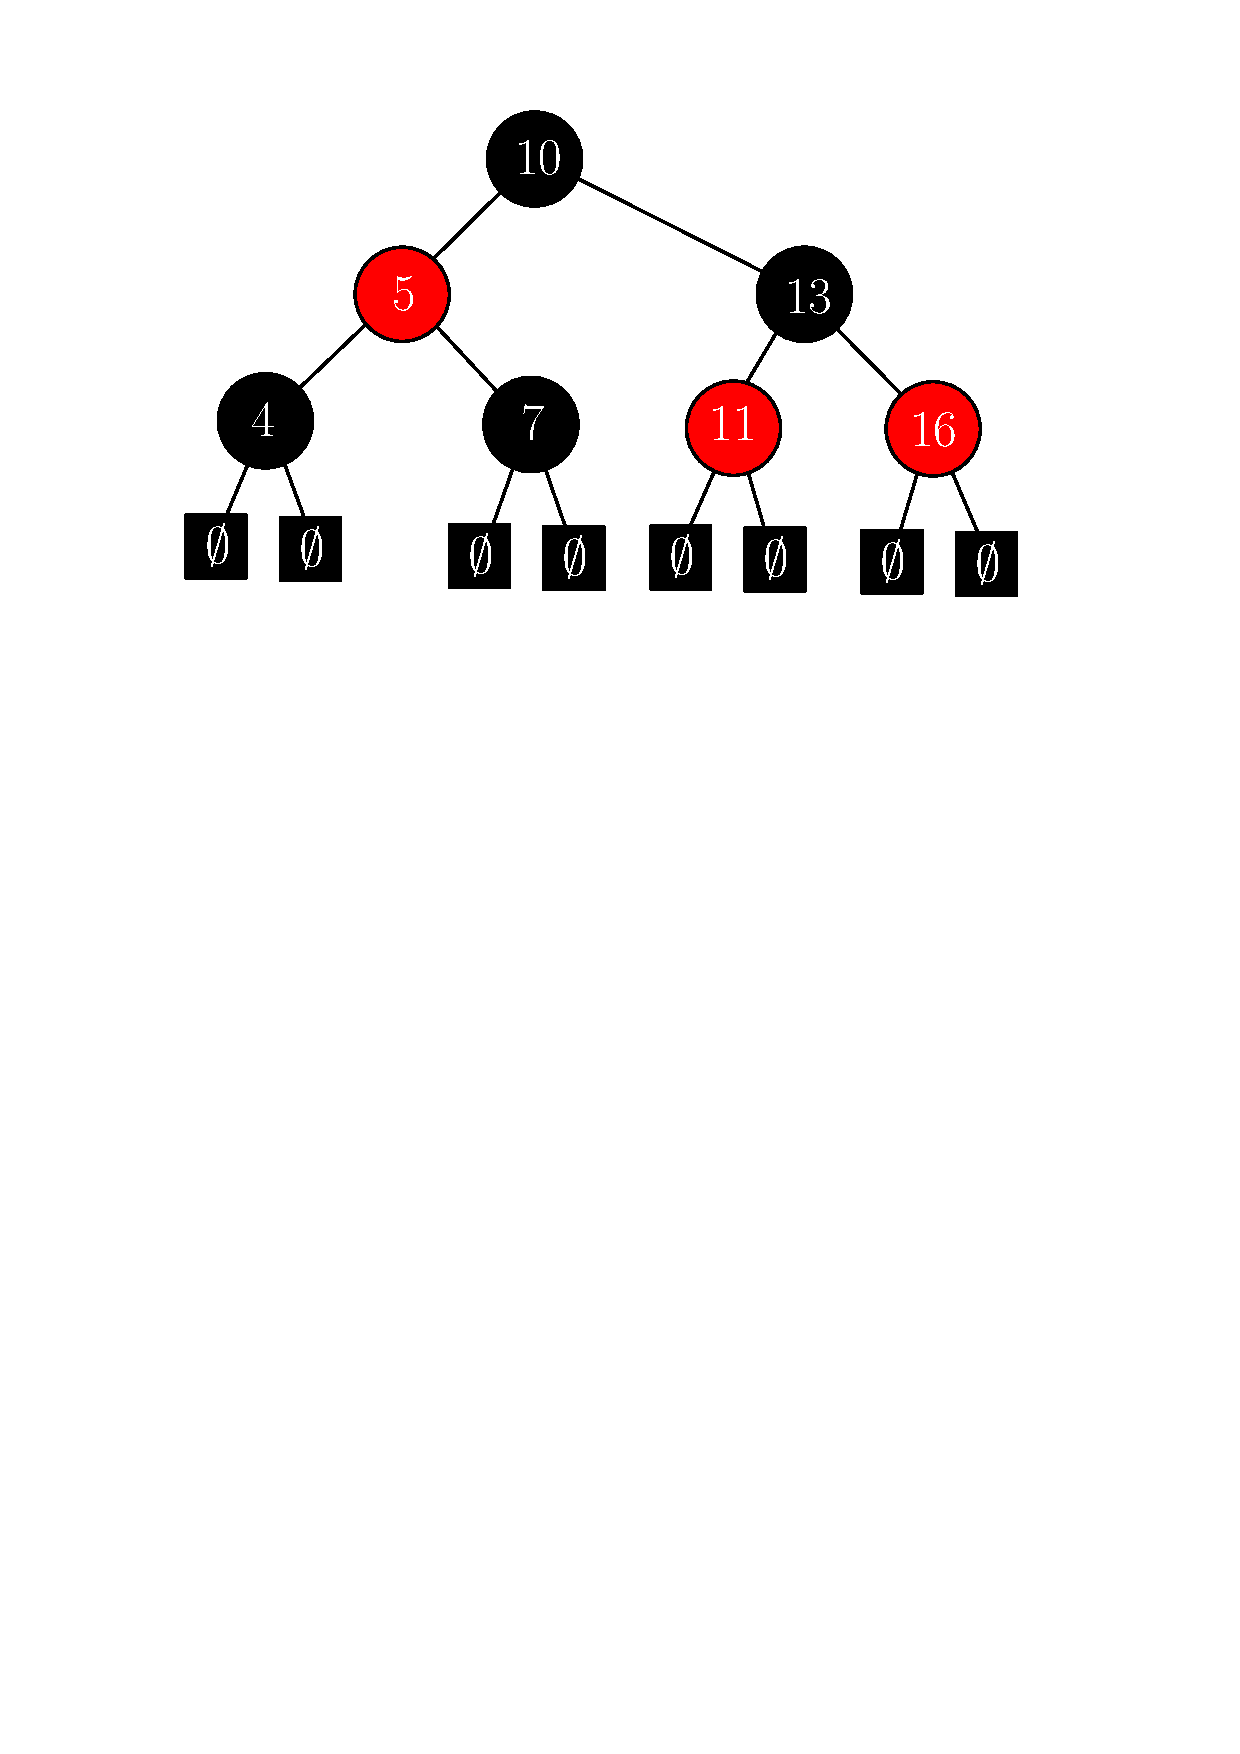
\includegraphics[height=50mm]{./images/redblack1.pdf}
	\caption{Ein rot-schwarz-Baum. Die rechteckigen Knoten repr\"asentieren die $\emptyset$-Zeiger f\"ur {\bf RB3}.}
\end{figure}

\begin{lemma}\label{lem_rb}
	Ein rot-schwarz-Baum mit $n$ Knoten hat H\"ohe $O(\log n)$.
\end{lemma}
\begin{proof}
	Dies folgt unmittelbar aus {\bf RB4} und {\bf RB5}.
\end{proof}

\subsection{Rotationen}\label{sec_rb_rot}
Rotationen sind eine Hilfsoperation, die wir f\"ur die {\tt Insert} und {\tt Delete}-Operationen auf rot-schwarz-B\"aumen ben\"otigen.
Rotationen erhalten {\em nicht unbedingt} die Eigenschaften {\bf RB1}--{\bf RB5}.
Abbildung~\ref{fig_rotate} stellt die Operationen dar.
Rotationen k\"onnen in Zeit $O(1)$ ausgef\"uhrt werden, weil nur einige Zeiger auf Kind/Elternknoten ``umgeh\"angt'' werden m\"ussen.

\begin{figure}
	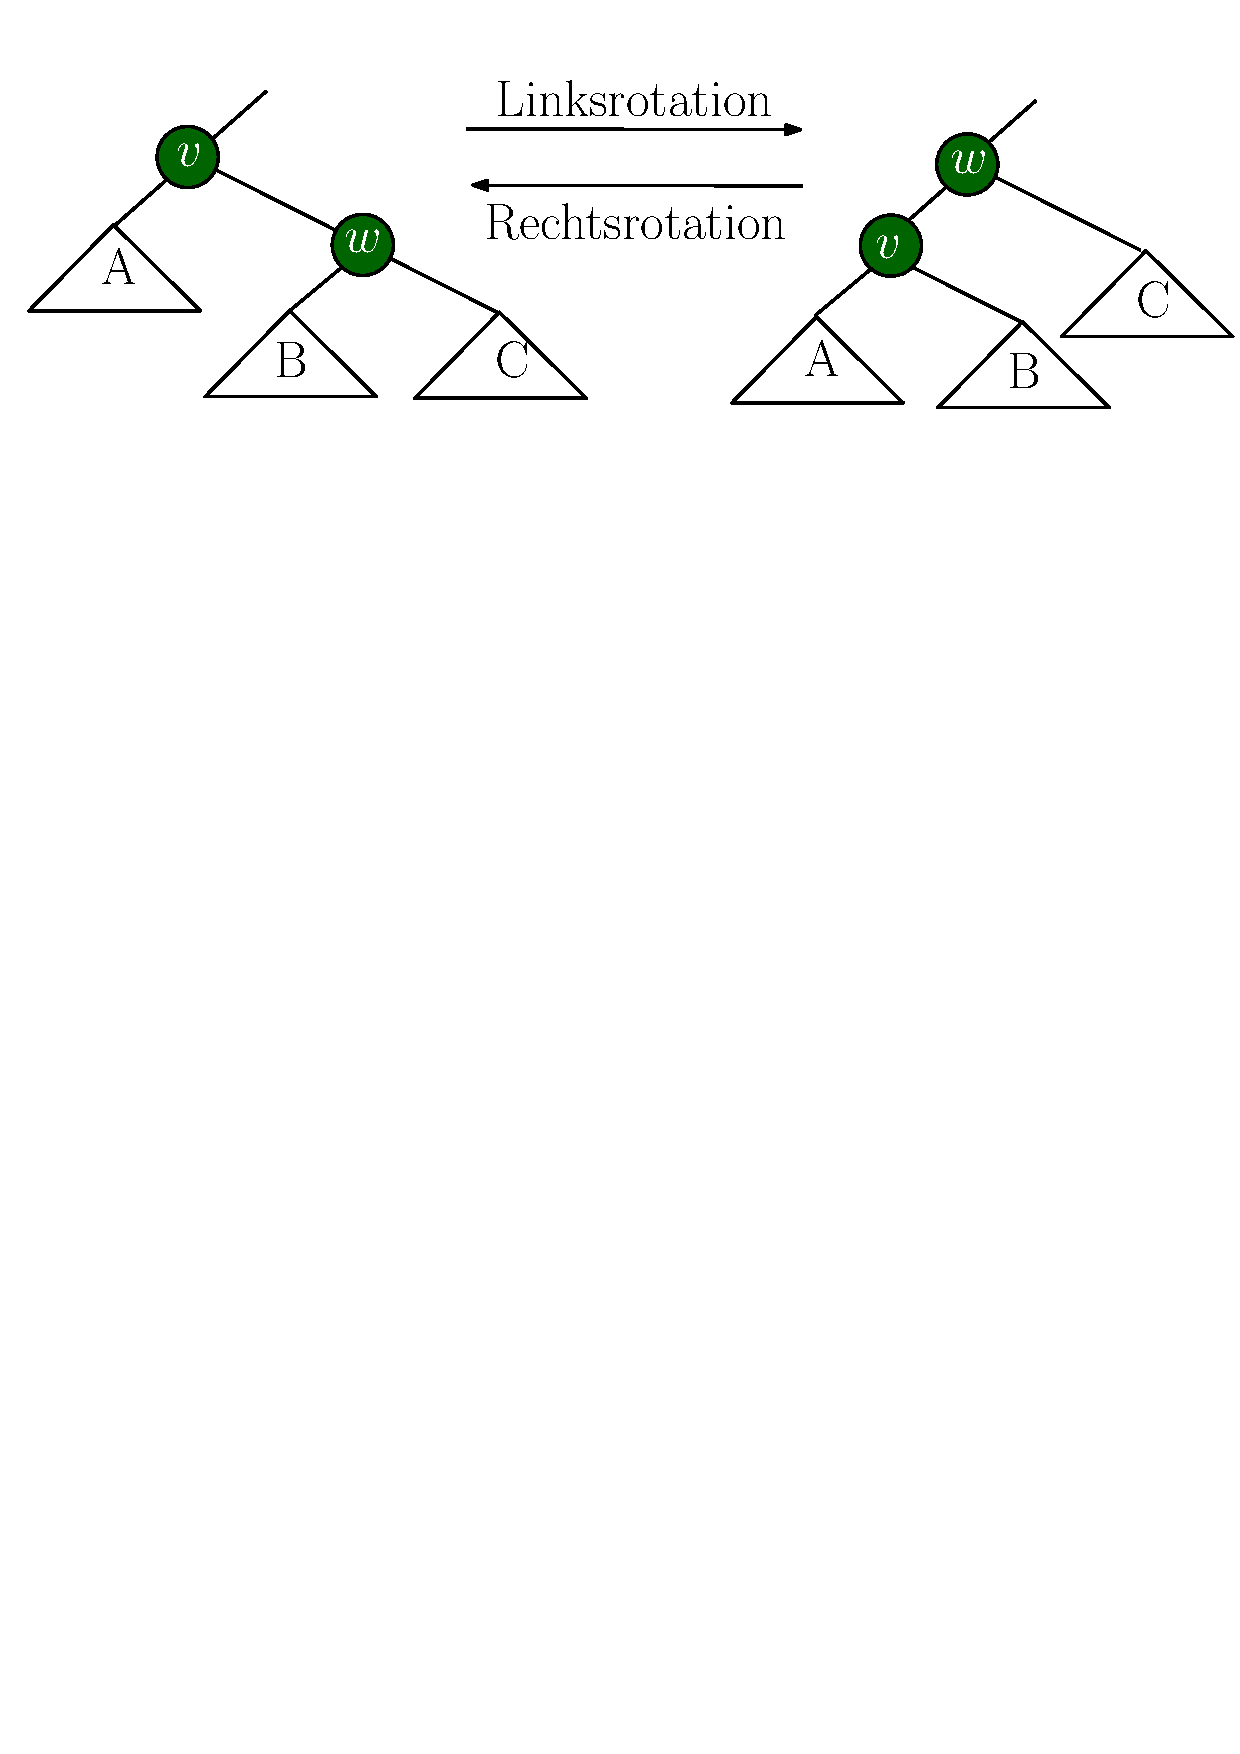
\includegraphics[height=30mm]{./images/rotate1.pdf}
	\caption{Eine Linksrotation um $v$ und eine Rechtsrotation um $w$}\label{fig_rotate}
\end{figure}

\subsection{Einf\"ugen neuer Knoten}\label{sec_rb_insert}

Zun\"achst wird der neue Knoten genau wie in einem gew\"ohnlichen bin\"aren Suchbaum eingef\"ugt (s.\ Abschnitt~\ref{sec_binary_insert}).
Der neu eingef\"ugte Knoten wird {\em rot} gef\"arbt.
Dadurch k\"onnen Eigenschaften {\bf RB2} oder {\bf RB4} verletzt werden.
Daher ist anschlie\ss end die folgende ``Aufr\"aumaktion'' notwendig.

\begin{algorithm}\upshape {\tt InsertCleanup}. {\em Eingabe:} $(T,r)$ und der eingef\"ugte Knoten $z$.
	\begin{enumerate}
		\item solange $\pi(z)$ rot ist
		\item $\quad$wenn $\pi(z)$ ein linkes Kind ist
		\item $\qquad$sei $y$ das rechte Kind von $\pi(\pi(z))$
		\item $\qquad$falls $y$ rot ist, f\"arbe $y$ und $\pi(z)$ schwarz und $\pi(\pi(z))$ rot; setze $z=\pi(\pi(z))$
		\item $\qquad$sonst:
		\item $\quad\qquad$falls $z$ ein rechtes Kind ist, setze $z=\pi(z)$ und f\"uhre dann eine Linksrotation um $z$ aus
		\item $\quad\qquad$f\"arbe $\pi(z)$ schwarz und $\pi(\pi(z))$ rot
		\item $\quad\qquad$f\"uhre eine Rechtsrotation um $\pi(\pi(z))$ aus
		\item $\quad$sonst (wenn also $\pi(z)$ ein rechtes Kind ist) \hfill // symmetrisch, mit links/rechts vertauscht
		\item $\qquad$sei $y$ das linke Kind von $\pi(\pi(z))$
		\item $\qquad$falls $y$ rot ist, f\"arbe $y$ und $\pi(z)$ schwarz und $\pi(\pi(z))$ rot; setze $z=\pi(\pi(z))$
		\item $\qquad$sonst:
		\item $\quad\qquad$falls $z$ ein linkes Kind ist, setze $z=\pi(z)$ und f\"uhre dann eine Rechtsrotation um $z$ aus
		\item $\quad\qquad$f\"arbe $\pi(z)$ schwarz und $\pi(\pi(z))$ rot
		\item $\quad\qquad$f\"uhre eine Linksrotation um $\pi(\pi(z))$ aus
		\item f\"arbe die Wurzel des Baums schwarz
	\end{enumerate}
\end{algorithm}

Die Operationen hat Laufzeit $O(\log n)$ und stellt sicher, da\ss\ anschlie\ss end die Bedingungen {\bf RB1--RB5} erf\"ullt sind.
Auf den Folien zur Vorlesung sind einige Beispiele zu finden.

\subsection{Entfernen von Knoten}\label{sec_rb_delete}

Ebenso wie beim Einf\"ugen wird auch beim Entfernen zun\"achst wie im Fall gew\"ohnlicher bin\"arer Suchb\"aume verfahren.
Allerdings ist wiederum eine Aufr\"aumaktion notwendig. 
Die folgende Operationen wird aufgerufen f\"ur den Knoten $x$ aus Algorithmus~\ref{alg_del}.

\begin{algorithm}\upshape {\tt DeleteCleanup}. {\em Eingabe:} $(T,r)$ und der Knoten $x$.
	\begin{enumerate}
		\item solange $x$ nicht die Wurzel von $T$ ist und $x$ schwarz ist
		\item $\quad$falls $x$ ein linkes Kind ist
		\item $\qquad$setze $w=\rho(\pi(x))$ \hfill//Geschwisterkonten von $x$
		\item $\qquad$falls $w$ rot ist
		\item $\quad\qquad$f\"arbe $w$ schwarz und $\pi(x)$ rot
		\item $\quad\qquad$f\"uhre eine Linksrotation um $\pi(x)$ aus und setze dann $w=\rho(\pi(x))$
		\item $\qquad$falls $\lambda(w)$ und $\rho(w)$ beide schwarz sind, f\"arbe $w$ rot und setze $x=\pi(x)$
		\item $\qquad$sonst
		\item $\quad\qquad$falls $\rho(w)$ schwarz ist
		\item $\qquad\qquad$f\"arbe $\lambda(w)$ schwarz und $w$ rot 
		\item $\qquad\qquad$f\"uhre eine Rechtsrotation um $w$ aus
		\item $\qquad\qquad$setze $w=\rho(\pi(x))$
		\item $\quad\qquad$f\"arbe $w$ mit derselben Farbe wie $\pi(x)$
		\item $\quad\qquad$f\"arbe $\pi(x)$ und $\rho(w)$ schwarz
		\item $\quad\qquad$f\"uhre eine Linksrotation um $\pi(x)$ aus
		\item $\quad\qquad$setze $x$ auf die Wurzel von $T$ (und breche somit die ``solange''-Schleife ab)
		\item $\quad$sonst (falls $x$ ein rechtes) Kind ist
		\item $\qquad${\em wie Schritte (2)--(16) mit ``links'' und ``rechts'' vertauscht}
		\item f\"arbe $x$ schwarz
	\end{enumerate}
\end{algorithm}

Auch die {\tt DeleteCleanup}-Operation hat Laufzeit $O(\log n)$.
Sie stellt die Bedingungen {\bf RB1--RB5} wieder her.
Auf den Folien zur Vorlesung sind einige Beispiele zu finden.

\section{Binomial heaps}\label{sec_binomial}

\noindent
Binomial heaps sind eine alternative Umsetzung von priority queues.
Mit ihnen l\"a\ss t sich beispielsweise der Dijkstra-Algorithmus recht gut implementieren.
Der Flaschenhals dabei ist ja jeweils die Berechnung des Knotens mit dem minimalen Abstand.
Der binomial heap beschleunigt diese Operation.

Binomial heaps unterst\"utzen die folgenden Operationen:
\begin{description}
	\item[einf\"ugen:] neues Element mit gegebenen Gewicht hinzuf\"ugen
	\item[Minimum:] auffinden des Elements mit minimalen Gewicht
	\item[Minimum entnehmen:] auffinden und entfernen
	\item[Vereinigung:] zwei Heaps zu einem vereinigen
	\item[verringern:] das Gewicht eines Elements verringern
	\item[l\"oschen:] ein Element aus der Datenstruktur entfernen
\end{description}
Wir werden sehen, da\ss\ alle diese Operationen Laufzeit $O(\log n)$ haben.

Bemerkenswert ist, da\ss\ auch die Vereinigung zweier binomial heaps in Zeit $O(\log n)$ m\"oglich ist (wobei $n$ die Zahl der Elemente der Vereinigung ist)!
Allerdings werden dabei die beiden zu vereinigenden Heaps ``zerst\"ort''.

\subsection{Binomialb\"aume}\label{sec_binomial_trees}
Da binomial heaps aus Binomialb\"aumen zusammengesetzt sind, befassen wir uns zun\"achst mit letzteren.

\begin{definition}\label{def_binomial_tree}
	Ein Binomialbaum ist ein geordneter, gewurzelter Baum, d.h.\ ein Knoten ist als Wurzel ausgezeichnet.
	Ferner sind die Kinder jedes Knotens geordnet.
	Zu jeder \alert{Ordnung} $k\geq0$ gibt es genau einen Binomialbaum (bis auf Isomorphie):
	\begin{itemize}
		\item der Binomialbaum der Ordnung $0$ besteht nur aus einem Knoten.
		\item der Baum der Ordnung $k\geq1$ entsteht aus zwei B\"aumen der Ordnung $k-1$, wobei der erste Baum links an die Wurzel des zweiten Baums angeh\"angt wird.
	\end{itemize}
\end{definition}

\noindent
In einem Binomialbaum der Ordnung $k$ h\"angt an der Wurzel also jeweils ein Baum der Ordnung $0,1,\ldots,k-1$.

\begin{lemma}\label{lem_binomial_tree}
	Der Binomialbaum $B_k$ der Ordnung $k\geq0$ hat folgende Eigenschaften
	\begin{itemize}
		\item die Zahl der Knoten ist $2^k$
		\item die H\"ohe des Baums ist $k$
		\item es gibt genau $\binom kh$ Knoten auf Tiefe $h$ f\"ur $h=0,\ldots,k$
		\item die Wurzel hat Grad $k=\Delta(B_k)$
	\end{itemize}
	\itshape Die Tiefe eines Knotens ist definiert als der Abstand von der Wurzel.
\end{lemma}
\begin{proof}
	Wir f\"uhren Induktion nach $k$.
	Item im Fall $k=0$ gelten die gew\"unschten Eigenschaften.
	F\"ur $k>0$ folgen die Behauptungen zu Knotenzahl, H\"ohe und Grad der Wurzel unmittelbar aus der Induktionsvoraussetzung
	Die Zahl der Knoten auf Tiefe $0\leq h\leq k$ berechnet sich nach Induktion zu
	$$\binom kh+\binom k{h-1}=\binom{k+1}h$$
	Es gibt genau einen Knoten auf Tiefe $k+1$
\end{proof}

\subsection{Konstruktion von binomial heaps}\label{sec_binomial_heaps}

Ein binomial heap besteht aus binomial trees verschiedener Ordnungen.

\begin{definition}\label{def_binomial_heap}
	Ein binomial heap ist eine verkettete Liste von Binomialb\"aumen.
	Genauer sei $n\ge1$ eine ganze Zahl mit Bin\"ardarstellung 
	\begin{align*}
		n&=\sum_{j=0}^\ell b_j2^j&&\mbox{ mit }&&b_j\in\{0,1\},\ b_\ell=1.
	\end{align*}
	Dann enth\"alt der binomial heap der Ordnung $n$ genau $b_j$ Binomialb\"aume der Ordnung $j$ f\"ur $j=0,\ldots,\ell$
	Diese Binomialb\"aume bilde eine der Ordnung nach aufsteigend geordnete verkettete Liste.
	Jeder einzelne Binomialbaum besteht aus einem Zeiger auf die Wurzel.
	Jeder Knoten ausser der Wurzel verf\"ugt \"uber einen Zeiger auf seinen Elternknoten.
	Ferner besitzt jeder Knoten einen Zeiger auf den n\"achsten Geschwisterknoten.
\end{definition}

Der binomial heap besteht also aus $O(\log n)$ B\"aumen mit maximaler Tiefe $O(\log n)$.
Innerhalb jedes Baumes ist das Gewicht des Elternknotens immer kleiner oder gleich dem Gewicht jedes Kindknotens.
Insbesondere hat der Wurzelknoten das geringste Gewicht.
Allerdings sind die Gewichte der Wurzelknoten im binomial heap sind nicht notwendigerweise geordnet.

\subsection{Operationen auf binomial heaps}\label{sec_binomial_heaps_ops}
Die oben genannten Operationen lassen sich nun leicht implementieren.
Die gr\"o\ss te Umsicht ist bei der Vereinigungsoperation geboten, die als Helfer bei den anderen Operationen fungiert.

\subsubsection{Minimum finden}
Das Element minimalen Gewichts finden wir, indem wir einfach die Wurzelknoten der B\"aume des binomial heap durchsuchen.
Das funktioniert, weil in jedem einzelen binomial tree die Wurzel das Element minimalen Gewichts ist.
Der Zeitbedarf bel\"auft sich auf $O(\log n)$.

\subsubsection{Vereinigung}

Um zwei binomial heaps $B_1,B_2$ zu vereinigen, f\"ugen wir zun\"achst die Listen der Binomialb\"aume zusammen.
Beim Zusammenf\"ugen wird die Ordnung beibehalten.
Es treten also zu jeder Ordnung $j$ h\"ochsts {\em zwei} B\"aume der Ordnung $j$ auf; beim Vereinigungsprozess kann zeitweilig ein dritter Baum einer gegebenen Ordnung entstehen.

Um die binomial heap-Struktur wiederherzustellen,  gehen wir die vereinige Liste der B\"aume durch.
Wenn von einer Ordnung genau zwei B\"aume vorkommen, vereinigen wir sie.
Wenn von einer Ordnung drei B\"aume vorkommen, behalten wir den ersten bei und vereinigen die beiden anderen.
Dabei stellen wir sicher, da\ss\ die Wurzel das Element geringsten Gewichtes bleibt.
Die Laufzeit f\"ur den Vereinigungsprozess liegt somit bei $O(\log n)$.

\subsubsection{Einf\"ugen}
Zum Einf\"ugen eines neuen Elementes in eine binomial heap $H$ legen wir einen binomial heap $H'$ der Ordnung $0$ an, der \emph{nur} das neue Element enth\"alt.
Dann bilden wir die Vereinigung von $H$ und $H'$.
Die Laufzeit betr\"agt $O(\log n)$.

\subsubsection{Minimum entnehmen}

Finde zun\"achst das Element $x$ minimalen Gewichts in $H$.
Nach Konstruktion ist dieses Element ist Wurzel eines Binomialbaums $T$.
Bilde nun einen neuen binomial heap $H'$, dessen Elemente die Kinder von $T$ (in umgekehrter Reihenfolge) sind und vereinige $H'$ mit dem binomial heap $H''=H-T$ .
Die Laufzeit betr\"agt $O(\log n)$.

\subsubsection{Gewicht verringern}

Um das Gewicht eines Elements $x$ zu verringern, m\"ussen nur die Elemente des Baums, dem $x$ angeh\"ort, neu angeordnet werden.
Genauer lassen wir $x$ in Richtung Wurzel aufsteigen, bis alle Kinder von $x$ mindestens das Gewicht von $x$ haben.
Die Laufzeit betr\"agt $O(\log n)$, weil die Tiefe des Baums $O(\log n)$ ist.

\subsubsection{L\"oschen}
Wir setzen das Gewicht des zu l\"oschenden Elements auf $-\infty$ und entfernen anschlie\ss end das Minimum.
Damit kommen wir auf Laufzeit $O(\log n)$.

\section{AVL-B\"aume}\label{sec_avl}

\noindent
Bei AVL-B\"aumen, benannt nach ihren Erfindern Adelson, Velsky und Landis, handelt es sich um eine weitere Variante selbstbalancierender bin\"arer Suchb\"aume.
Sie stellen somit eine Alternative zu rot-schwarz-B\"aumen dar.
Allerdings sind AVL-B\"aume strikter balanciert.

\begin{definition}\label{def_avl}
	Ein AVL-Baum ist ein gewurzelter bin\"arer Suchbaum, in dem sich f\"ur jeden Knoten $v$ die H\"ohe des linken und des rechten Teilbaums um h\"ochstens eins unterscheidet.
\end{definition}

Alle Operationen f\"ur bin\"are Suchb\"aume haben auch auf AVL-B\"aumen Laufzeit $O(\log n)$.
Wie im Fall von rot-schwarz-B\"aumen m\"ussen wir uns lediglich \"uber die Operationen zum Einf\"ugen und Entfernen von Elementen Gedanken machen, da die folgende Aussage die H\"ohe von AVL-B\"aumen beschr\"ankt.

\begin{proposition}\label{prop_avl}
	Ein AVL-Baum mit $n$ Elementen hat H\"ohe $O(\log n)$.
\end{proposition}
\begin{proof}
	Dies folgt mit einer einfachen Induktion aus der Definition.
\end{proof}

Wie im Fall der rot-schwarz-B\"aume verwenden wir Rotationen, um den Baum nach dem Einf\"ugen oder L\"oschen eines Elements zu rebalancieren.
Zu diesem Zweck statten wir jeden Knoten $v$ des Baums mit einem zus\"atzlichen Eintrag $\beta(v)$ aus, n\"amlich
\begin{align*}
	\beta(v)&=\mbox{H\"ohe des rechten Teilbaums von $v$}-\mbox{H\"ohe des linken Teilbaums von $v$}.
\end{align*}
In einem AVL-Baum gilt offenbar $\beta(v)\in\{-1,0,1\}$.
Im Zuge des Einf\"ugens und Entfernens werden wir diese Eintr\"age entsprechend aktualisieren.

\subsection{Einf\"ugen}\label{sec_avl_insert}
Wir f\"ugen zun\"achst einen neuen Knoten $z$ wie in einen gew\"ohnlichen bin\"aren Suchbaum ein (Abschnitt~\ref{sec_binary_insert}).
Dadurch kann nat\"urlich die AVL-Eigenschaft zerst\"ort werden.
Um diese wiederherzustellen, f\"uhren wir folgende Operation aus.
Dabei bezieht sich $\beta$ stets auf den Balancewert {\em vor} dem Einf\"ugen des neuen Knotens $z$.

\begin{algorithm}\upshape {\tt InsertRebalance}. {\em Eingabe:} $(T,r)$ und der Knoten $z$.
	\begin{enumerate}
		\item falls $z$ die Wurzel ist, halte.
		\item sei $p$ der Elternknoten von $z$.
		\item falls $z$ das rechte Kind von $p$ ist
		\item $\quad$falls $\beta(p)>0$
		\item $\qquad$falls $\beta(z)<0$
		\item $\quad\qquad$f\"uhre eine Rechtsrotation um $z$ und anschlie\ss end eine Linksrotation um $p$ aus
		\item $\qquad$sonst f\"uhre eine Linksrotation um $p$ aus
		\item $\quad$sonst
		\item $\qquad$falls $\beta(p)<0$, setze $\beta(p)=0$ und halte
		\item $\qquad$sonst setze $\beta(p)=1$ und rufe rekursiv {\tt InsertRebalance}$(T,r,p)$ auf
		\item sonst verfahre analog wie oben mit links/rechts vertauscht
	\end{enumerate}
\end{algorithm}

Bei den Rotationsoperationen m\"ussen jeweils die $\beta$-Eintr\"age der Knoten aktualisiert werden.
Abgesehen davon sind die Rotationen identisch zu denen, die wir bei den rot-schwarz-B\"aumen kennengelernt haben.

\subsection{Entfernen}\label{sec_avl_delete}
Zum Entfernen einens Knotens verfahren wir zun\"achst wiederum wie im Fall gew\"ohnlicher bin\"arer Suchb\"aume.
Dabei verringert sich die H\"ohe eines Kindes $z$ um eins.
Uns von diesem Knoten aus auf die Wurzel zubewegend, f\"uhren wir wiederum Rotationen aus, um die AVL-Eigenschaft wiederherzustellen.

\begin{algorithm}\upshape {\tt DeleteRebalance}. {\em Eingabe:} $(T,r)$ und der Knoten $z$.
	\begin{enumerate}
		\item falls $z$ die Wurzel ist, halte.
		\item sei $p$ der Elternknoten von $z$ und $y$ der Schwesterkonten von $z$ (bzw.\ $y=\emptyset$)
		\item falls $z$ das linke Kind von $p$ ist
		\item $\quad$falls $\beta(p)>0$
		\item $\qquad$falls $\beta(y)<0$
		\item $\quad\qquad$f\"uhre eine Rechtsrotation um $y$ und anschlie\ss end eine Linksrotation um $p$ aus
		\item $\qquad$sonst f\"uhre eine Linksrotation um $p$ aus
		\item $\quad$sonst
		\item $\qquad$falls $\beta(p)=0$, setze $\beta(p)=1$ und halte
		\item $\qquad$sonst setze $\beta(p)=0$ und rufe rekursiv {\tt DeleteRebalance}$(T,r,p)$ auf
		\item sonst verfahre analog wie oben mit links/rechts vertauscht
	\end{enumerate}
\end{algorithm}

Wie beim Einf\"ugen sind bei den Rotationsoperationen jeweils die $\beta$-Eintr\"age zu aktualisieren.


\begin{thebibliography}{99}
	\bibitem{Cormen}T.~Cormen, C.~Leiserson, R.~Rivest, C.~Stein: Introduction to algorithms. MIT Press.
	\bibitem{Diestel}R.~Diestel: Graphentheorie. Springer.
	\bibitem{Knuth}D.~Knuth: The art of computer programming. Addison Wesley.
	\bibitem{Lang}S.~Lang: Undergraduate analysis. Springer.
	\bibitem{Papadimitriou}C.~Papadimitriou: Computational complexity. Addison Wesley.
\end{thebibliography}

\end{document}
